\documentclass[conference]{IEEEtran}
\IEEEoverridecommandlockouts

% Core packages
\usepackage{cite}
\usepackage[T1]{fontenc}
\usepackage{hyperref}

% Math packages
\usepackage{amsmath,amssymb,amsfonts}
\usepackage{array,booktabs}

% Graphics and layout
\usepackage{graphicx}
\usepackage{subcaption}
\usepackage{float}
\usepackage{multirow}
\usepackage{multicol}
\usepackage{balance}

% Algorithm and code
\usepackage{algorithm}
\usepackage{algpseudocode} 
\usepackage{algorithmicx}
\usepackage{listings}

% Text and formatting
\usepackage{textcomp}
\usepackage{url}
\usepackage{enumitem}
\usepackage{caption} 
\usepackage{tcolorbox}
\usepackage{empheq}
\usepackage{varwidth}
\usepackage{balance}
\usepackage{todonotes}
\usepackage{flushend} 

\usepackage[ngerman,main=english]{babel}
 
% TikZ for diagrams
\usepackage{tikz}
\usetikzlibrary{arrows.meta,shapes,positioning}
\usetikzlibrary{calc,angles,quotes}

% --- Macro for drawing a 2D spherocylinder ---
% #1 = center coordinate
% #2 = rotation angle
% #3 = half-length
% #4 = radius
\newcommand{\drawSpherocyl}[4]{
    \begin{scope}[shift={(#1)},rotate=#2]
        \draw[line width=1pt,rounded corners=6pt] (-#3 + #4,#4) -- (#3 - #4,#4);
        \draw[line width=1pt,rounded corners=6pt] (-#3 + #4,-#4) -- (#3 - #4,-#4);
        \draw[line width=1pt,rounded corners=6pt] (#3 - #4,-#4) arc[start angle=-90,end angle=90,radius=#4];
        \draw[line width=1pt,rounded corners=6pt] (-#3 + #4,#4) arc[start angle=90,end angle=270,radius=#4];
        \fill [black] (#1) circle (2pt);
    \end{scope}
}



\hypersetup{hidelinks}
\DeclareMathAlphabet\mathbfcal{OMS}{cmsy}{b}{n}

% Macro for growth comparison row
\newcolumntype{M}[1]{>{\centering\arraybackslash}m{#1}}

\newcommand{\growthcomparisonrow}[6]{%
    #1 &
        \includegraphics[width=\linewidth]{figures/growth/#1_#2/#1_#2.#3.jpeg}
    &
        \includegraphics[width=\linewidth]{figures/growth/#1_#2/#1_#2.#4.jpeg}
    &
        \includegraphics[width=\linewidth]{figures/growth/#1_#2/#1_#2.#5.jpeg}
    &
        \includegraphics[width=\linewidth]{figures/growth/#1_#2/#1_#2.#6.jpeg}
    \\
}

\newcommand{\orientationcomparisonrow}[2]{%
    #1 &
        \includegraphics[width=\linewidth]{figures/orientation_comparisons/zoomed_images/hard_e#2_orient.jpeg}
    &   
        \includegraphics[width=\linewidth]{figures/orientation_comparisons/zoomed_images/soft_e#2_orient.jpeg}
    \\
}
 
\newcommand{\algorithmautorefname}{Algorithm}


\begin{document}

\title{Proliferating Cell Collectives: \\A Comparison of Hard and Soft Collision Models}

\author{
    \IEEEauthorblockN{Manuel Lerchner}
    \IEEEauthorblockA{
        \textit{Technical University of Munich}\\
        Munich, Germany}
}

\maketitle

\begin{abstract}
    This work investigates the computational modeling of proliferating cell collectives, comparing an established constraint-based collision model as developed by Weady et al.~\cite{Weady2024} with a simpler potential-based collision model employing a nonlinear Hertzian contact law. While both approaches are demonstrated to reproduce key emergent patterns observed in bacterial colony growth, we highlight that  ...............

\end{abstract}

\begin{IEEEkeywords}
    active matter, cell collectives, particle simulation, soft collision model, hard collision model, pattern formation, computational biology, performance comparison, agent-based modeling
\end{IEEEkeywords}

\section{Introduction}
\subsection{Biological Motivation}

The collective behaviors of biological entities, from microbial colonies to multicellular tissues, are fundamental to understanding life’s complex dynamics. These systems often exhibit emergent spatio-temporal patterns driven by local interactions and, crucially, by the growth and division of individual cells. In bacterial colonies, continuous cell proliferation at the periphery generates mechanical forces that slow growth in the densely packed center~\cite{Wittmann2023}. For species such as \textit{E. coli}, \textit{Bacillus subtilis}, and \textit{Proteus mirabilis}, as well as fungi like \textit{Setosphaeria rostrata} and \textit{Exserohilum turcicum}, this combination of expansion and central pressure produces the characteristic concentric ring patterns observed experimentally~\cite{YAMAZAKI2005136} (See \autoref{fig:exserohilum_turcicum}).

\begin{figure}[h]
    \centering
    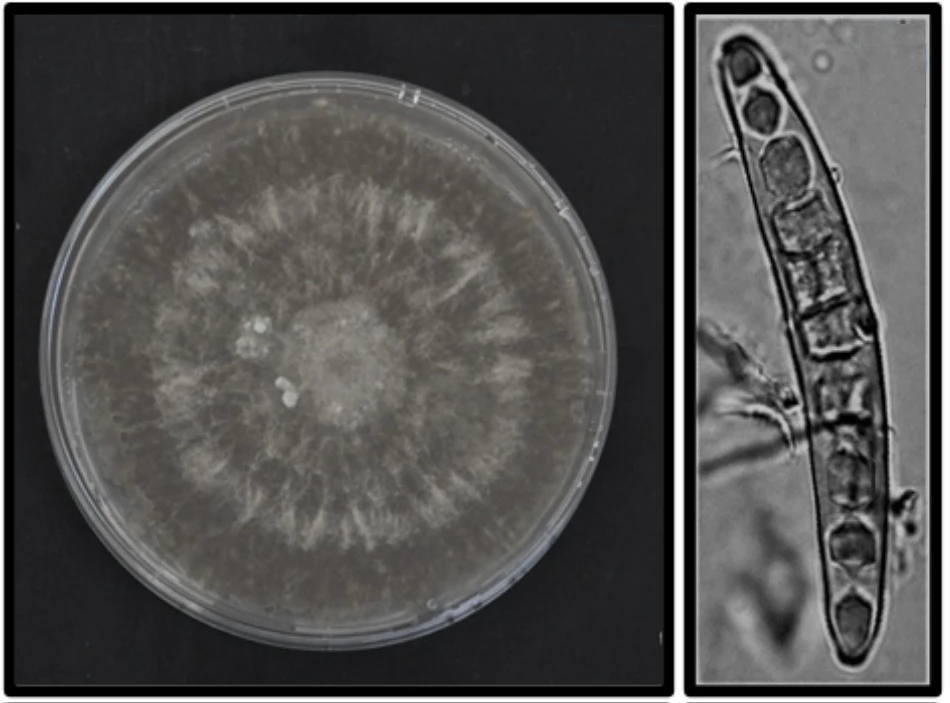
\includegraphics[width=\linewidth]{figures/real-bacteria/Exserohilum turcicum.png}
    \caption{Morphology of \textit{Exserohilum turcicum}. The left image displays a colony of \textit{Exserohilum turcicum}, while the right image shows a single cell of the same species. Source:~\cite{Bankole2023}.}
    \label{fig:exserohilum_turcicum}
\end{figure}

Understanding these emergent structures requires computational models that capture the dynamic interplay between cell growth and division, mechanical forces, and intercellular interactions. However, simulating such dense, proliferating cell collectives presents significant computational challenges, particularly in resolving cell-cell collisions efficiently and accurately.

This work is directly inspired by these observations, particularly by the work of Weady et al.~\cite{Weady2024}, who developed such a computational model to study the growth of bacterial colonies and the resulting pattern formation.



\section{Related Work}

\subsection{Collision Modeling Paradigms}


A critical computational challenge in agent-based models (ABMs) is the resolution of cell-cell collisions. Two primary paradigms exist for this purpose: potential-based (soft) and constraint-based (hard) models, each with distinct trade-offs in physical fidelity, computational cost, and numerical stability.

\begin{description}[style=nextline]
    \item[Potential-Based (Soft) Collision Models]
        These models manage interactions by employing repulsive forces, defined by potentials like Hertzian or Lennard-Jones, when agents overlap. Their primary advantage is computational tractability, as they rely on local force calculations that are highly amenable to parallelization. This has enabled large-scale simulations, such as the work by~\cite{Warren2019}, who modeled millions of cells in 3D. However, a well-known limitation is numerical stiffness, which forces the use of small integration timesteps to maintain stability. Furthermore, as noted by~\cite{Yan2019}, the finite range of repulsive forces causes particles to behave as soft and deformable, leading to an "effective" diameter smaller than the intended geometric size.

    \item[Constraint-Based (Hard) Collision Models]
        These models enforce strict non-overlapping geometric constraints, ensuring high physical fidelity by treating agents as truly impenetrable. A notable application is the work of~\cite{Rudge2012}, who simulated growing bacterial colonies using a constraint-based method. They highlighted its computational intensity, as resolving constraints often requires iterative, global solutions to large systems of equations, creating a potential bottleneck. However, modern implementations like that of~\cite{Yan2019} specifically address the drawbacks of soft models: they eliminate numerical stiffness—allowing timesteps to be increased by 10–100 times—and guarantee particles maintain their precise geometric dimensions. The trade-off is a higher computational cost per timestep due to the constraint-solving process.
\end{description}

\subsection{The Benchmarking Gap}

The reviewed literature presents two distinct computational philosophies. Soft models offer computational simplicity and have been scaled to high agent counts, but at the cost of numerical stiffness and compromised physical fidelity. Hard models, particularly modern implementations like that of~\cite{Yan2019}, offer a solution to these limitations, promising greater timesteps and rigorous geometry.

However, this presents a critical, unquantified trade-off: does the hard model's ability to take larger timesteps outweigh its inherently higher computational cost per timestep? This question is especially pertinent in simulations of proliferating cell collectives, where exponentially increasing density dramatically alters the computational load of the collision resolution algorithm.

A systematic benchmarking focusing on this computational trade-off between the models is largely absent. Existing studies~\cite{Rudge2012,Weady2024,Blanchard2015,Ghosh2015,You2018,Warren2019,Khan_2024,You_2021} typically validate their models by comparing simulation results to experimental data (e.g., microscopy images of bacterial colonies)~\cite{Rudge2012,Khan_2024, Rudge2013,Langeslay_2023, Ghosh2015}, prioritizing biological insights over a rigorous HPC analysis of runtime, scalability, and numerical stability under proliferation. Consequently, there is no clear guidance for modelers on which paradigm is more efficient for a given problem scale. This work aims to fill this gap by implementing both models within a unified ABM framework to provide a direct, quantitative comparison of their computational performance.

\section{Cell Mechanics}

The mechanical representation of cells is a critical factor in determining simulation outcomes. For many bacteria and fungal hyphae, approximating them as rigid rods is a reasonable simplification that captures their elongated morphology and the primary drivers of their collective behavior. Although real cells exhibit some degree of flexibility and deformability, the rigid rod model effectively captures the essential mechanics of cell-cell interactions and colony expansion, reproducing key emergent patterns observed experimentally~\cite{Rudge2012,Khan_2024,Rudge2013,Langeslay_2023,Ghosh2015}.

This choice of rigid rod geometry is well-supported by experimental observations and aligns with established practices in modeling microbial systems. The following collision models are applied to these rigid rod entities.

\subsection{Physical Cell Model}

We model the cell collective using a rigid rod representation, where each cell has a defined length and radius. This approach is common in models of cellular collectives~\cite{You2018, Weady2024,Weady2024SM, Blanchard2015, Warren2019, Ghosh2015} and is justified by experimental evidence, closely matching the morphology of common bacteria and fungi such as E. coli and Setosphaeria rostrata (see \autoref{fig:exserohilum_turcicum}).

Following the established literature, each bacterium is modeled as a spherocylinder with a variable length $\ell$ and a constant diameter $d$. At the bacterial scale, the Reynolds number is extremely small (Re $\ll 1$), placing the system firmly in the overdamped regime where viscous forces dominate inertial forces~\cite{datta2024lifelowreynoldsnumber,Rudge2012 }. Consequently, the dynamics are governed by the overdamped Langevin equation:

\begin{equation} \label{eq:overdamped_langevin}
    \frac{d \mathbf{x}_i}{dt} = \frac{1}{\zeta l_i} \sum_j \mathbf{F}_{ij}, \quad \frac{d \boldsymbol{\omega}_i}{dt} = \frac{12}{\zeta l_i^3} \sum_j (\mathbf{r}_{ij} \times \mathbf{F}_{ij})
\end{equation}

where $\mathbf{x}_i$ is the position of the $i$-th cell, $\boldsymbol{\omega}_i$ is its orientation, and $\mathbf{F}_{ij}$ is the force exerted on cell $i$ by cell $j$. The constant $\zeta$ is a drag coefficient representing friction with the surrounding fluid, and $\mathbf{r}_{ij}$ is the vector from the center of cell $i$ to the point of contact with cell $j$.

\autoref{fig:spherocylinder_model} illustrates the spherocylinder model and the forces and torques acting on cells during a collision.


\subsection{Cell Growth and Division}

Bacterial cells grow along their longitudinal axis according to the following model, adapted from~\cite{Weady2024SM}:

\begin{equation} \label{eq:growth}
    \dot{{\ell}} = \frac{{\ell}}{\tau} e^{\lambda \sigma}
\end{equation}

where $\tau$ is a characteristic time scale, $\sigma$ is the compressive stress along the cell's main axis, and $\lambda$ is a stress sensitivity parameter. This parameter controls the growth rate and ultimately the macroscopic pattern formation of the colony.

The stress $\sigma_i$ for a cell $i$ is computed by projecting all contact forces from neighboring cells onto the cell's longitudinal axis, defined by the unit tangent vector $\hat{\mathbf{t}}_i$:

\begin{equation} \label{eq:stress}
    \sigma_i = \sum_{j} \frac{1}{2} \left| \hat{\mathbf t}_i \cdot \mathbf F_{ij} \right|
\end{equation}

For the simulations presented here, we chose an initial cell length of $\ell = 1$ and a diameter of $d = 0.5$, following. Once a cell reaches a critical length of $\ell_{crit} = 2$, it divides into two daughter cells. To prevent artificial synchronization of division events, we introduce randomness in the daughter cells' lengths, which are randomly set between $0.98\ell_0$ and $1.02\ell_0$, following the approach in~\cite{Khan_2024}.

\subsection{Rotational Diffusion}

Moreover, we add a small random rotational perturbation to the orientation of all cells at each timestep to account for Brownian rotational diffusion. This small pertubation ensures that the cells break perfect alignment over time, which is important for realistic colony morphology.


\begin{figure}[H]
    \centering


    \begin{tikzpicture}[line cap=round,line join=round,>=Stealth]

        % --- Variables ---
        \coordinate (xi) at (0.8,-0.5);
        \coordinate (xj) at (1.4,-1.8);

        \coordinate (x) at (-3,-0.5);
        \def\R{0.5}

        \drawSpherocyl{xi}{-10}{1.4}{\R}
        \drawSpherocyl{xj}{15}{1.3}{\R}

        \coordinate (contact) at  (1.85,-1.15);

        % Collision point
        \fill[black] (contact) circle (2pt) node[above right] {};

        % Force vector
        \draw[->,thick,red] (contact) -- ++($0.9*(-0.258,0.965)$) node[pos=0.9,left] {$\mathbf{F}_{ij}$};

        % Torque lever arm
        \draw[->,thick,blue,dashed] (xi) -- (contact) node[pos=0.2,below] {$\mathbf{r}_{ij}$};

        % Force vector
        \draw[->,thick,red] (contact) -- ++($0.8*(0.258,-0.965)$) node[pos=0.6,right] {$\mathbf{F}_{ji}$};

        % Torque lever arm
        \draw[->,thick,blue,dashed] (xj) -- (contact) node[pos=0.3,left] {$\mathbf{r}_{ji}$};



        % label at xi
        \node at (xi) [left] {$\mathbf{x}_i$};
        % label at xj
        \node at (xj) [below] {$\mathbf{x}_j$};


        \drawSpherocyl{x}{0}{2}{\R};

        % Add division constriction: two daughters forming
        \coordinate (left_daughter) at ($(x)+(-1,-1.25)$);
        \coordinate (right_daughter) at ($(x)+(1, -1.25)$);

        \drawSpherocyl{left_daughter}{0}{1}{\R};
        \drawSpherocyl{right_daughter}{0}{1}{\R};


        % label at x
        \node at (x) [below] {$\mathbf{x}$};
        % label at left daughter
        \node at (left_daughter) [below] {$\mathbf{x}_\text{left}$};
        % label at right daughter
        \node at (right_daughter) [below] {$\mathbf{x}_\text{right}$};

        \draw[<->,thick,dashed] ($(x) + (-2,1)$) -- ($(x) + (2,1)$) node[midway,above] {$2\ell_0$};

        \draw[<->,thick,dashed] ($(x) + (-1.5-\R-\R,-\R)$) -- ($(x) + (-1.5-\R-\R,\R)$) node[midway,left] {$d$};

        \draw[<->,thick,dashed] ($(right_daughter) + (-2.5-\R-\R,-\R)$) -- ($(right_daughter) + (-2.5-\R-\R,\R)$) node[midway,left] {$d$};

        \draw[<->,thick,dashed] ($(left_daughter) + (-1,-1)$) -- ($(left_daughter) + (1,-1)$) node[midway,below] {$\ell_0$};

        \draw[<->,thick,dashed] ($(right_daughter) + (-1,-1)$) -- ($(right_daughter) + (1,-1)$) node[midway,below] {$\ell_0$};



        % Resulting rotation around xi
        \draw[->,thick,orange]
        ($(xi)+(0.6,0.5)$) arc[start angle=0,end angle=160,radius=0.6]
        node[midway, below] {$\boldsymbol{\omega}_i$};


        % Resulting rotation around xj
        \draw[->,thick,orange]
        ($(xj)+(0.7,-0.5)$) arc[start angle=0,end angle=-150,radius=0.6]
        node[midway, above] {$\boldsymbol{\omega}_j$};

    \end{tikzpicture}
    \caption{2D schematic of the spherocylinder cell model. Each cell is represented as a rigid rod with length $\ell$ and diameter $d$. Cells grow along their longitudinal axis and divide into two daughter cells upon reaching a critical length of $2\ell_0$. Collisions generate contact forces $\mathbf{F}_{ij}$ and $\mathbf{F}_{ji}$ (red). Torque arises from the cross product of the lever arm $\mathbf{r}_{ij}$ (dashed blue) and the contact force, leading to changes in orientation $\boldsymbol{\omega}$ (orange).}
    \label{fig:spherocylinder_model}

\end{figure}

\newpage

\section{Computational Framework}

\subsection{Colony Representation}

For our implementation, we closely follow the approach described by Weady et al.~\cite{Weady2024SM} in their supplementary material. The entire bacterial colony is represented by a single global state vector $\mathbfcal{C} = [\dots, \mathbf{x}_n^\top, \mathbf{q}_n^\top, \dots]^\top \in \mathbb{R}^{7N}$, where $N$ is the number of cells. Each cell is represented by a 7-dimensional sub-vector consisting of a position vector $\mathbf{x}_n \in \mathbb{R}^3$ and a unit quaternion $\mathbf{q}_n \in \mathbb{R}^4$ representing its orientation. The lengths of all cells are stored separately in a vector $\boldsymbol{\ell} = [\dots, \ell_n, \dots]^\top \in \mathbb{R}^{N}$.

\subsection{Colony Dynamics}

The translational and angular velocities of all particles in the colony are determined by the force-velocity relationship $\mathbfcal{U} = \mathbfcal{M} \mathbfcal{F}$. Here, $\mathbfcal{F}$ is the generalized force vector for the entire colony, containing both force and torque components for each cell. Similarly, $\mathbfcal{U}$ is the generalized velocity vector containing the resulting translational and angular velocities. These vectors are structured as follows:

\begin{itemize}
    \item
          $\mathbfcal{F} = [\dots, \mathbf{f}_n^\top, \boldsymbol{\tau}_n^\top, \dots]^\top \in \mathbb{R}^{6N}$ represents the force $\mathbf{f}_n$ and torque $\boldsymbol{\tau}_n$ for the $n$-th cell.
    \item
          $\mathbfcal{M} = \text{diag}([\dots, \frac{1}{\zeta l_n}\mathbf{I}, \frac{12}{\zeta l_n^3}\mathbf{I}, \dots]) \in \mathbb{R}^{6N \times 6N}$ is a diagonal mobility matrix, consisting of the inverses of the cell's linear and angular mobility coefficients (from Eq.~\ref{eq:overdamped_langevin}) along its diagonal. Here, $\mathbf{I}$ is the $3 \times 3$ identity matrix.
    \item
          $\mathbfcal{U} = [\dots, \mathbf{u}_n^\top, \boldsymbol{\omega}_n^\top, \dots]^\top \in \mathbb{R}^{6N}$ represents the resulting translational velocity $\mathbf{u}_n$ and angular velocity $\boldsymbol{\omega}_n$ for the $n$-th cell.
\end{itemize}


Combined with a mapping function $\mathbfcal{G}$, which converts Cartesian translational and angular velocities from $\mathbb{R}^{6N}$ to the corresponding changes in position and quaternion in $\mathbb{R}^{7N}$ (as described in~\cite{Weady2024SM,Yan2022,Tasora2008}), we can express the colony's state update for an Euler timestep $\Delta t$ as:

\begin{equation} \label{eq:colony_update}
    \mathbfcal{C}^{k+1} = \mathbfcal{C}^k + \Delta t \, \mathbfcal{G} \mathbfcal{U} = \mathbfcal{C}^k + \Delta t \, \mathbfcal{G} \mathbfcal{M} \mathbfcal{F}
\end{equation}

The mapping function $\mathbfcal{G}$ is required because the colony state is represented using quaternions, whereas the dynamics are expressed in terms of angular velocities that specify an instantaneous axis of rotation and rotation rate; $\mathbfcal{G}$ converts these into quaternion derivatives, enabling consistent integration using an Euler step~\cite{Weady2024SM, Tasora2008}.


The specific implementations of the hard and soft collision models are defined by how the generalized force vector $\mathbfcal{F}$ is computed in each case.

\newpage

\subsection{Soft Collision Model}

The soft collision model treats cell-cell interactions through a continuous, potential-based repulsion. This approach, inspired by~\cite{Warren2019} and~\cite{You2018}, generates forces that smoothly increase as cells deform against each other, preventing overlap in a physically realistic manner. We specifically implement a Hertzian contact model, which is well-suited for simulating the elastic deformation of curved, cell-like objects.

The repulsive elastic force exerted on cell $i$ by cell $j$ is calculated as:

\begin{equation} \label{eq:hertzian_contact_model}
    \mathbf{F}^{\text{elastic}}_{ij} = k_{cc} \sqrt{d_0} , \delta^{3/2} \, \hat{\mathbf{n}}
\end{equation}

where $\delta$ is the overlap distance between the two spherocylinders, $d_0$ is the cell diameter, $k_{cc}$ is an elastic constant, and $\hat{\mathbf{n}}$ is the unit normal vector at the point of contact. This nonlinear force-response is characteristic of Hertzian theory and provides a smooth onset of repulsion (see \autoref{fig:hertzian_contact_model}).

\subsubsection{Total Forces and Torques}

The total force $\mathbf{f}_n$ and torque $\boldsymbol{\tau}_n$ on the $n$-th cell are the sum of all pairwise elastic interactions with its neighbors and can be computed solely based on the elastic forces $\mathbf{F}^{\text{elastic}}_{nm}$:

\begin{equation}
    \mathbf{f}_n         = \sum_{m \neq n} \mathbf{F}^{\text{elastic}}_{nm} \qquad
    \boldsymbol{\tau}_n  = \sum_{m \neq n} \mathbf{r}_{nm} \times \mathbf{F}^{\text{elastic}}_{nm}
\end{equation}

These forces and torques are assembled into the global generalized force vector $\mathbfcal{F}$. The colony dynamics are then updated by inserting $\mathbfcal{F}$ into the force-velocity relation and applying the Euler integration step defined in \autoref{eq:colony_update}.

\subsubsection{Model Parameters}

The elastic constant $k_{cc} = \frac{Y}{\zeta}$ is a crucial parameter that determines the effective stiffness of the cells. Following~\cite{You2018}, we define it as the ratio of the cell's Young's modulus $Y$ to the fluid drag coefficient $\zeta$:

Using typical values from the literature for bacteria ($Y \approx 4$ MPa~\cite{You2018, Blanchard2015} and $\zeta \approx 200$ Pa$\cdot$h~\cite{You2018}), we set $k_{cc} = 20000$ h$^{-1}$. This value ensures that the repulsive forces are sufficiently strong to prevent significant overlap but, due to its stiffness, it also poses severe limits on the stability of the numerical integration~\cite{Yan2022}. Therefore an extremely small timestep ($\mathcal{O}(10^{-5})$ h~\cite{Khan_2024, You2018, Blanchard2015}) is required to maintain stability (See \autoref{fig:simulation_time_vs_dt}).

\begin{figure}[H]
    \centering
    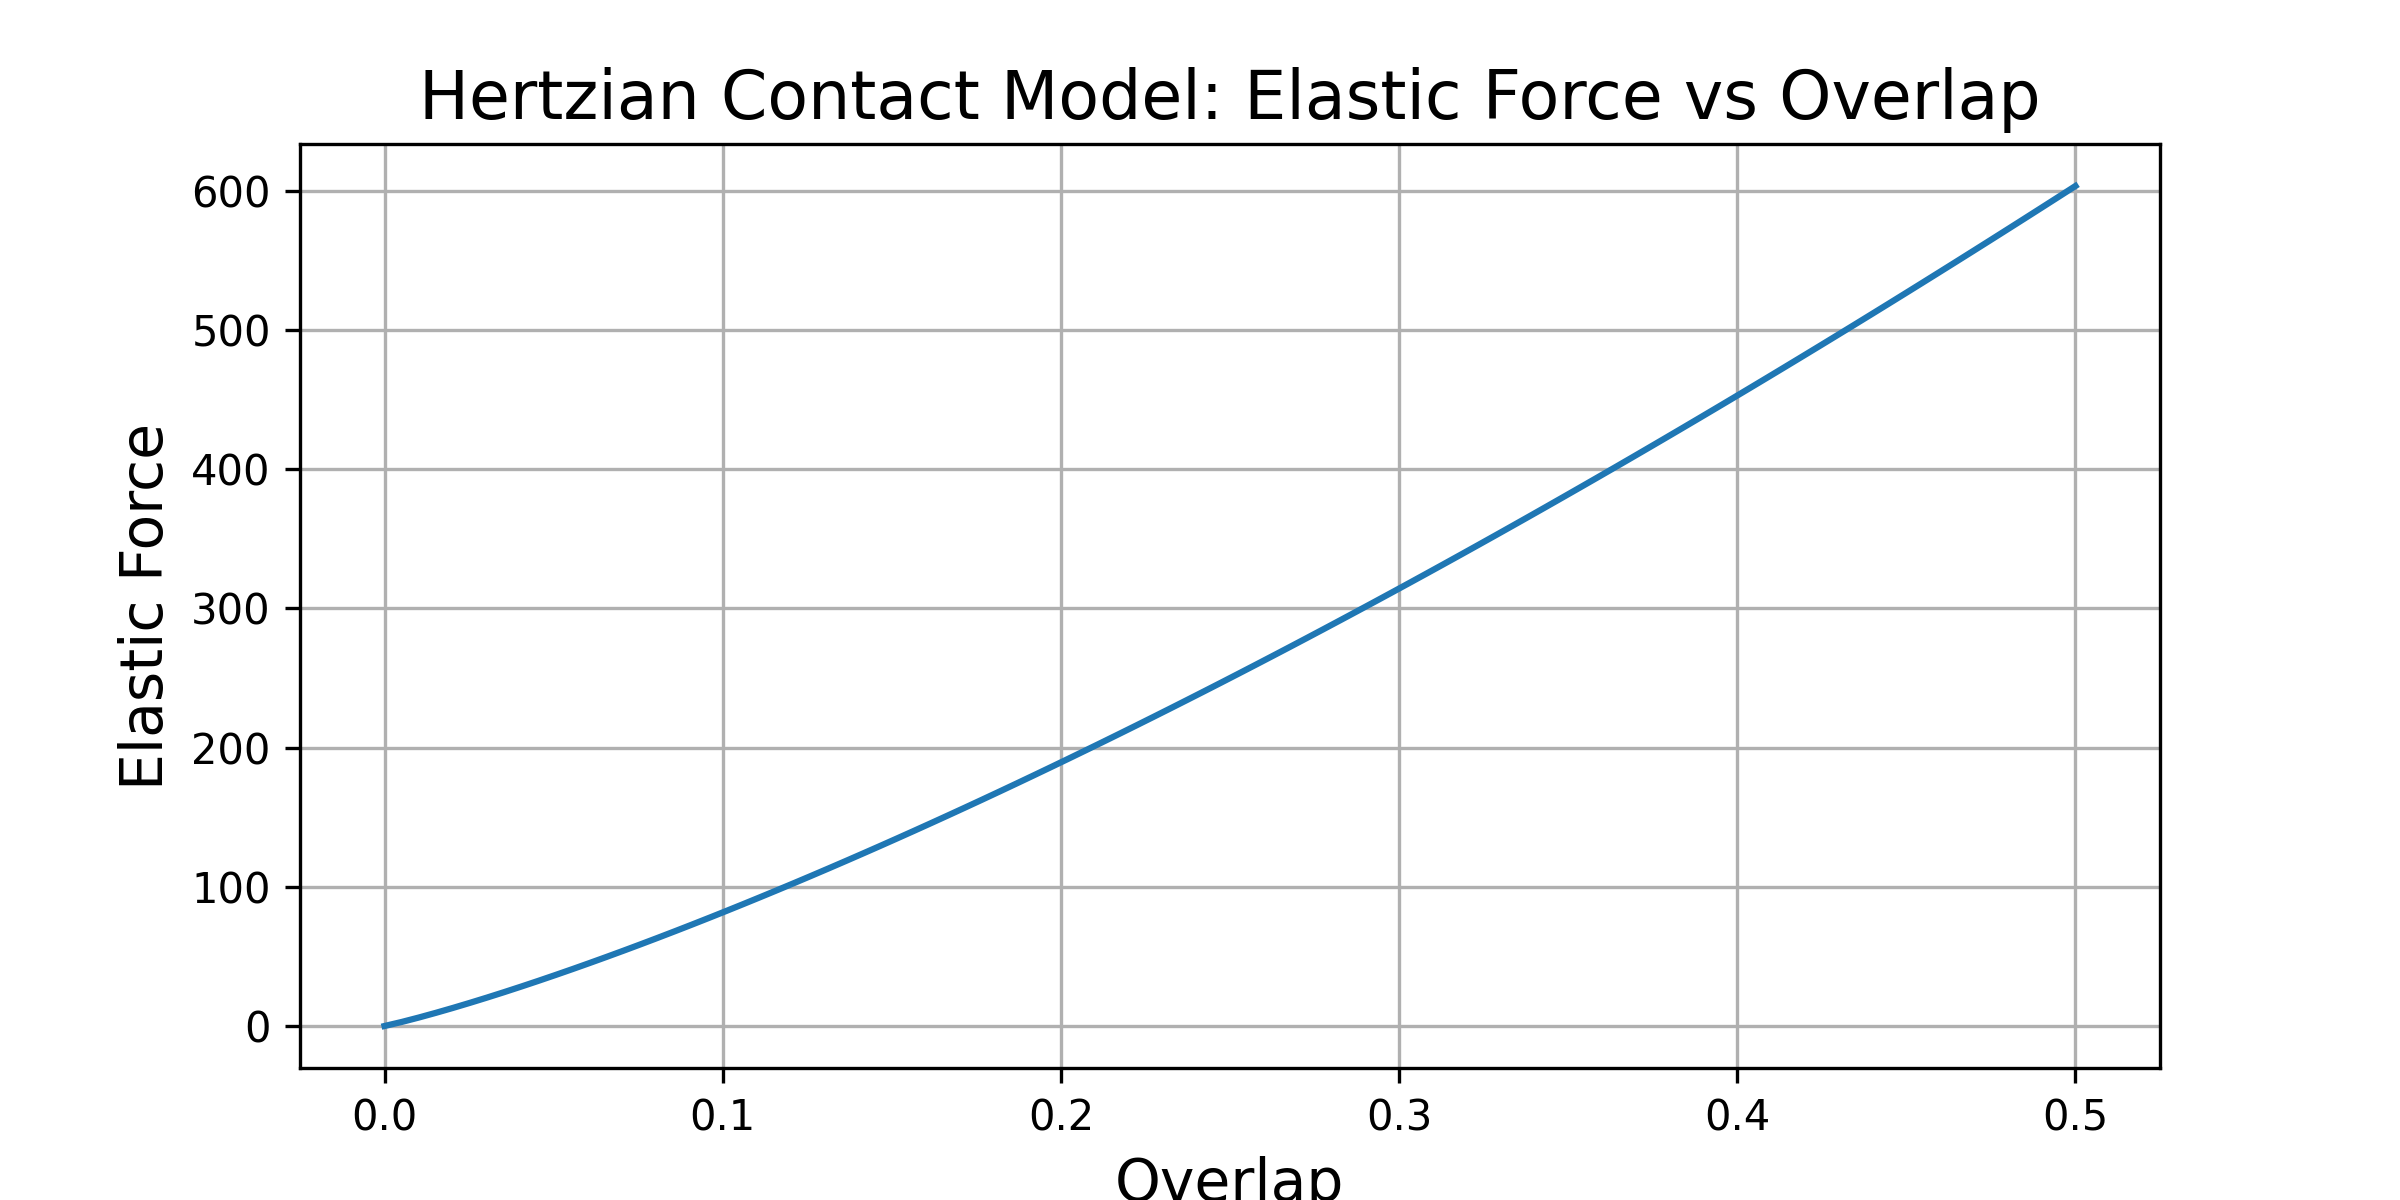
\includegraphics[width=\linewidth]{figures/hertzian_contact_model.png}
    \caption{Force response of the Hertzian contact model. The repulsive force $\mathbf{F}^{\text{elastic}}$ scales non-linearly with the overlap distance, leading to a smooth increase in repulsion.}
    \label{fig:hertzian_contact_model}
\end{figure}

\subsection{Hard Collision Model}

The hard collision model enforces strict non-overlapping constraints between cells using a constraint-based method. For each pair of nearby cells, a constraint $\alpha$ is defined based on the two closest points, $\mathbf{y}_n$ and $\mathbf{y}_m$, on their surfaces~\cite{Weady2024SM}. Contrary to the soft Hertzian model, the hard model defines the force and torque from each constraint via an yet unknown scalar Lagrange multiplier $\gamma_\alpha$. This multiplier represents the magnitude of the impulse required to prevent penetration. The force on cell $n$ due to constraint $\alpha$ is:

\begin{equation} \label{eq:constraint_force}
    \mathbf{F}^{hard}_{n\alpha} = \hat{\mathbf{n}}_\alpha \gamma_\alpha
\end{equation}

where $\hat{\mathbf{n}}_\alpha$ is the normal vector at the contact point. The corresponding torque is $\boldsymbol{\tau}_{\alpha} = (\mathbf{y}_n - \mathbf{x}_n) \times \hat{\mathbf{n}}_\alpha \gamma_\alpha$. The total generalized force vector $\mathbfcal{F}$ for the colony depends linearly on the multipliers $\boldsymbol{\gamma} = [\dots, \gamma_\alpha, \dots]^\top \in \mathbb{R}^{C}$ and can be conveniently expressed in matrix form:

\begin{equation}
    \mathbfcal{F}(\boldsymbol{\gamma}) = \mathbfcal{D} \boldsymbol{\gamma}
\end{equation}

where the sparse matrix $\mathbfcal{D} \in \mathbb{R}^{6N \times C}$ consists of blocks consisting of $\hat{\mathbf{n}}_\alpha$ and lever arms $(\mathbf{y}_n - \mathbf{x}_n) \times \hat{\mathbf{n}}_\alpha$ for each constraint $\alpha$. Similarly, the total stress of the colony can also be expressed as a linear function of the multipliers:

\begin{equation}
    \boldsymbol{\sigma}(\boldsymbol{\gamma}) = \mathbfcal{L} \boldsymbol{\gamma}
\end{equation}

where $\mathbfcal{L} \in \mathbb{R}^{N \times C}$ is another sparse matrix consisting of entries encoding how each constraint $\alpha$ contributes to the stress on the associated cells. Specifically each entry $L_{i\alpha} = \frac{1}{2} |\hat{\mathbf{t}}_i \cdot \hat{\mathbf{n}}_\alpha|$ if cell $i$ is part of constraint $\alpha$ and zero otherwise. The matrix vector product mimics \autoref{eq:stress}.

\subsubsection{Constraint Conditions}

To ensure that solving for the multipliers $\boldsymbol{\gamma}$ leads to physically meaningful results, three key conditions must be satisfied:


\begin{enumerate}
    \item \textbf{Repulsive Forces:} $\boldsymbol{\gamma} \geq \mathbf{0}$. This ensures that the forces are repulsive, preventing cells from attracting each other.
    \item \textbf{Non-Overlap:} $\mathbf{\Phi}^{k+1} \geq \mathbf{0}$ where $\mathbf{\Phi}^k = [\dots, \Phi_\alpha^k, \dots]^\top$ is the vector of signed separation distances between the pairs of cells associated with each constraint $\alpha$ at timestep $k$.
          $\Phi_\alpha$ is computed as the minimum separation distance between the associated cells. We use the robust geometric algorithm described by~\cite{Yan2019, GeometricTools} to compute these distances efficiently.
          A positive value $\Phi_\alpha^k$ indicates that the cells are separated, while a negative value indicates overlap.
          This condition ensures that in the updated configuration at timestep $k+1$, no cells overlap.
    \item   \textbf{Complementarity:} $\boldsymbol{\gamma}^\top \mathbf{\Phi}^{k+1} = \mathbf{0}$ (alternatively written as $\boldsymbol{\gamma} \perp \mathbf{\Phi}^{k+1}$). This condition enforces that if two cells are in contact (i.e., $\Phi_\alpha^{k+1} = 0$), then a non-negative repulsive force may act ($\gamma_\alpha \geq 0$) to prevent overlap.
          Conversely, if there is no contact ($\Phi_\alpha^{k+1} > 0$), then no force should be applied ($\gamma_\alpha = 0$).
\end{enumerate}

These conditions are often abbreviated as:

\begin{equation}
    \mathbf{0} \leq \boldsymbol{\gamma} \perp \mathbf{\Phi}^{k+1} \geq \mathbf{0}.
\end{equation}


The colony update rule and additional conditions combine to form a system where the future state $\mathbfcal{C}^{k+1}$ (and thus $\mathbf{\Phi}^{k+1}$) depends on $\boldsymbol{\gamma}$:

\begin{equation} \label{eq:colony_update_with_constraints}
    \begin{split}
        \mathbfcal{C}^{k+1} & = \mathbfcal{C}^k + \Delta t \mathbfcal{G} \mathbfcal{M} \mathbfcal{F}(\boldsymbol{\gamma})         \\
        \text{ s.t.} \quad  & \mathbf{0} \leq \boldsymbol{\gamma} \perp \mathbf{\Phi}^{k+1}(\boldsymbol{\gamma}) \geq \mathbf{0}.
    \end{split}
\end{equation}

\subsubsection{Linearization of the Constraint Condition}



The central challenge is that $\mathbf{\Phi}^{k+1}(\boldsymbol{\gamma})$ is a nonlinear function of the updated state $\mathbfcal{C}^{k+1}$ and is non-trivial to compute directly. Weady et al.~\cite{Weady2024SM} propose a linearization approach to approximate $\mathbf{\Phi}^{k+1}$ using a first-order Taylor expansion around the current state $\mathbfcal{C}^k$ and lengths $\boldsymbol{\ell}^k$. The change in $\mathbf{\Phi}$ in our model arises from two main effects:


\begin{enumerate}
    \item \textbf{Cell Motion:} All constraint distances change due to the motion of cells driven by collision forces. This is captured by the term $\dot{\mathbf{\Phi}^k}_{\text{motion}} = \frac{d \mathbf{\Phi}^k}{d \mathbfcal{C}} \frac{d \mathbfcal{C}}{dt} = (\nabla_{\mathbfcal{C}} \mathbf{\Phi}^k) \dot{\mathbfcal{C}}$.
    \item \textbf{Cell Growth:} Simultaneously, the cells grow, which also affects the constraint distances. This is represented by $\dot{\mathbf{\Phi}^k}_{\text{growth}} = \frac{d \mathbf{\Phi}^k}{d \boldsymbol{\ell}} \frac{d \boldsymbol{\ell}}{dt} =-(\nabla_{\boldsymbol{\ell}} \mathbf{\Phi}^k) \dot{\boldsymbol{\ell}}$. (Note the negative sign here, as growth reduces the separation distance between cells.)
\end{enumerate}

Combining these two effects, leads to the following approximation for $\mathbf{\Phi}^{k+1}$:


\begin{equation}\label{eq:phi_expanded}
    \small
    \begin{split}
        \mathbf{\Phi}^{k+1} & \approx \mathbf{\Phi}^k + \Delta t \Bigl( \dot{\mathbf{\Phi}}_{\text{motion}} + \dot{\mathbf{\Phi}}_{\text{growth}} \Bigr)\\
        & = \mathbf{\Phi}^k + \Delta t \Bigl( (\nabla_{\mathbfcal{C}} \mathbf{\Phi}^k) \dot{\mathbfcal{C}}^k - (\nabla_{\boldsymbol{\ell}} \mathbf{\Phi}^k) \dot{\boldsymbol{\ell}} \Bigr)\\
        & = \mathbf{\Phi}^k + \Delta t \Bigl( (\nabla_{\mathbfcal{C}} \mathbf{\Phi}^k) \mathbfcal{G} \mathbfcal{M}  \mathbfcal{F}(\boldsymbol{\gamma}) - (\nabla_{\boldsymbol{\ell}} \mathbf{\Phi}^k) \dot{\boldsymbol{\ell}} \Bigr)\\
        & = \mathbf{\Phi}^k + \Delta t \Bigl( \mathbfcal{D}^\top \mathbfcal{M}  \mathbfcal{F}(\boldsymbol{\gamma}) - (\nabla_{\boldsymbol{\ell}} \mathbf{\Phi}^k) \frac{\boldsymbol{\ell}}{\tau} e^{-\lambda  \boldsymbol{\sigma}(\boldsymbol{\gamma})} \Bigr)\\
        & = \mathbf{\Phi}^k + \Delta t \Bigl( \mathbfcal{D}^\top \mathbfcal{M} \mathbfcal{D} \boldsymbol{\gamma} - \mathbfcal{L}^\top \frac{\boldsymbol{\ell}}{\tau} e^{-\lambda \mathbfcal{L} \boldsymbol{\gamma}} \Bigr)
    \end{split}
\end{equation}


Here we use the fact that the matrix $\mathbfcal{D}$ from above can also be expressed as $\mathbfcal{D} = \mathbfcal{G}^\top (\nabla_{\mathbfcal{C}} \mathbf{\Phi})^\top$. Here, $\nabla_{\mathbfcal{C}} \mathbf{\Phi}$ is the constraint Jacobian that maps small changes in the colony configuration $\mathbfcal{C}$ to changes in the signed distance functions $\mathbf{\Phi}$. Consequently, its transpose, $(\nabla_{\mathbfcal{C}} \mathbf{\Phi})^\top$, maps forces along the constraint directions back to generalized forces in configuration space $\mathbb{R}^{7N}$, while $\mathbfcal{G}^\top$ pulls these forces into the reduced coordinate space of translational and angular velocities $\mathbb{R}^{6N}$ (See~\cite{Weady2024SM, Tasora2008} for details).

It can be shown that $\mathbfcal{L}^\top = \nabla_{\boldsymbol{\ell}} \mathbf{\Phi}^k \in \mathbb{R}^{C \times N}$ is the Jacobian that maps changes in cell lengths $\boldsymbol{\ell}$ to changes in the signed distance functions $\mathbf{\Phi}$~\cite{Weady2024SM}, simplifying the growth term in the last line of \autoref{eq:phi_expanded}.


Substituting the approximation of $\mathbf{\Phi}^{k+1}$ from \autoref{eq:phi_expanded} into the constraint conditions of \autoref{eq:colony_update_with_constraints} yields a nonlinear complementarity problem (NCP) for $\boldsymbol{\gamma}$ which no longer depends on the unknown future state $\mathbfcal{C}^{k+1}(\boldsymbol{\gamma})$:

\begin{empheq}[box=\fbox]{equation} \label{eq:ncp_boxed}
    \small
    \begin{aligned}
         & \text{Find } \boldsymbol{\gamma} \ \text{such that} \\
         & \mathbf{0} \leq \boldsymbol{\gamma} \perp
        \mathbf{\Phi}^k
        + \Delta t \Biggl(
        \mathbfcal{D}^\top \mathbfcal{M} \mathbfcal{D} \boldsymbol{\gamma}
        - \mathbfcal{L}^\top
        \tfrac{\boldsymbol{\ell}}{\tau}
        e^{-\lambda \mathbfcal{L}\boldsymbol{\gamma}}
        \Biggr) \ge \mathbf{0}.
    \end{aligned}
\end{empheq}



\subsubsection{Energy Minimization Solution}

To solve this contact problem efficiently, we reframe it as an optimization problem. Therefore we design a special function $E(\boldsymbol{\gamma})$ whose minimization resolves the contact forces. Physically, $E$ represents the work done by the contact forces and the system's internal energy.

\begin{equation}
    \small
    \begin{aligned}
        E(\boldsymbol{\gamma}) =
        \boldsymbol{\gamma}^\top\mathbf{\Phi}^k
         & + \frac{\Delta t}{2} \boldsymbol{\gamma}^\top \mathbfcal{D}^\top \mathbfcal{M} \mathbfcal{D} \boldsymbol{\gamma} \\
         & + \mathbf{1}^\top \frac{\Delta t}{\lambda}
        \left( \frac{\boldsymbol{\ell}}{\tau} e^{-\lambda \mathbfcal{L} \boldsymbol{\gamma}} \right).
    \end{aligned}
    \label{eq:energy_function}
\end{equation}

By construction, the gradient (slope) of this energy equals the linearized prediction:

\begin{equation}
    \begin{split}
        \nabla_{\boldsymbol{\gamma}} E & = \boldsymbol{\Phi}^k + \Delta t \mathbfcal{D}^\top \mathbfcal{M} \mathbfcal{D} \boldsymbol{\gamma} - \Delta t \mathbfcal{L}^\top \frac{\boldsymbol{\ell}}{\tau} e^{-\lambda \mathbfcal{L} \boldsymbol{\gamma}} \\
        & = \boldsymbol{\Phi}^{k+1}(\boldsymbol{\gamma})
    \end{split}
\end{equation}

Because $E(\boldsymbol{\gamma}) $ is convex, it has a single, global minimum. We compute this minimum using a projected gradient method, which iteratively takes steps in the direction of the negative gradient and projects the result onto the feasible set $\boldsymbol{\gamma} \ge 0$ to enforce repulsive forces.

At the solution, the Karush-Kuhn-Tucker (KKT) conditions for this constrained minimum are exactly equivalent to our physical constraints:

\begin{itemize}
    \item \textbf{Primal feasibility} ($ \boldsymbol{\gamma}^* \ge 0 $): This holds because we explicitly enforce it through a projection or a \texttt{max} operator during minimization, which prevents forces from becoming attractive.

    \item \textbf{Dual feasibility} ($ \nabla E(\boldsymbol{\gamma}^*) \ge 0 $): This must be true at the minimum. If the gradient pointed downhill ($ \nabla E < 0 $) at the solution, it would mean we could lower the energy further by increasing $ \boldsymbol{\gamma} $, which contradicts that we are at a minimum. The only way to be at a minimum with the $ \boldsymbol{\gamma} \ge 0 $ constraint is if the gradient is zero (pointing nowhere) or positive (pointing uphill away from the boundary), meaning $ \boldsymbol{\Phi}^{k+1} \ge 0 $.

    \item \textbf{Complementary Slackness}  ($ \boldsymbol{\gamma}^{*\top} \boldsymbol{\Phi}^{k+1} = 0 $): This condition holds for a similar reason. If a contact force is active ($ \gamma_\alpha > 0$), it means the system is free to adjust this force to find the minimum. At the true minimum, there can be no direction left to lower the energy. Therefore, for a non-zero force to be part of the final, optimal solution, the gradient (which equals $\Phi^{k+1}_\alpha = 0$) must be zero at that point. Conversely, if $ \gamma_\alpha = 0 $, the gradient can be positive ($ \Phi^{k+1}_\alpha > 0 $) because we cannot go to lower energies by making $ \gamma_i $ more negative (as it is forbidden). Thus, the product $ \gamma_\alpha \Phi^{k+1}_\alpha = 0 $ for each contact $\alpha$, leading to the overall complementary slackness condition.

\end{itemize}

Thus, the unique global minimizer $ \boldsymbol{\gamma}^* $ resolves all contacts according to the physical laws of rigid-body interactions. This equivalence between the KKT conditions
of some convex optimization problem and a complementarity problem is a well-known result in
optimization theory~\cite{Nocedal2006} and is widely used in constraint-based physics simulations~\cite{Yan2022,Tasora2008, Yan2019, Li2021, Weady2024SM,Rudge2012,Macklin2014,Ferguson2021}.



\subsubsection{Numerical Solution via Projected Gradient Descent}

This constrained minimization problem is solved using the Barzilai-Borwein projected gradient descent method (BBPGD)~\cite{BBPGD}, also implemented in~\cite{Weady2024SM,Yan2019}. The algorithm continues until a convergence criterion is met, and the final solution $\boldsymbol{\gamma}^*$ is used to compute the forces $\mathbfcal{F} = \mathbfcal{D}\boldsymbol{\gamma}^*$. The colony state can then be updated using \autoref{eq:colony_update}. This process is repeated at each simulation timestep to ensure that all collisions are resolved while maintaining the physical integrity of the cell collective.

\subsubsection{Limitations of the Linearization}

One of the impacts of the linearization is that orthogonal motions (rotations about the contact points and translations within the half-space defined by the contact plane and the negative surface normal) will not be constrained. Consequently, there is a risk that cells may still overlap after the update step, even if the BBPGD algorithm has fully converged. To address this, Weady et al.~\cite{Weady2024SM} developed the \textit{recursively generated linear complementarity problem} (ReLCP) method, which iteratively identifies and solves new constraints to the system until all overlaps are resolved to a desired tolerance (See~\cite{Weady2024SM} for details).

Nontheless, this method also requires a small timestep $\mathcal{O}(5\cdot 10^{-4}) h$ (See \autoref{fig:simulation_time_vs_dt}) to ensure that cells do not move too far in a single step~\cite{Yan2022}. Should the timestep be too large, new overlaps can be generated that are not captured by the linearization, leading to failure of the ReLCP solver or the BBPGD method to converge.



\newpage

\section{Implementation}

All simulations in this paper were performed with a custom C++ framework developed for large-scale simulations of proliferating cell collectives. The framework is designed for distributed-memory parallel computing and leverages standard HPC libraries to ensure scalability and efficiency and is able to scale to hundreds of thousands of cells using hundreds of CPU cores. It combines ideas from the original implementation by Weady et al.~\cite{Weady2024SM} aswell as similar frameworks such as~\cite{Tasora2008,Yan2019}. Its core components are:
The colony update rule
\subsection{Distributed Computing Architecture}

The core architecture is built on two foundational libraries:
\begin{itemize}
    \item PETSc~\cite{petsc-web-page}, used as a backend for distributed vectors and sparse matrices. PETSc partitions data across MPI processes, transparently handling inter-process communication so that global operations (e.g., matrix-vector products, reductions) can be expressed at a high level.
    \item MPI, which underlies all inter-process communication, including ghost-cell exchanges at domain boundaries to enable consistent collision handling across partitions.
\end{itemize}

On top of these abstractions, the framework implements the full physics pipeline, including the ReLCP solver for the hard collision model~\cite{Weady2024SM} and the soft collision model.


\subsection{Collision Handling Pipeline}

Collisions are processed through a unified pipeline. A spatial grid enables broad-phase detection, reducing neighbor searches to $O(N)$, followed by narrow-phase detection that computes exact contact points. For each collision, the framework assembles a standardized data structure containing all necessary geometric information (contact points, normals, lever arms, etc.). This structure is then passed to either the hard or soft collision model, which computes the resulting forces and torques based on the chosen method. This abstraction decouples geometry from physics, allowing easy switching between collision models without altering the overall simulation flow.

Each call to the collision detector generates a single constraint per neighboring particle if they are within a certain threshold distance. This threshold is set to $d=0.5$, and thus even non-overlapping particles can be included in the constraint set. For the soft model, these additional constraints have no effect since $\delta < 0$ yields no forces, but for the hard model they contribute additional global information that improves stability. Ideally, constraints would be constructed between all particle pairs, regardless of distance, but for computational efficieny only nearby particles are considered~\cite{Yan2019, Yan2022}.


\subsection{Adaptive Timestepping}

To further enhance stability and convergence, particularly for fast-moving particles that might overlap significantly within a timestep $\Delta t$, we employ an adaptive timestepping scheme. To our knowledge, such a method has not been implemented in comparable engines. As shown in \autoref{fig:simulation_time_vs_dt}, this approach quickly converges to a stable maximum $\Delta t$ for both force computation models, while adapting dynamically during the simulation—allowing finer precision when needed and even increasing $\Delta t$ in cases where motion is limited (e.g., in dense colonies with high $\lambda$, where internal cells are effectively immobile due to mechanical stress).


The adaptive timestep strategy (outlined in \autoref{alg:adaptivedt}) is based on a Courant-FriedrichsLewy (CFL) condition~\cite{Courant1928}, which provides a stability criterion linking the temporal and spatial resolution of numerical schemes. In essence, it ensures that information or physical motion does not propagate more than one characteristic spatial length during a single timestep, i.e.
\begin{equation}
    \text{CFL} = \frac{u \, \Delta t}{\Delta x} \leq C_{\text{max}}.
\end{equation}

In our implementation, this condition is translated to the particle-based setting by defining a characteristic velocity scale $u_m$ as the median of all particle velocities (including growth rates).
The characteristic spatial scale $\Delta x$ is represented by the solver tolerance $\varepsilon = 10^{-3}$, which effectively controls the maximum allowable displacement within one step.
By enforcing the constraint that a particle should move no more than half this tolerance during a single timestep, we obtain

\begin{equation} \label{eq:cfl_dt}
    \Delta t = \frac{0.5 \, \varepsilon}{u_m}.
\end{equation}

This choice directly bounds particle motion between successive updates, preventing excessive overlap and maintaining numerical stability in both the hard and soft collision models.





\begin{algorithm}[H]
    \caption{Adaptive Timestep Control}
    \label{alg:adaptive_dt}
    \begin{algorithmic}[1]
        \Require Particle set $\{p_i\}$ with velocities $v_i$ and growth rates $\dot{\ell_i}$,
        current timestep $\Delta t$, solver tolerance $\varepsilon$, smoothing factor $\alpha$.
        \Ensure Updated timestep $\Delta t$.

        \State Compute a characteristic velocity $u_i = \|v_i\| + \dot{\ell_i}$ for each particle.
        \State Estimate the system’s median velocity $u_m$.
        \State Determine $\Delta t^*$ using \autoref{eq:cfl_dt}.
        \State Smooth the timestep change to avoid oscillations:
        \[
            \Delta t_{\text{new}} = (1 - \alpha)\Delta t + \alpha \Delta t^* \quad \text{with } \alpha = 0.01
        \]
        \State Clamp $\Delta t_{\text{new}}$ within 20\% of the current $\Delta t$ to prevent abrupt changes.
        \State Update simulation timestep: $\Delta t \gets \Delta t_{\text{new}}$.
    \end{algorithmic}
\end{algorithm}


\subsection{Simulation Output}

Simulation results are written in \texttt{VTK} format, which can be directly visualized with ParaView~\cite{ahrens2005paraview}. This includes both raw particle and field data, as well as derived quantities such as contact forces or stresses.
All figures presented in the following sections, together with the data used for plots, were extracted from these ParaView outputs. This workflow ensures consistency between visualizations and quantitative analysis, while also enabling interactive inspection of the simulated cell collectives.


\subsection{Availability}

The full simulation framework, including all features and implementations described in this work, is openly available on GitHub at \url{https://github.com/manuellerchner/MicrobeGrowthSim-IDP}.
The repository enables reproduction of the presented results as well as adaptation of the framework for related research problems.

\section{Pattern Formation Analysis}

\subsection{Concentric Ring Patterns}

We begin by validating our implementations through the reproduction of concentric ring patterns that arise under stress-sensitive growth, as reported in~\cite{Weady2024}. Simulations were performed for $\lambda = 10^{-1}, 10^{-2}, 10^{-3}$ using both hard and soft collision models. As shown in \autoref{fig:pattern_formation}, both models successfully produce qualitatively similar ring structures. This demonstrates that the soft collision model, despite its simpler formulation, can capture the essential dynamics responsible for these macroscopic patterns, making it a viable and potentially more efficient option for studying pattern formation.

Importantly, the soft model reproduces the expected concentric rings while employing a substantially simplified approach to collision resolution. This further supports its suitability as an alternative to the more complex hard collision model when the goal is to replicate such emergent patterns.


\subsection{Quantitative Comparison}

To provide a more quantitative assessment, we analyze three key metrics: the radial distribution of stress, the radial distribution of packing fraction, and the maximum particle overlap over time. These metrics offer insights into the mechanical state of the colony and how it evolves under different collision models.

\autoref{fig:dense_packing_comparison} and \autoref{fig:radial_distribution_stress}--\autoref{fig:max_overlap_simulation} illustrate these results in detail While certain quantities, such as the packing fraction and the corresponding maximum overlap, differ between the two models, the overall macroscopic behavior remains similar, consistent with the pattern formation observed in \autoref{fig:pattern_formation}.

TODO: check~\cite{Warren2019}

\begin{figure}[H]
    \centering
    \begin{subfigure}[b]{0.49\columnwidth}
        \centering
        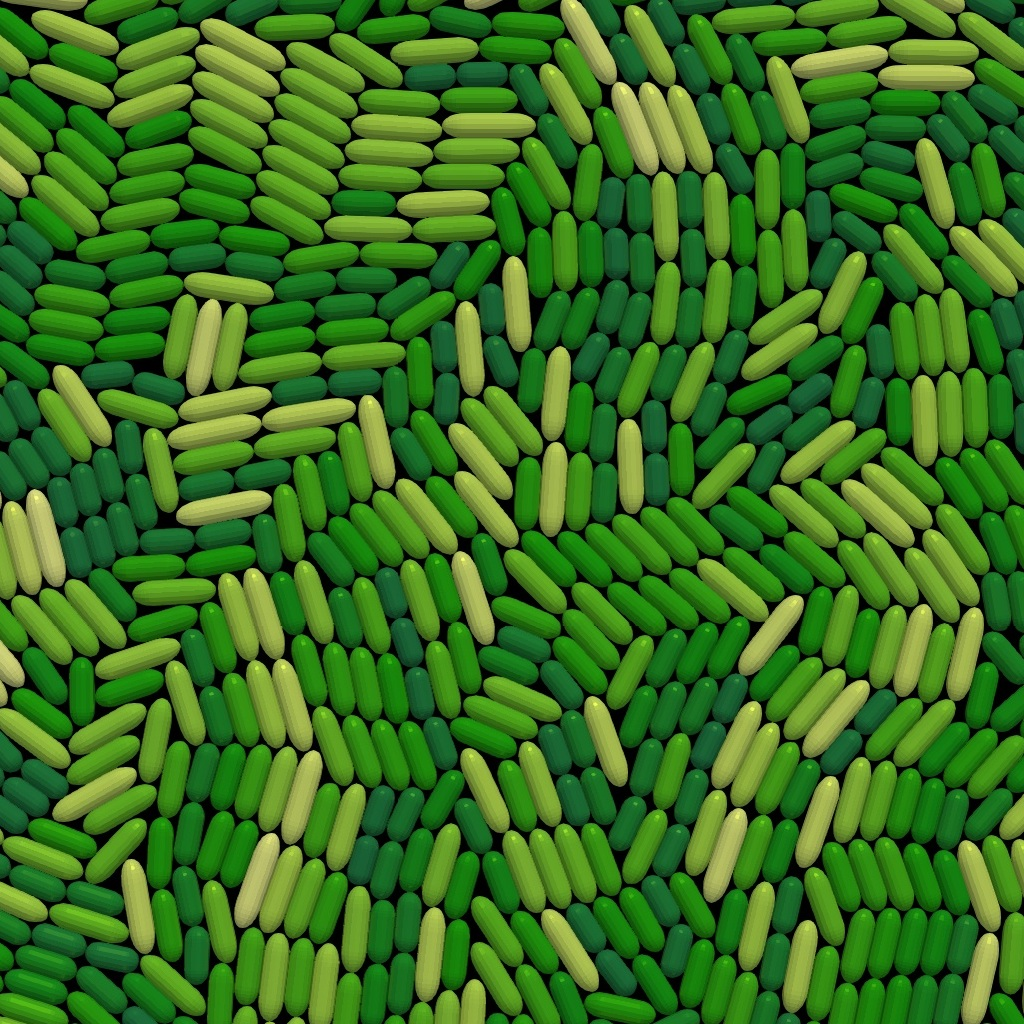
\includegraphics[width=\linewidth]{figures/comparison_plots/density_hard.jpeg}
        \caption{Close-up of particle packing for the hard model.}
        \label{fig:packing_hard}
    \end{subfigure}
    \begin{subfigure}[b]{0.49\columnwidth}
        \centering
        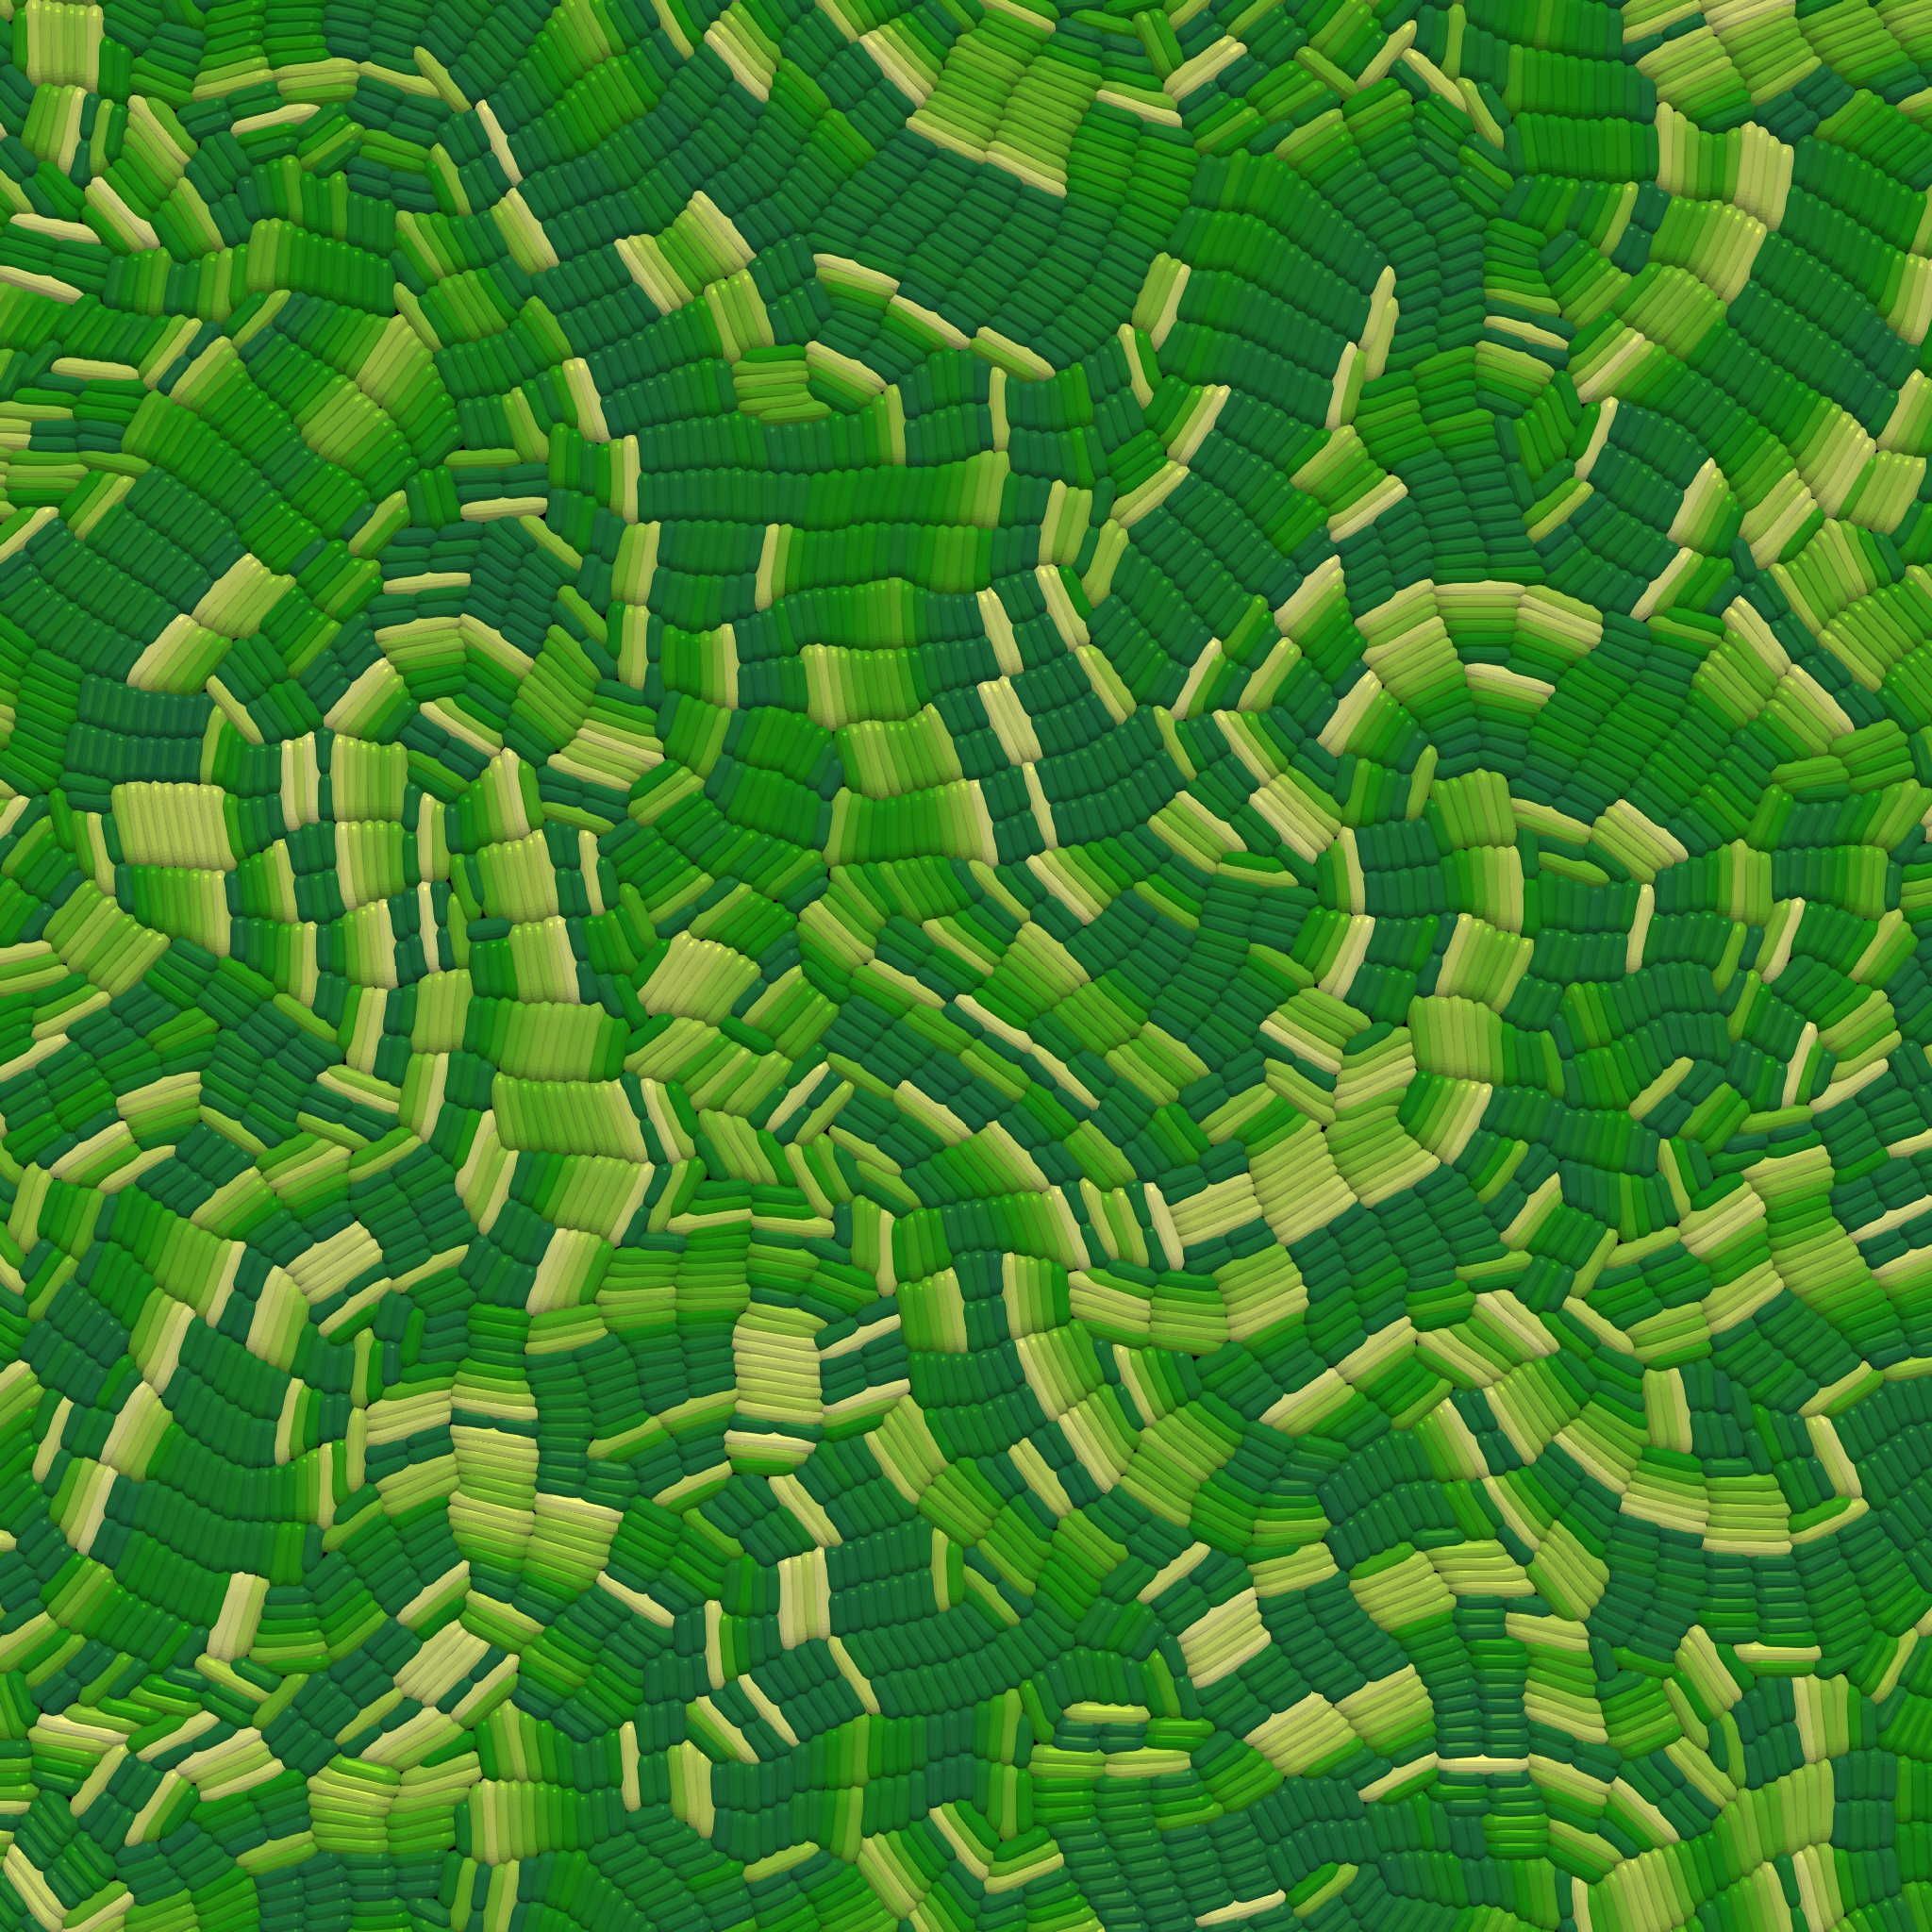
\includegraphics[width=\linewidth]{figures/comparison_plots/density_soft.jpeg}
        \caption{Close-up of particle packing for the soft model.}
        \label{fig:packing_soft}
    \end{subfigure}
    \caption{Close-up comparison of particle packing. The soft model exhibits denser packing with slight particle overlap, while the hard model maintains strict non-overlap. See \autoref{fig:radial_distribution_packing_fraction} for a quantitative comparison of packing fractions.}
    \label{fig:dense_packing_comparison}
\end{figure}


\begin{figure}[h]
    \centering
    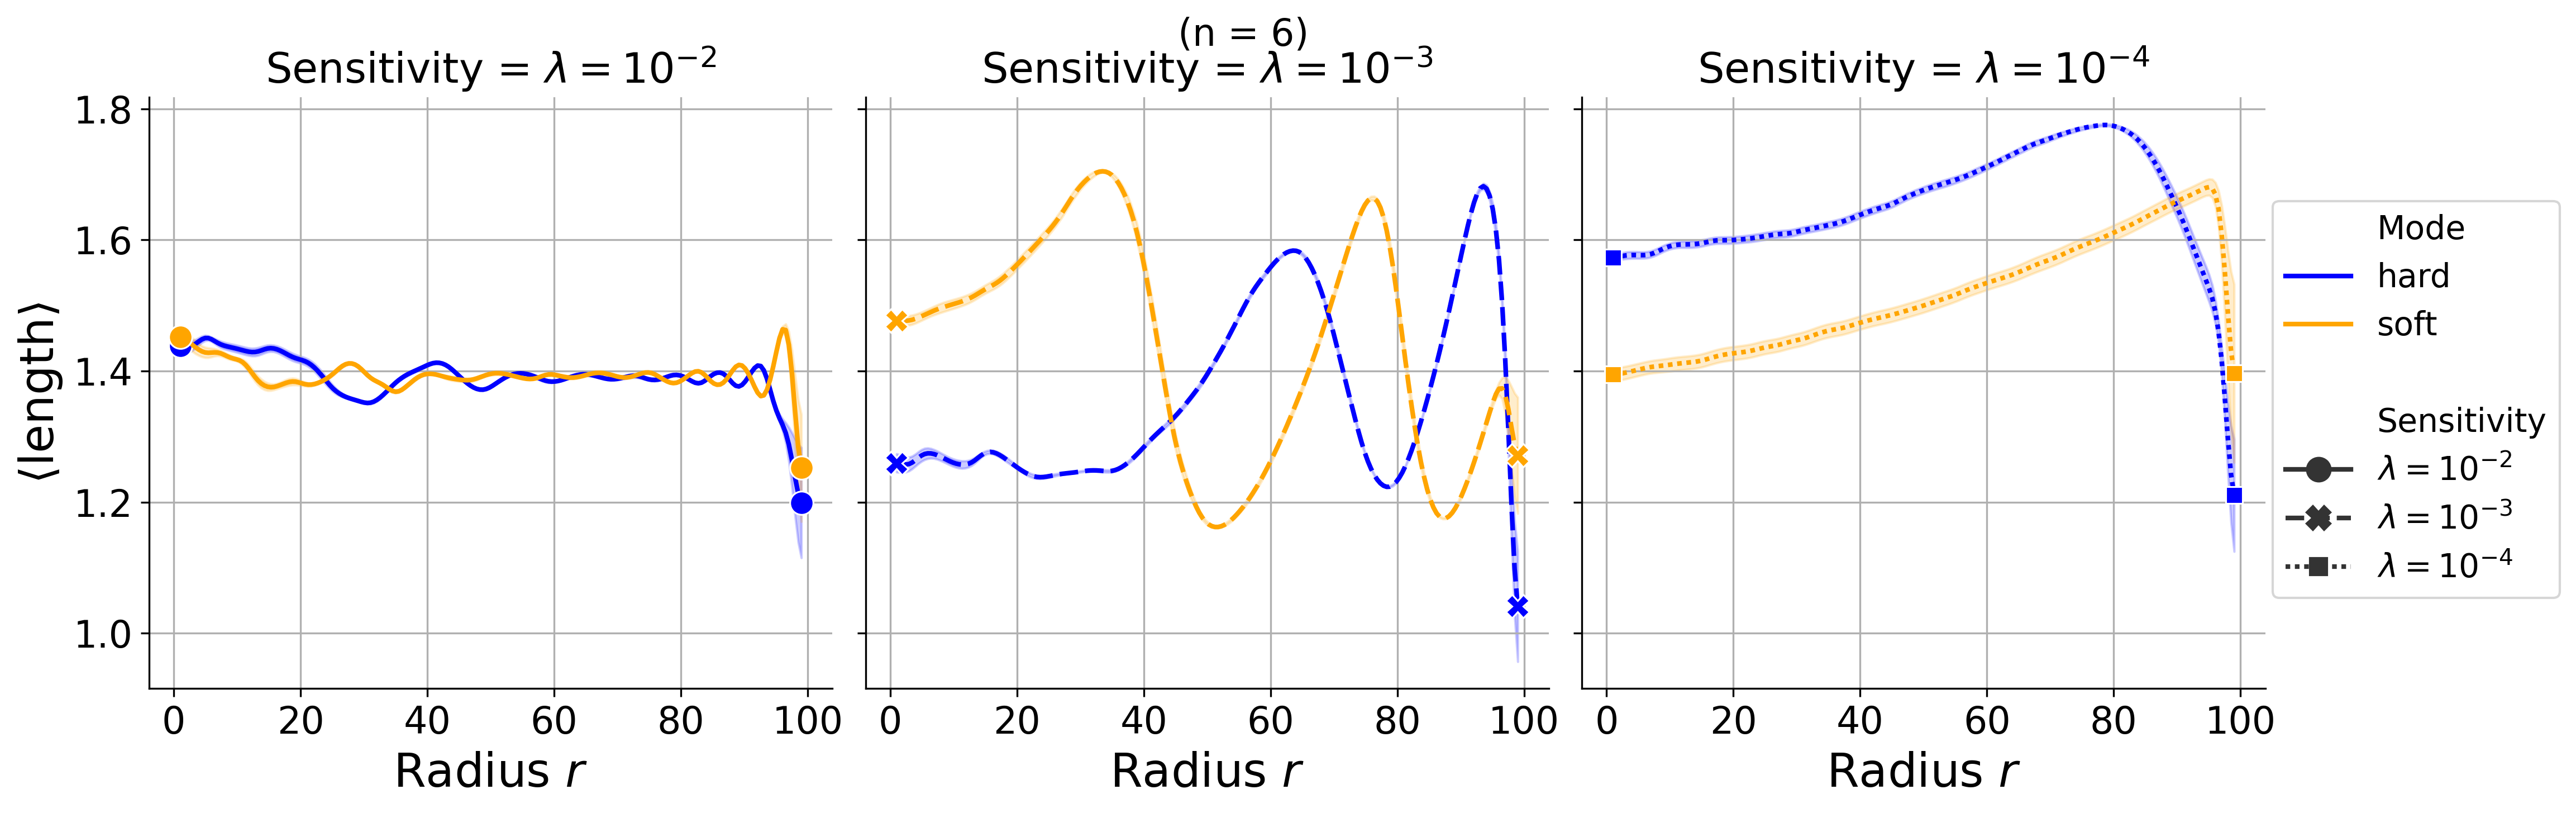
\includegraphics[width=\linewidth]{figures/comparison_plots/combined_length_shared.png}

    \caption{ }
\end{figure}


\begin{figure}[h]
    \centering
    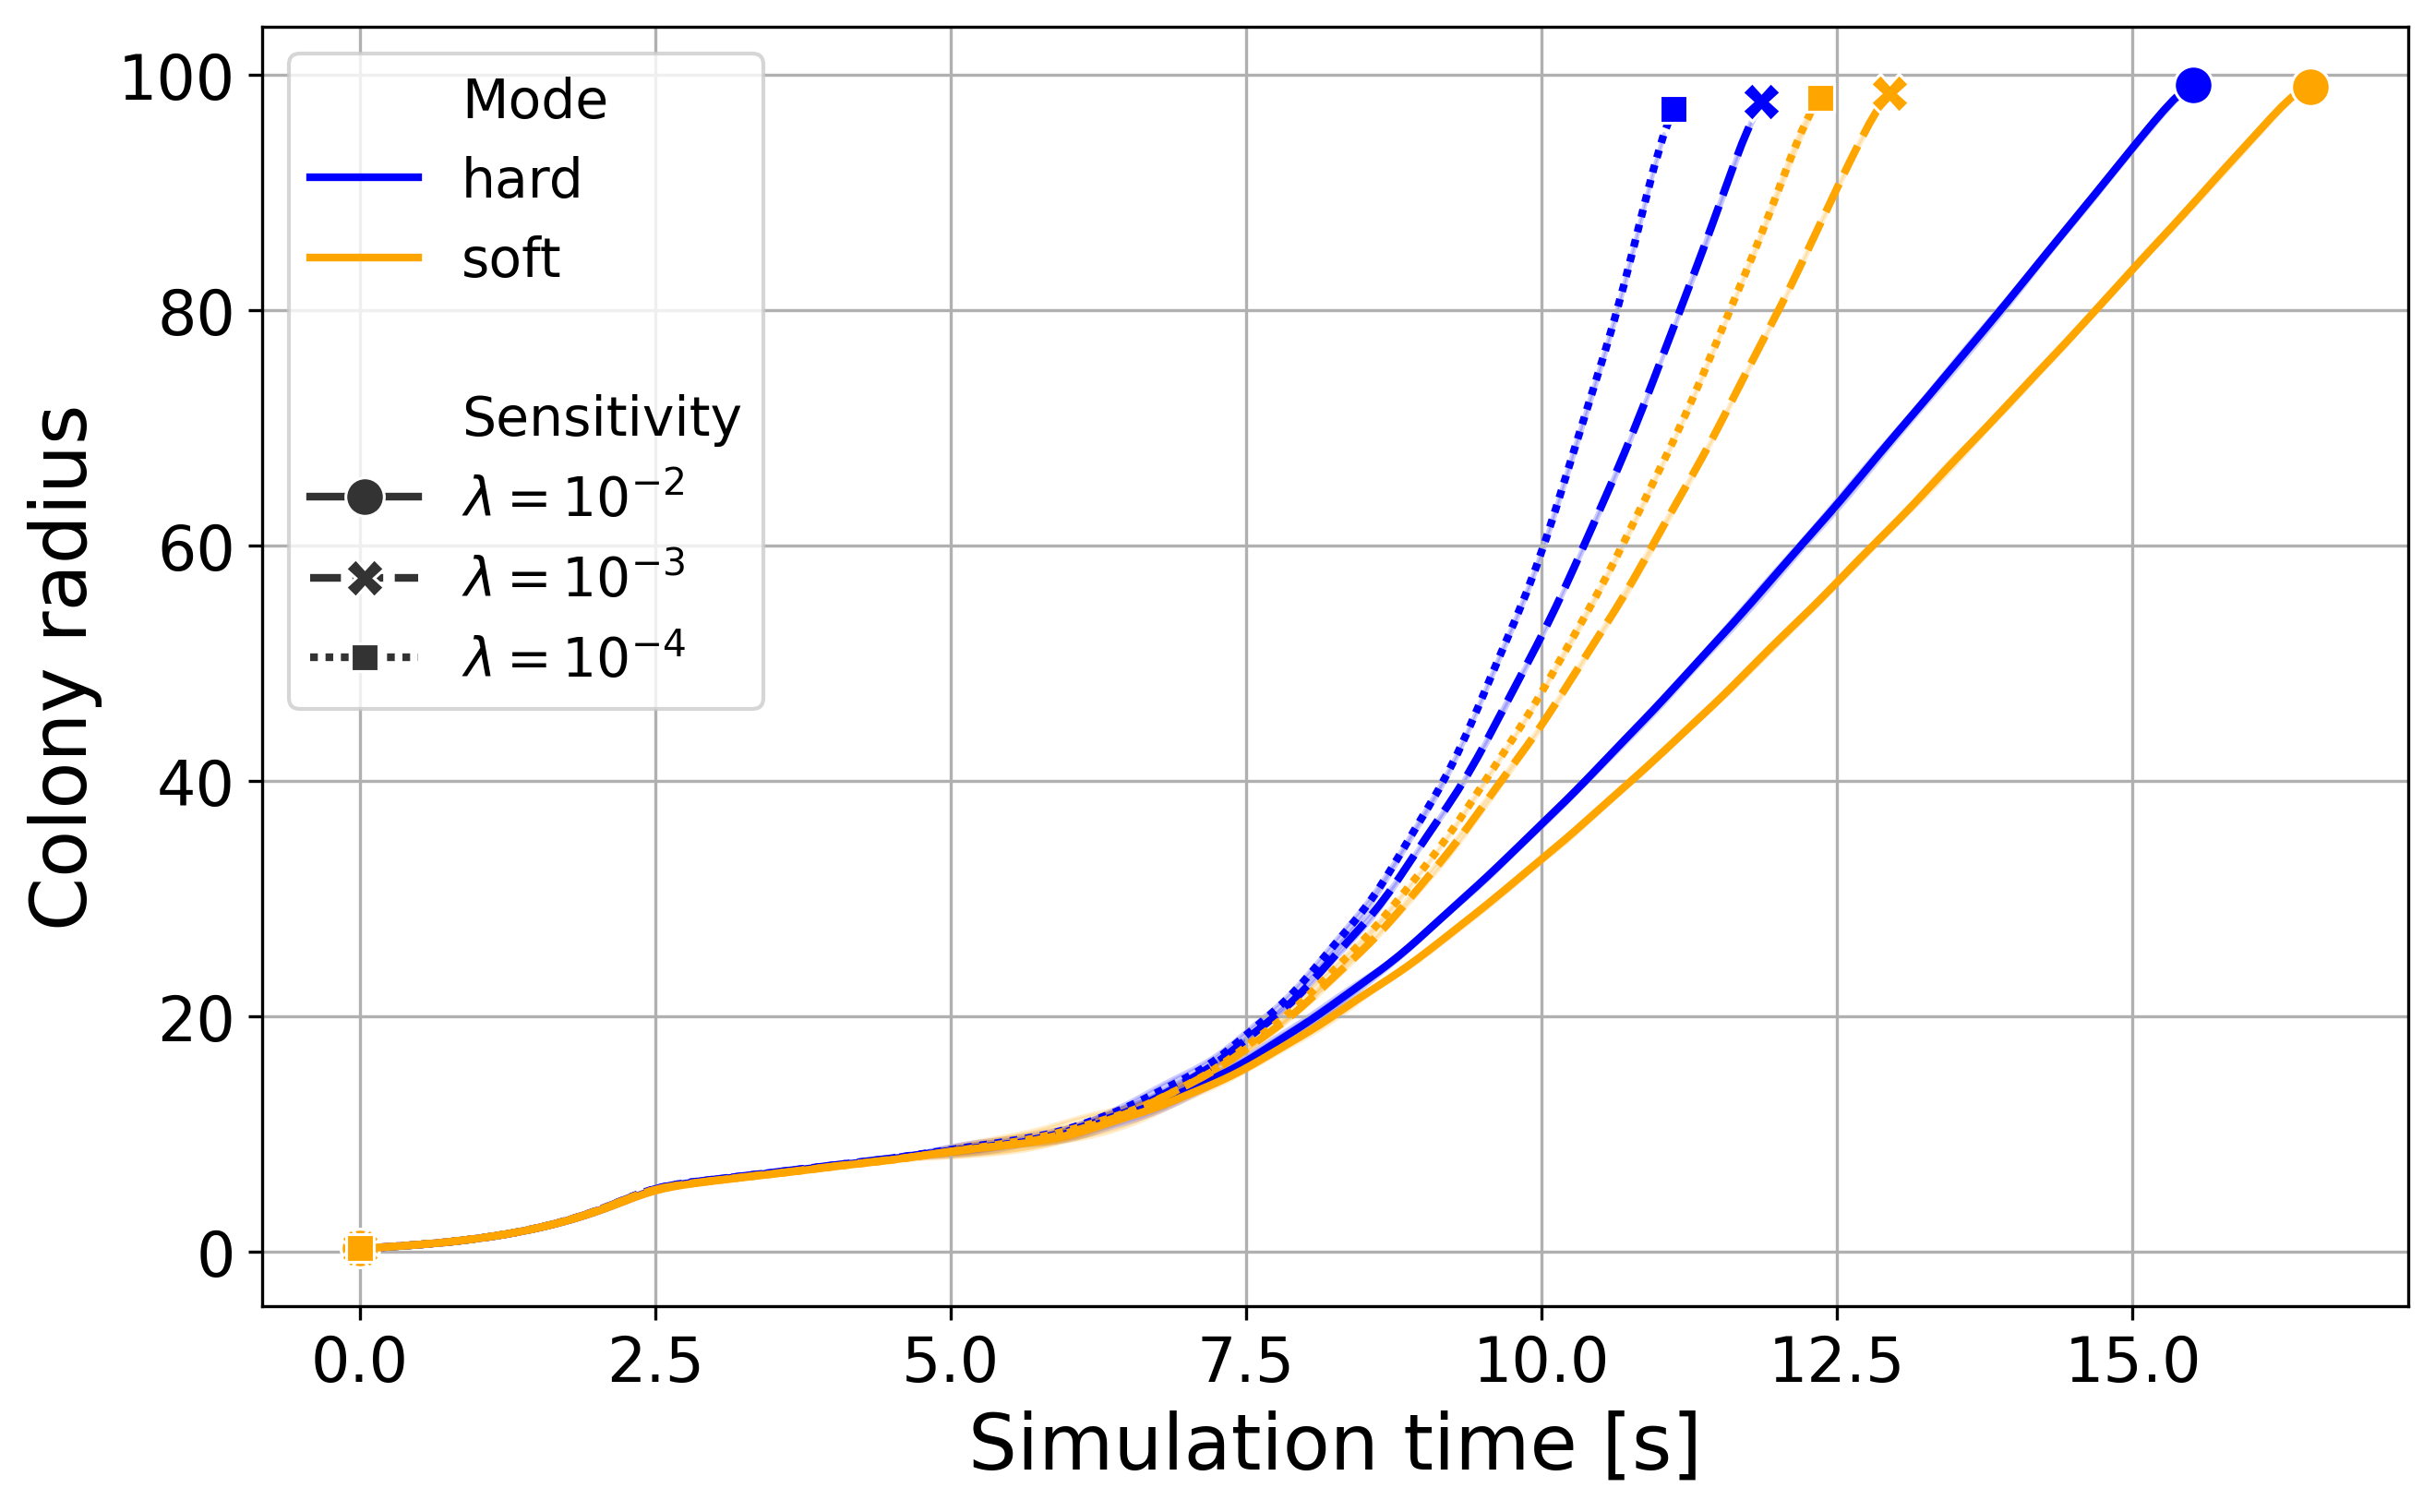
\includegraphics[width=\linewidth]{figures/comparison_plots/combined_simulation_time [s]_vs_colony_radius.png}
    \caption{ }
\end{figure}

\begin{figure}[h]
    \centering
    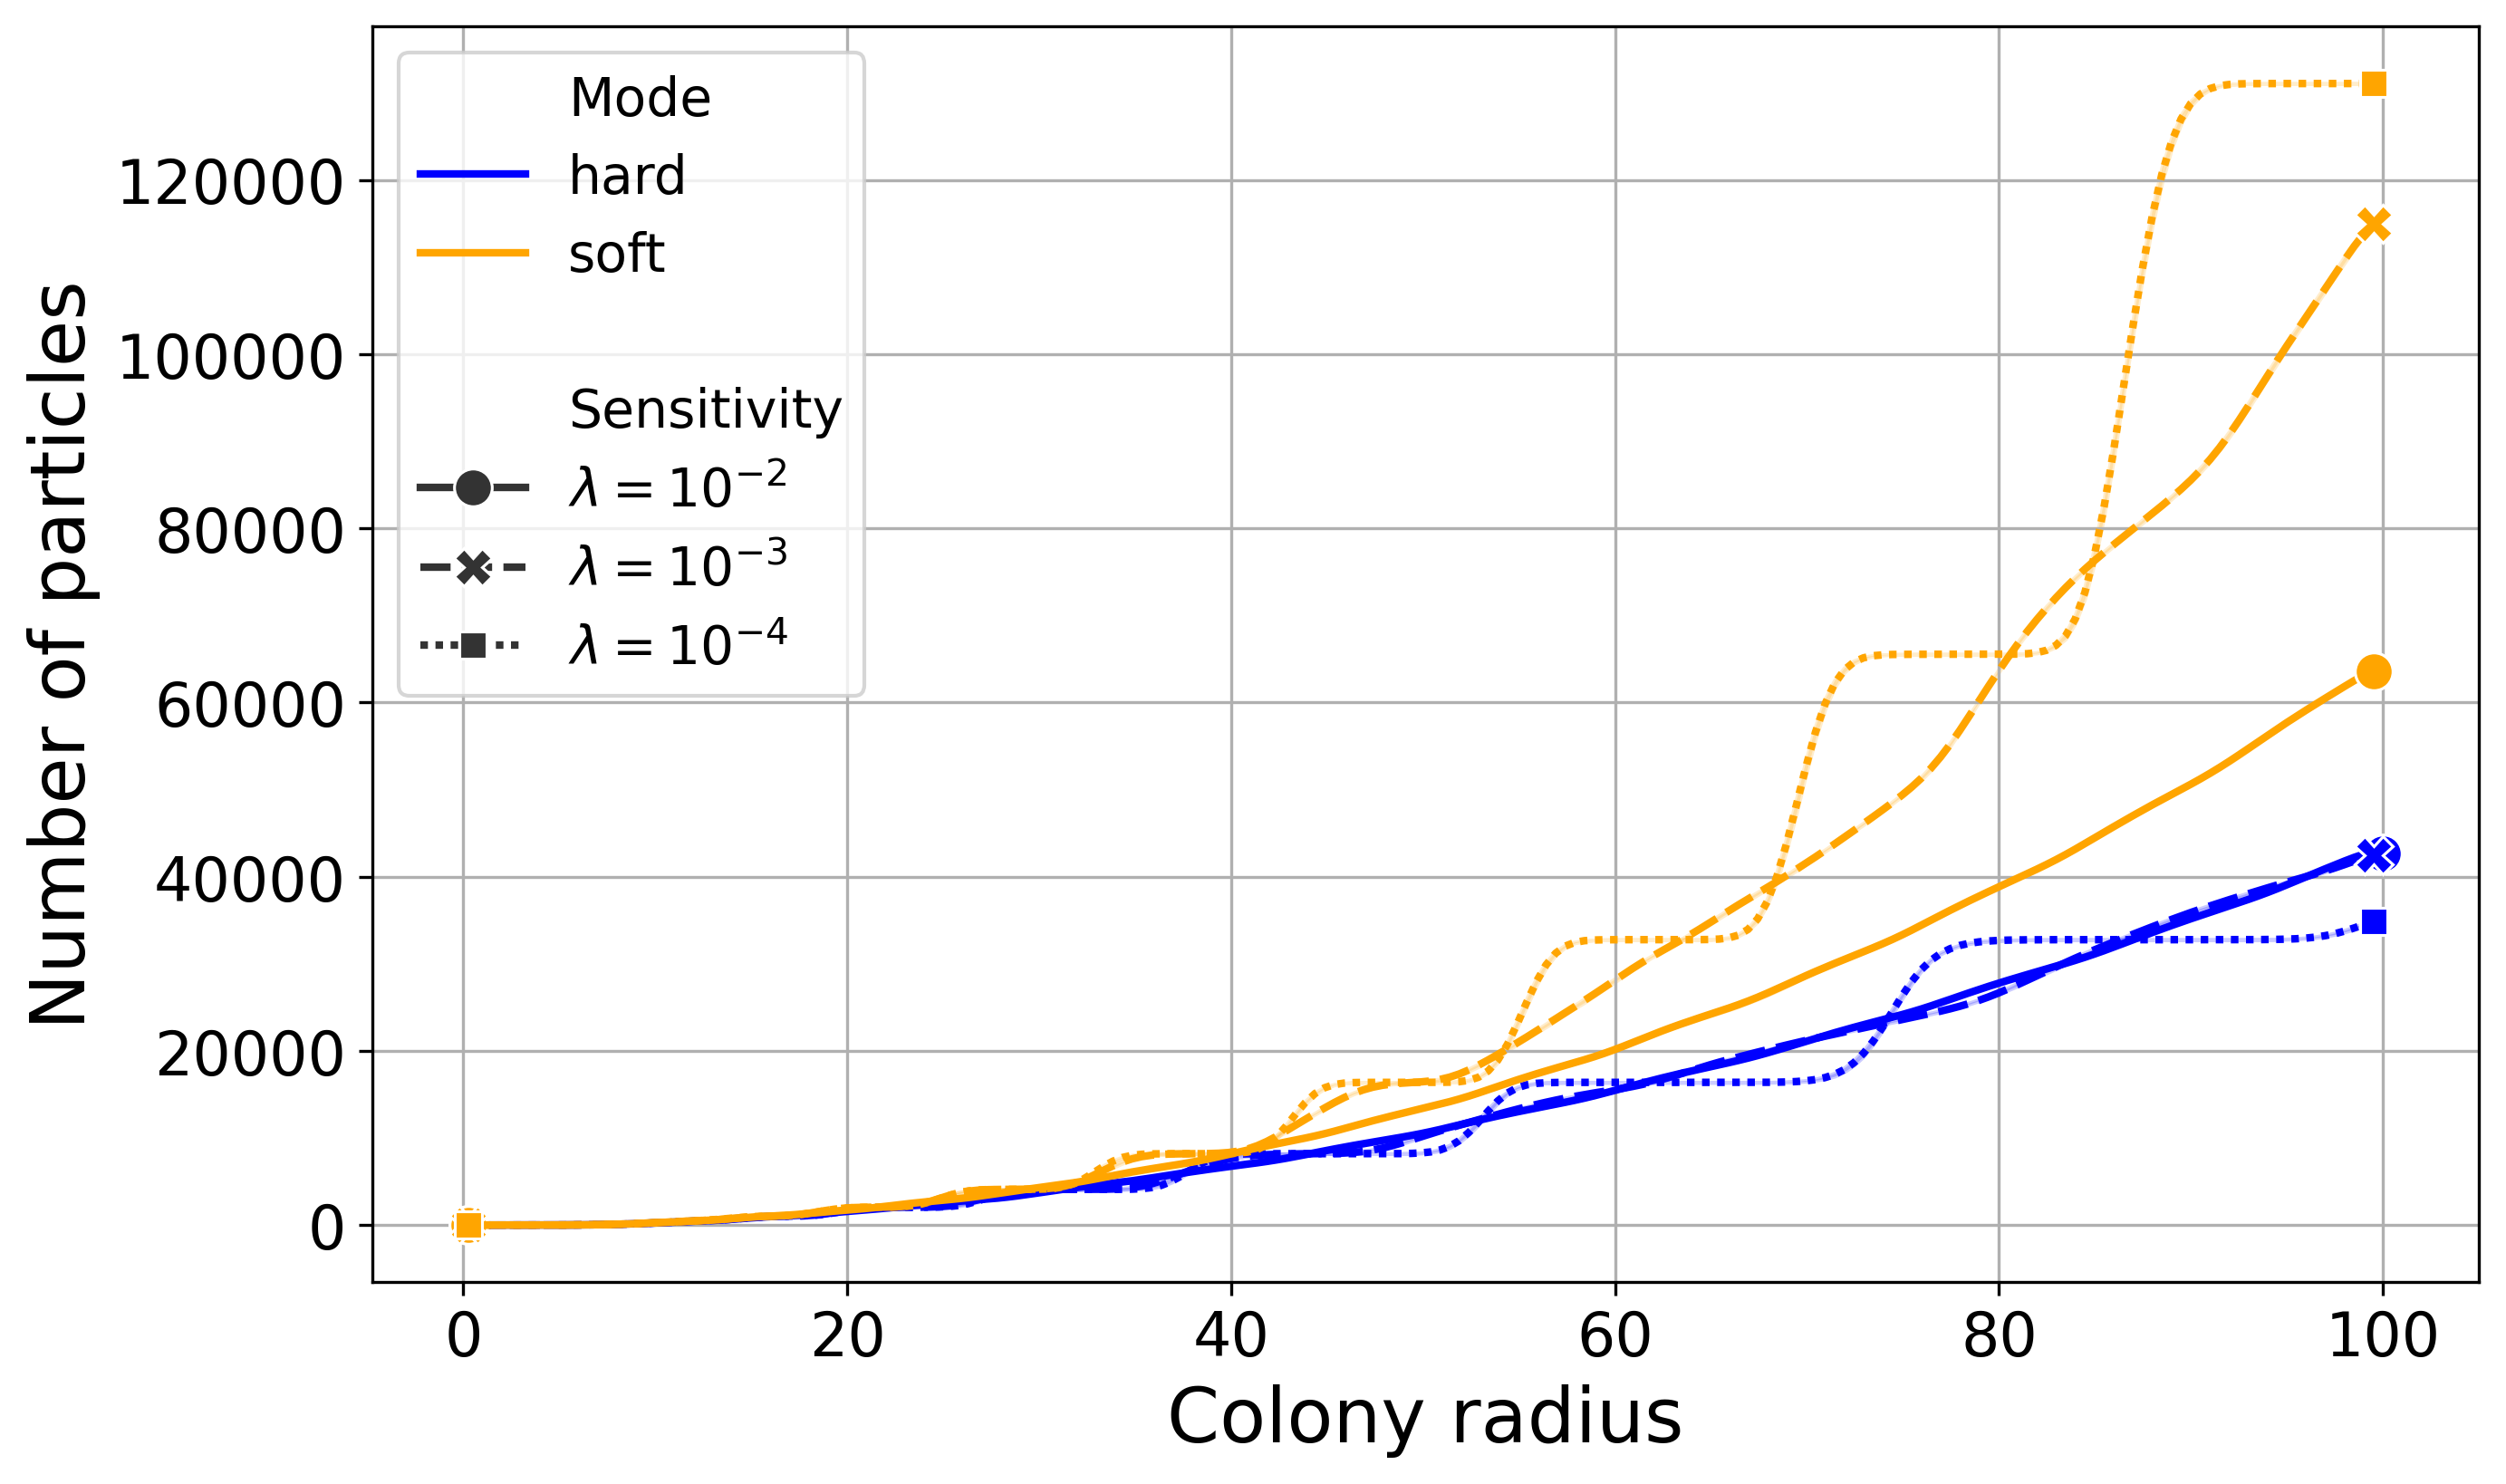
\includegraphics[width=\linewidth]{figures/comparison_plots/combined_colony_radius_vs_num_particles.png}
    \caption{ }
\end{figure}

\newpage

\begin{figure}[H]
    \centering
    \begin{subfigure}[b]{\linewidth}
        \centering
        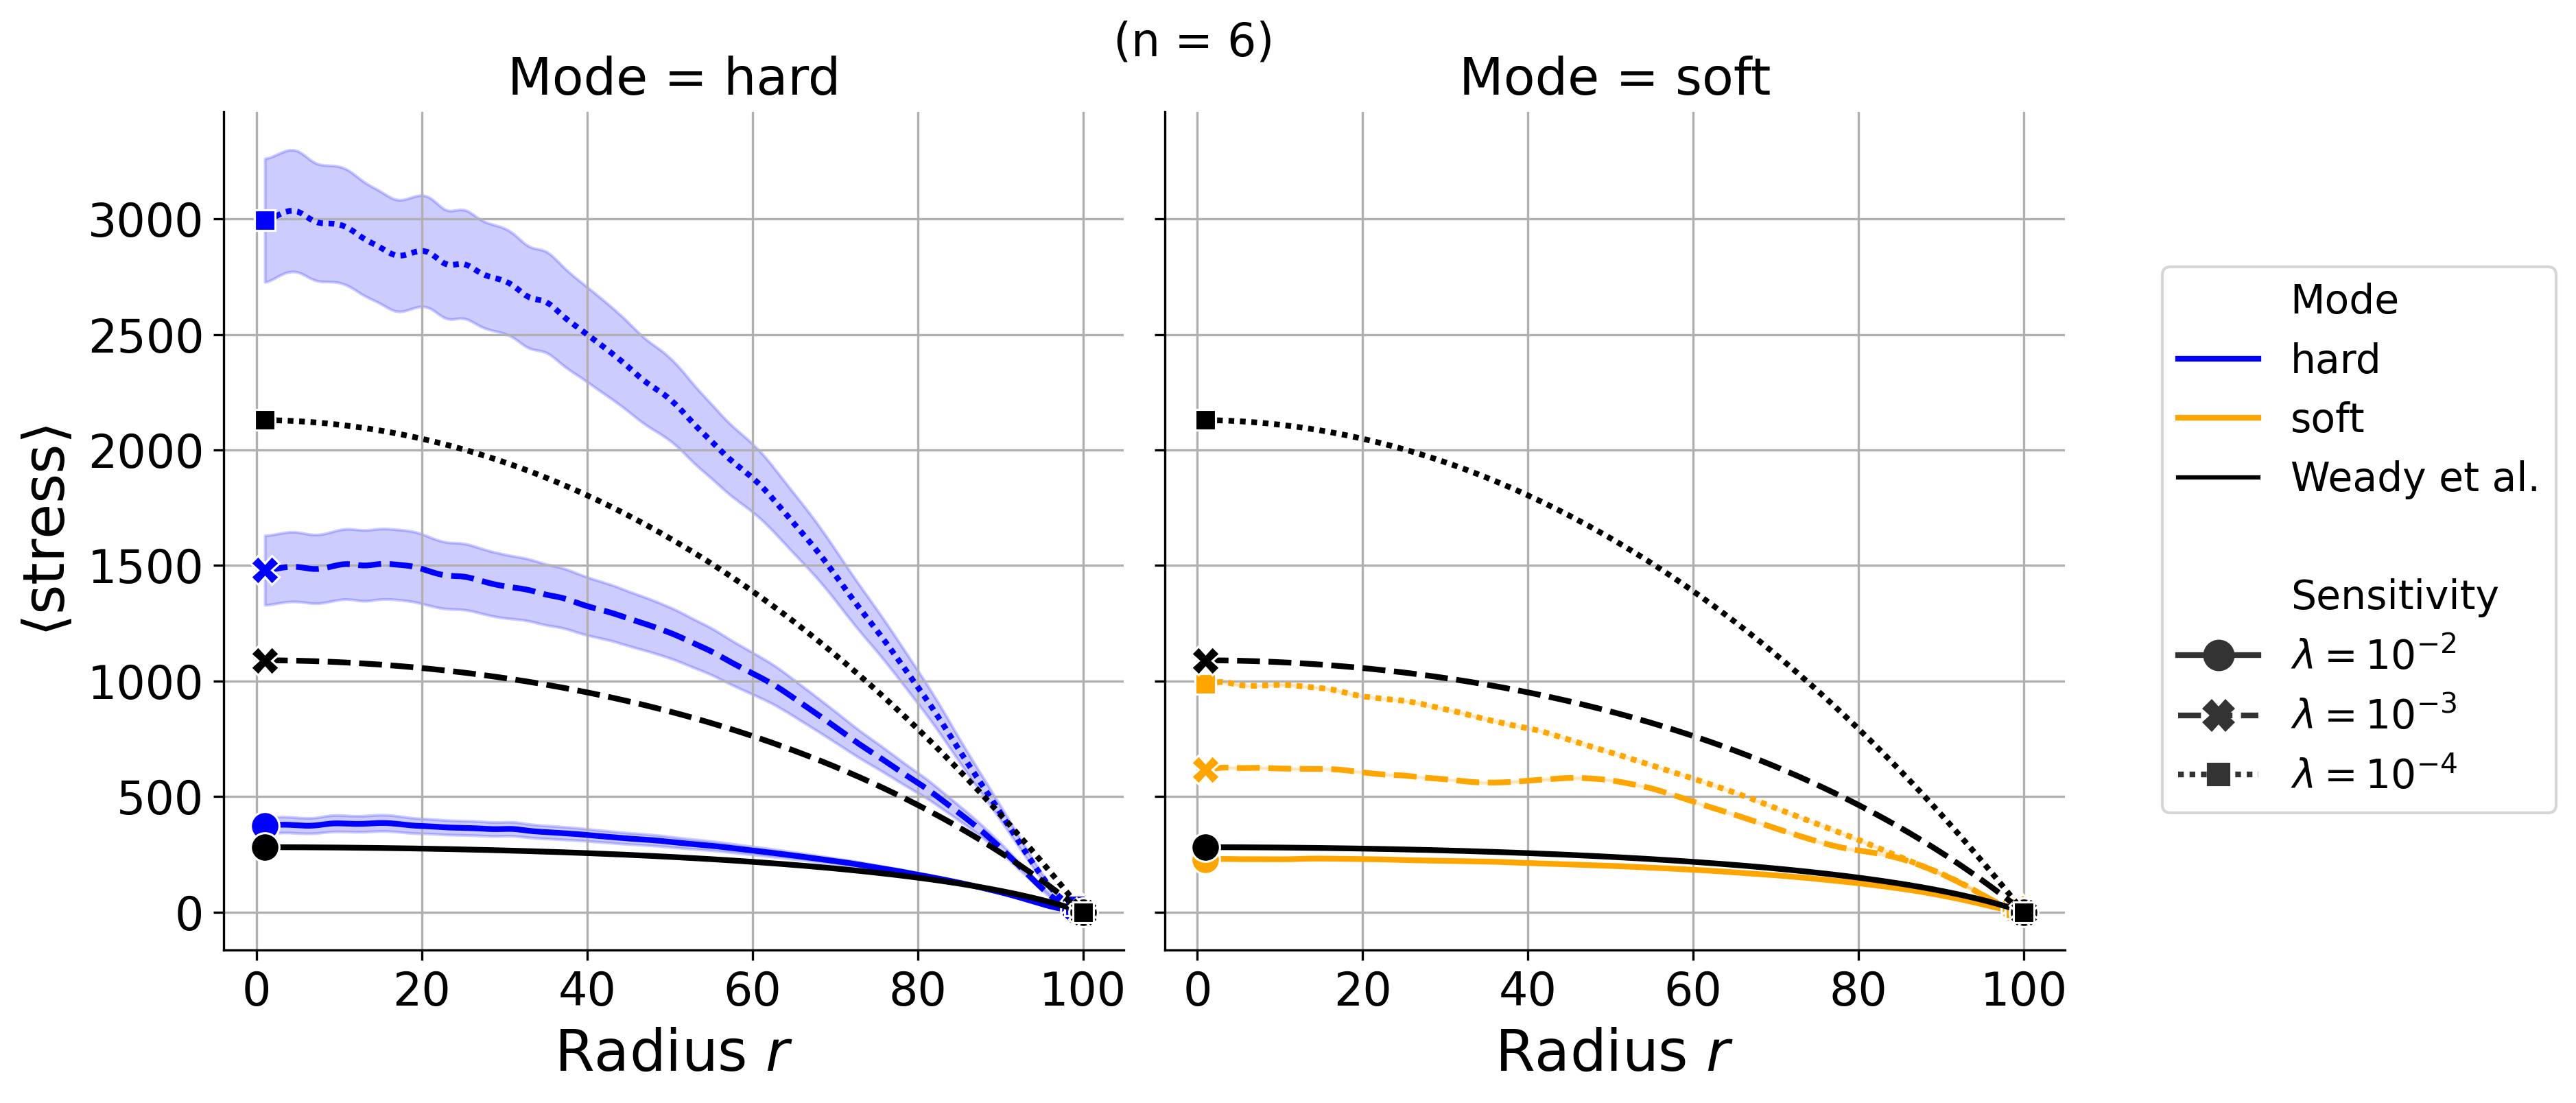
\includegraphics[width=\linewidth]{figures/comparison_plots/combined_stress_shared.png}
        \caption{Comparison of radial stress distributions for the hard and soft collision models. Both models roughly reproduce the analytically derived stress profiles~\cite{Weady2024}.}
        \label{fig:radial_distribution_stress}
    \end{subfigure}

    \vspace{0.5em}

    \begin{subfigure}[b]{\linewidth}
        \centering
        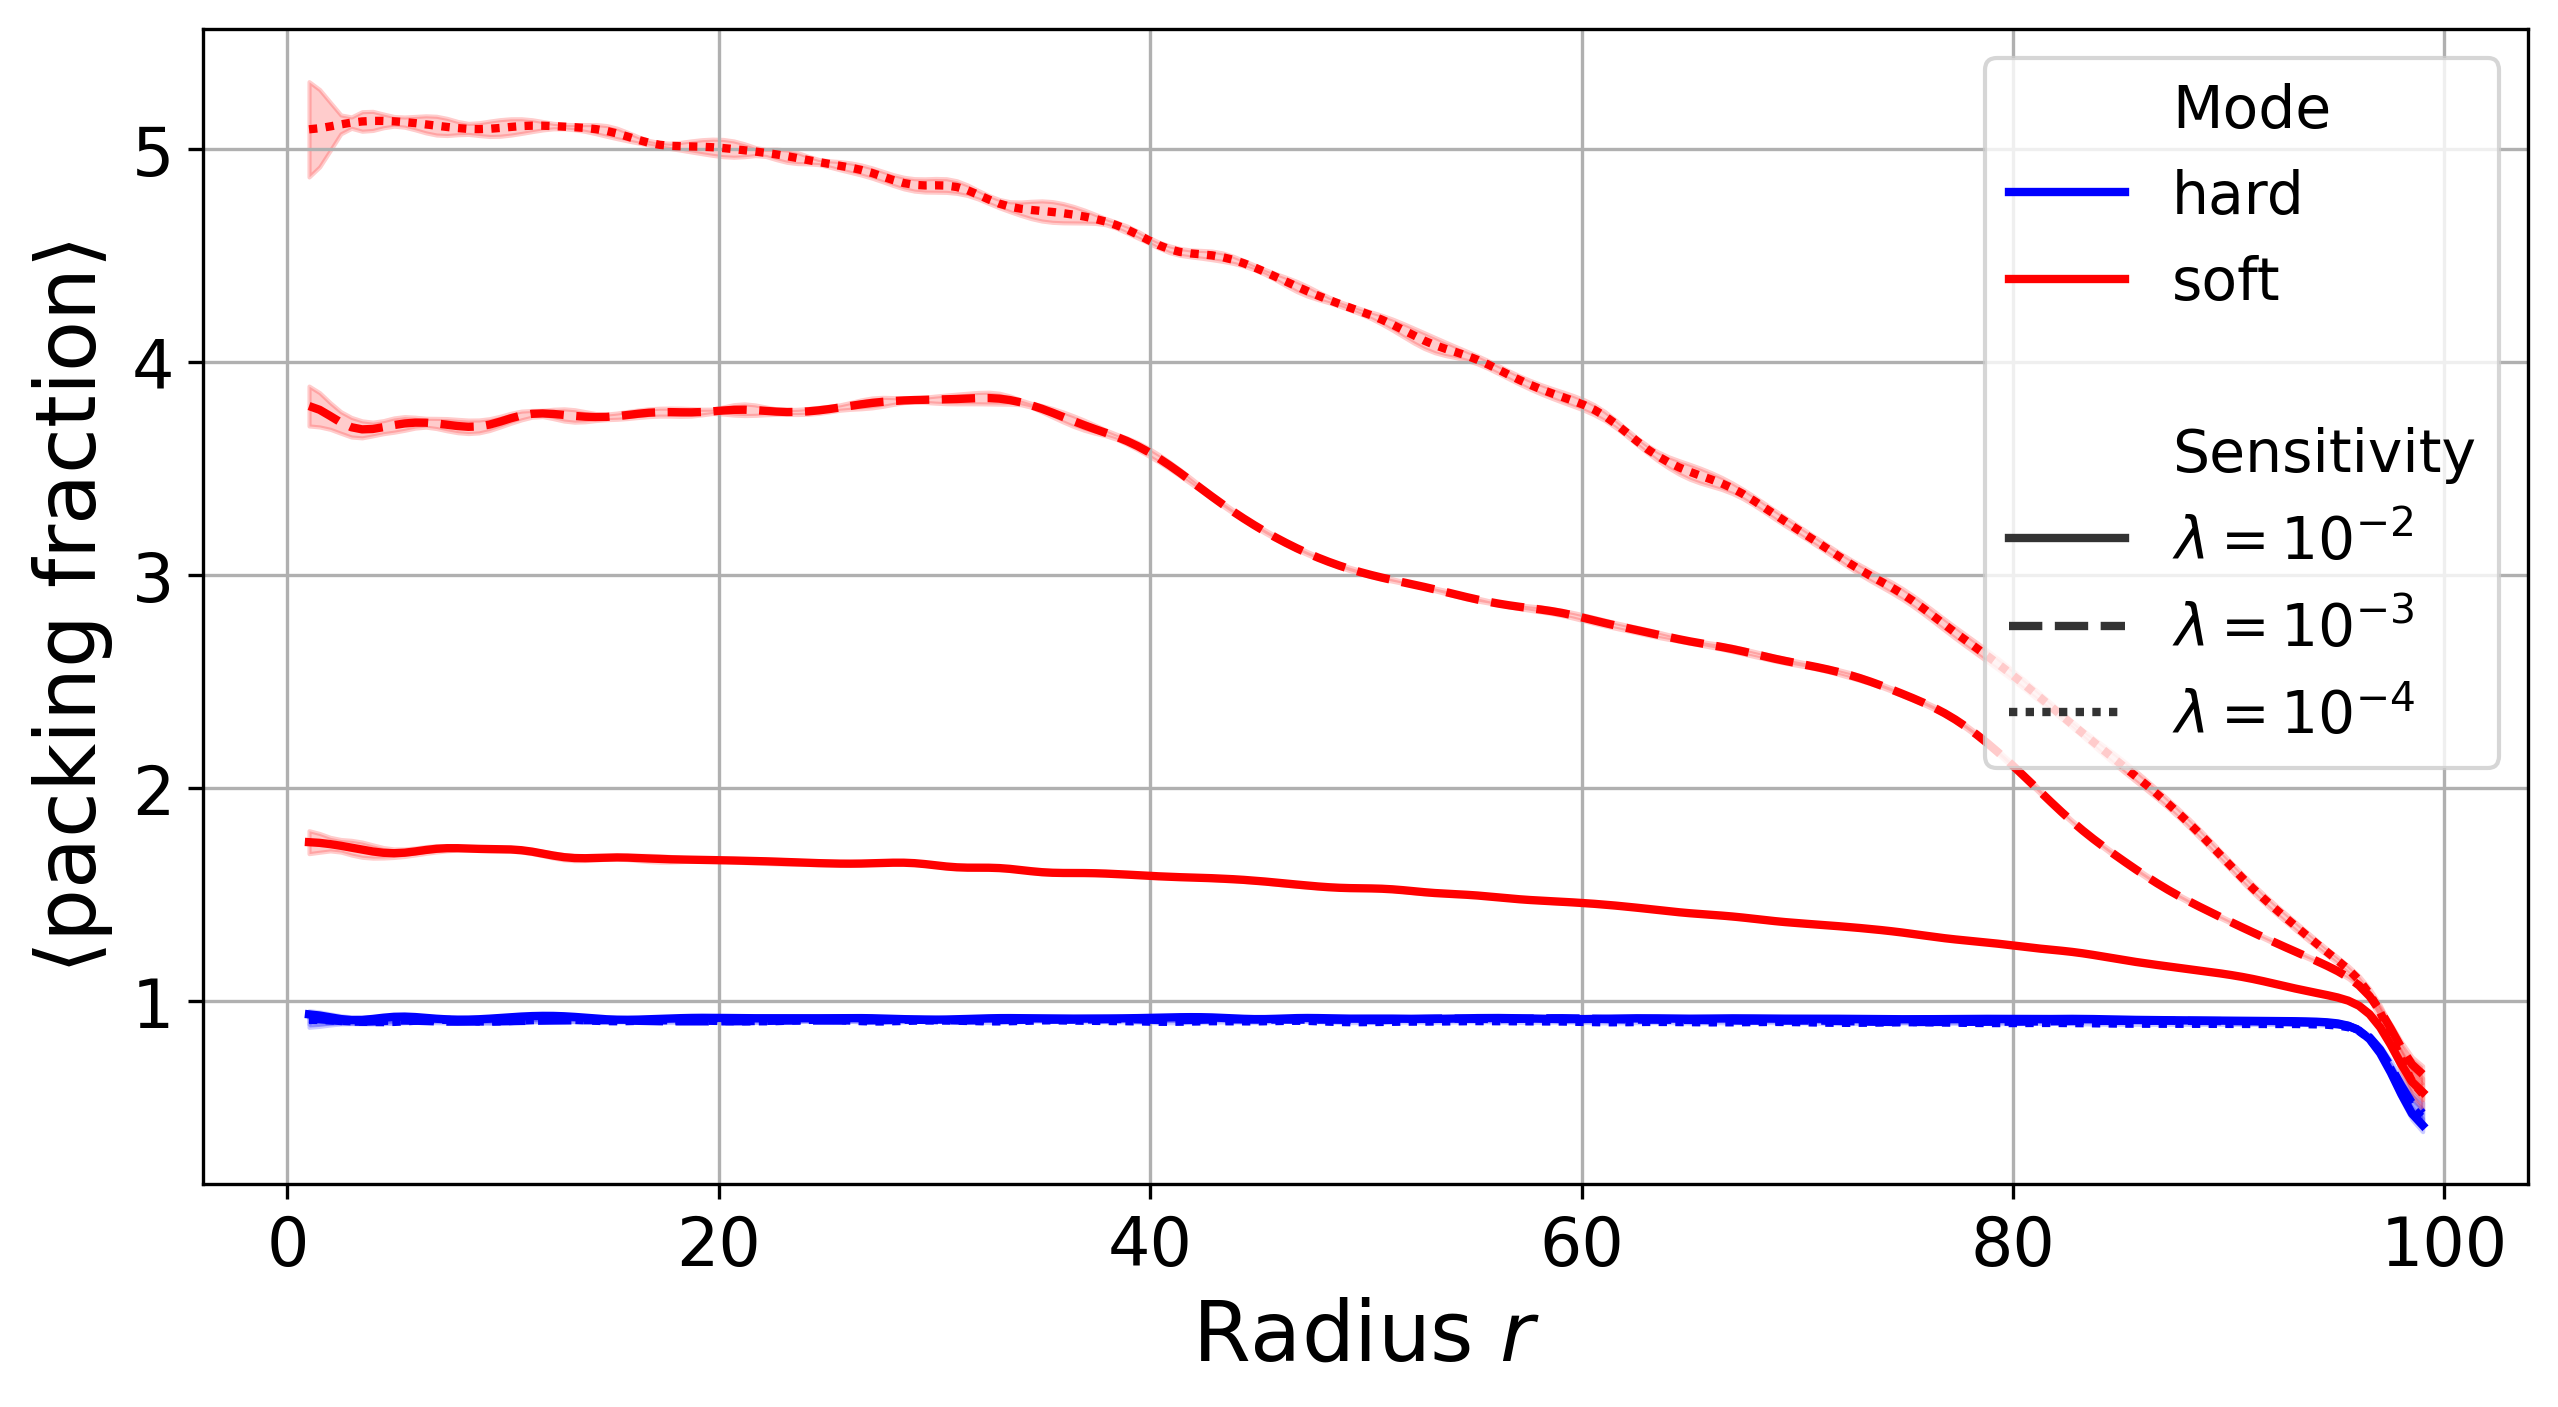
\includegraphics[width=\linewidth]{figures/comparison_plots/combined_radial_packing_fraction.png}
        \caption{Radial packing fraction. The soft model reaches $\approx1.2$ at the center due to overlap, while the hard model stays below 1. The packing fraction is defined as the total area occupied by particles within a radial shell divided by the shell area.}
        \label{fig:radial_distribution_packing_fraction}
    \end{subfigure}

    \vspace{0.5em}

    \begin{subfigure}[b]{\linewidth}
        \centering
        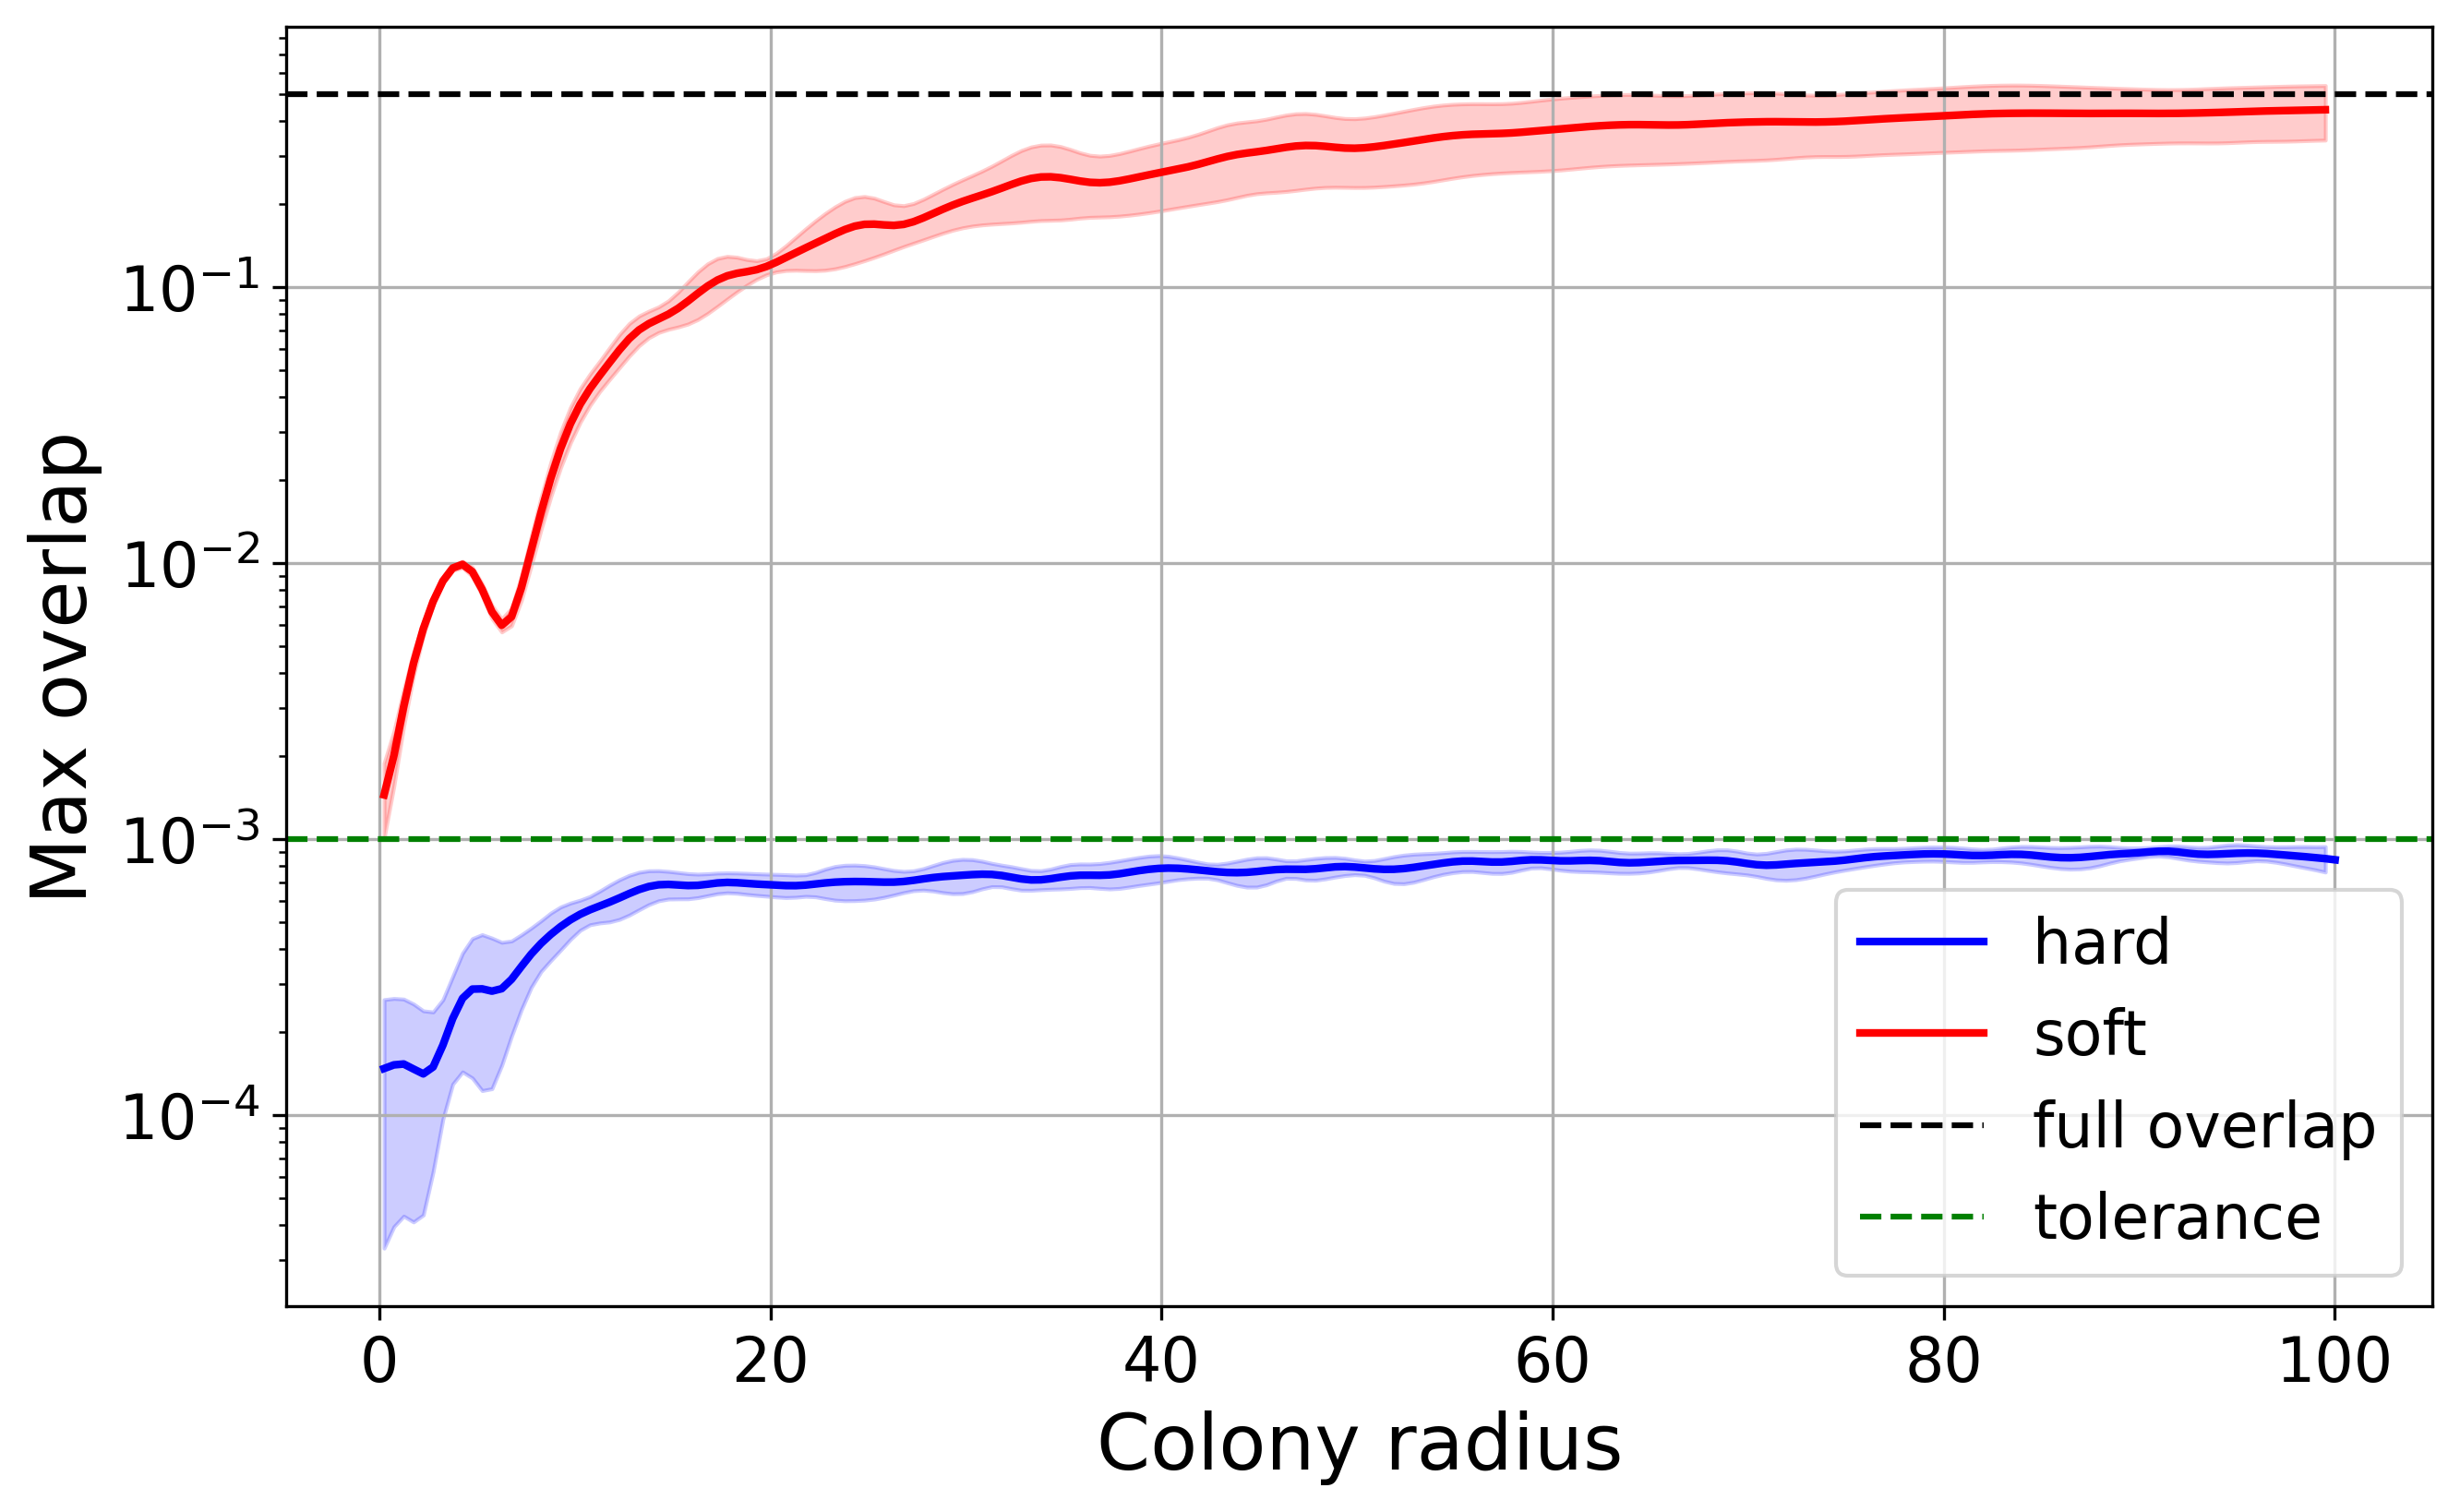
\includegraphics[width=\linewidth]{figures/comparison_plots/combined_colony_radius_vs_max_overlap_with_lines.png}
        \caption{Maximum particle overlap. Overlap grows over time in the soft model, while the hard model is kept near a constant value set by the tolerance hyperparameter.}
        \label{fig:max_overlap_simulation}
    \end{subfigure}

    \caption{Comparison of hard and soft collision models: (a) radial stress distributions, (b) radial packing fraction, and (c) maximum particle overlap.}
    \label{fig:comparison_all}
\end{figure}



\subsection{Microdommain formation}


Similar to You et al.~\cite{You2018,You_2021}, we can also observe the formation of microdomains of aligned cells within the colony. These domains emerge from mechanical interactions and growth dynamics, creating local regions where cells share similar orientations. As shown in \autoref{fig:orientation_comparison_small}, both hard and soft collision models capture this phenomenon for small colonies ($R \approx 50$) and are able to produce macroscopic patterns closely resembling the experimental observations of real \textit{E. coli} colonies as presented in~\cite{You2018}.

\begin{figure}[h]
    \centering
    \begin{subfigure}[b]{0.49\columnwidth}
        \centering
        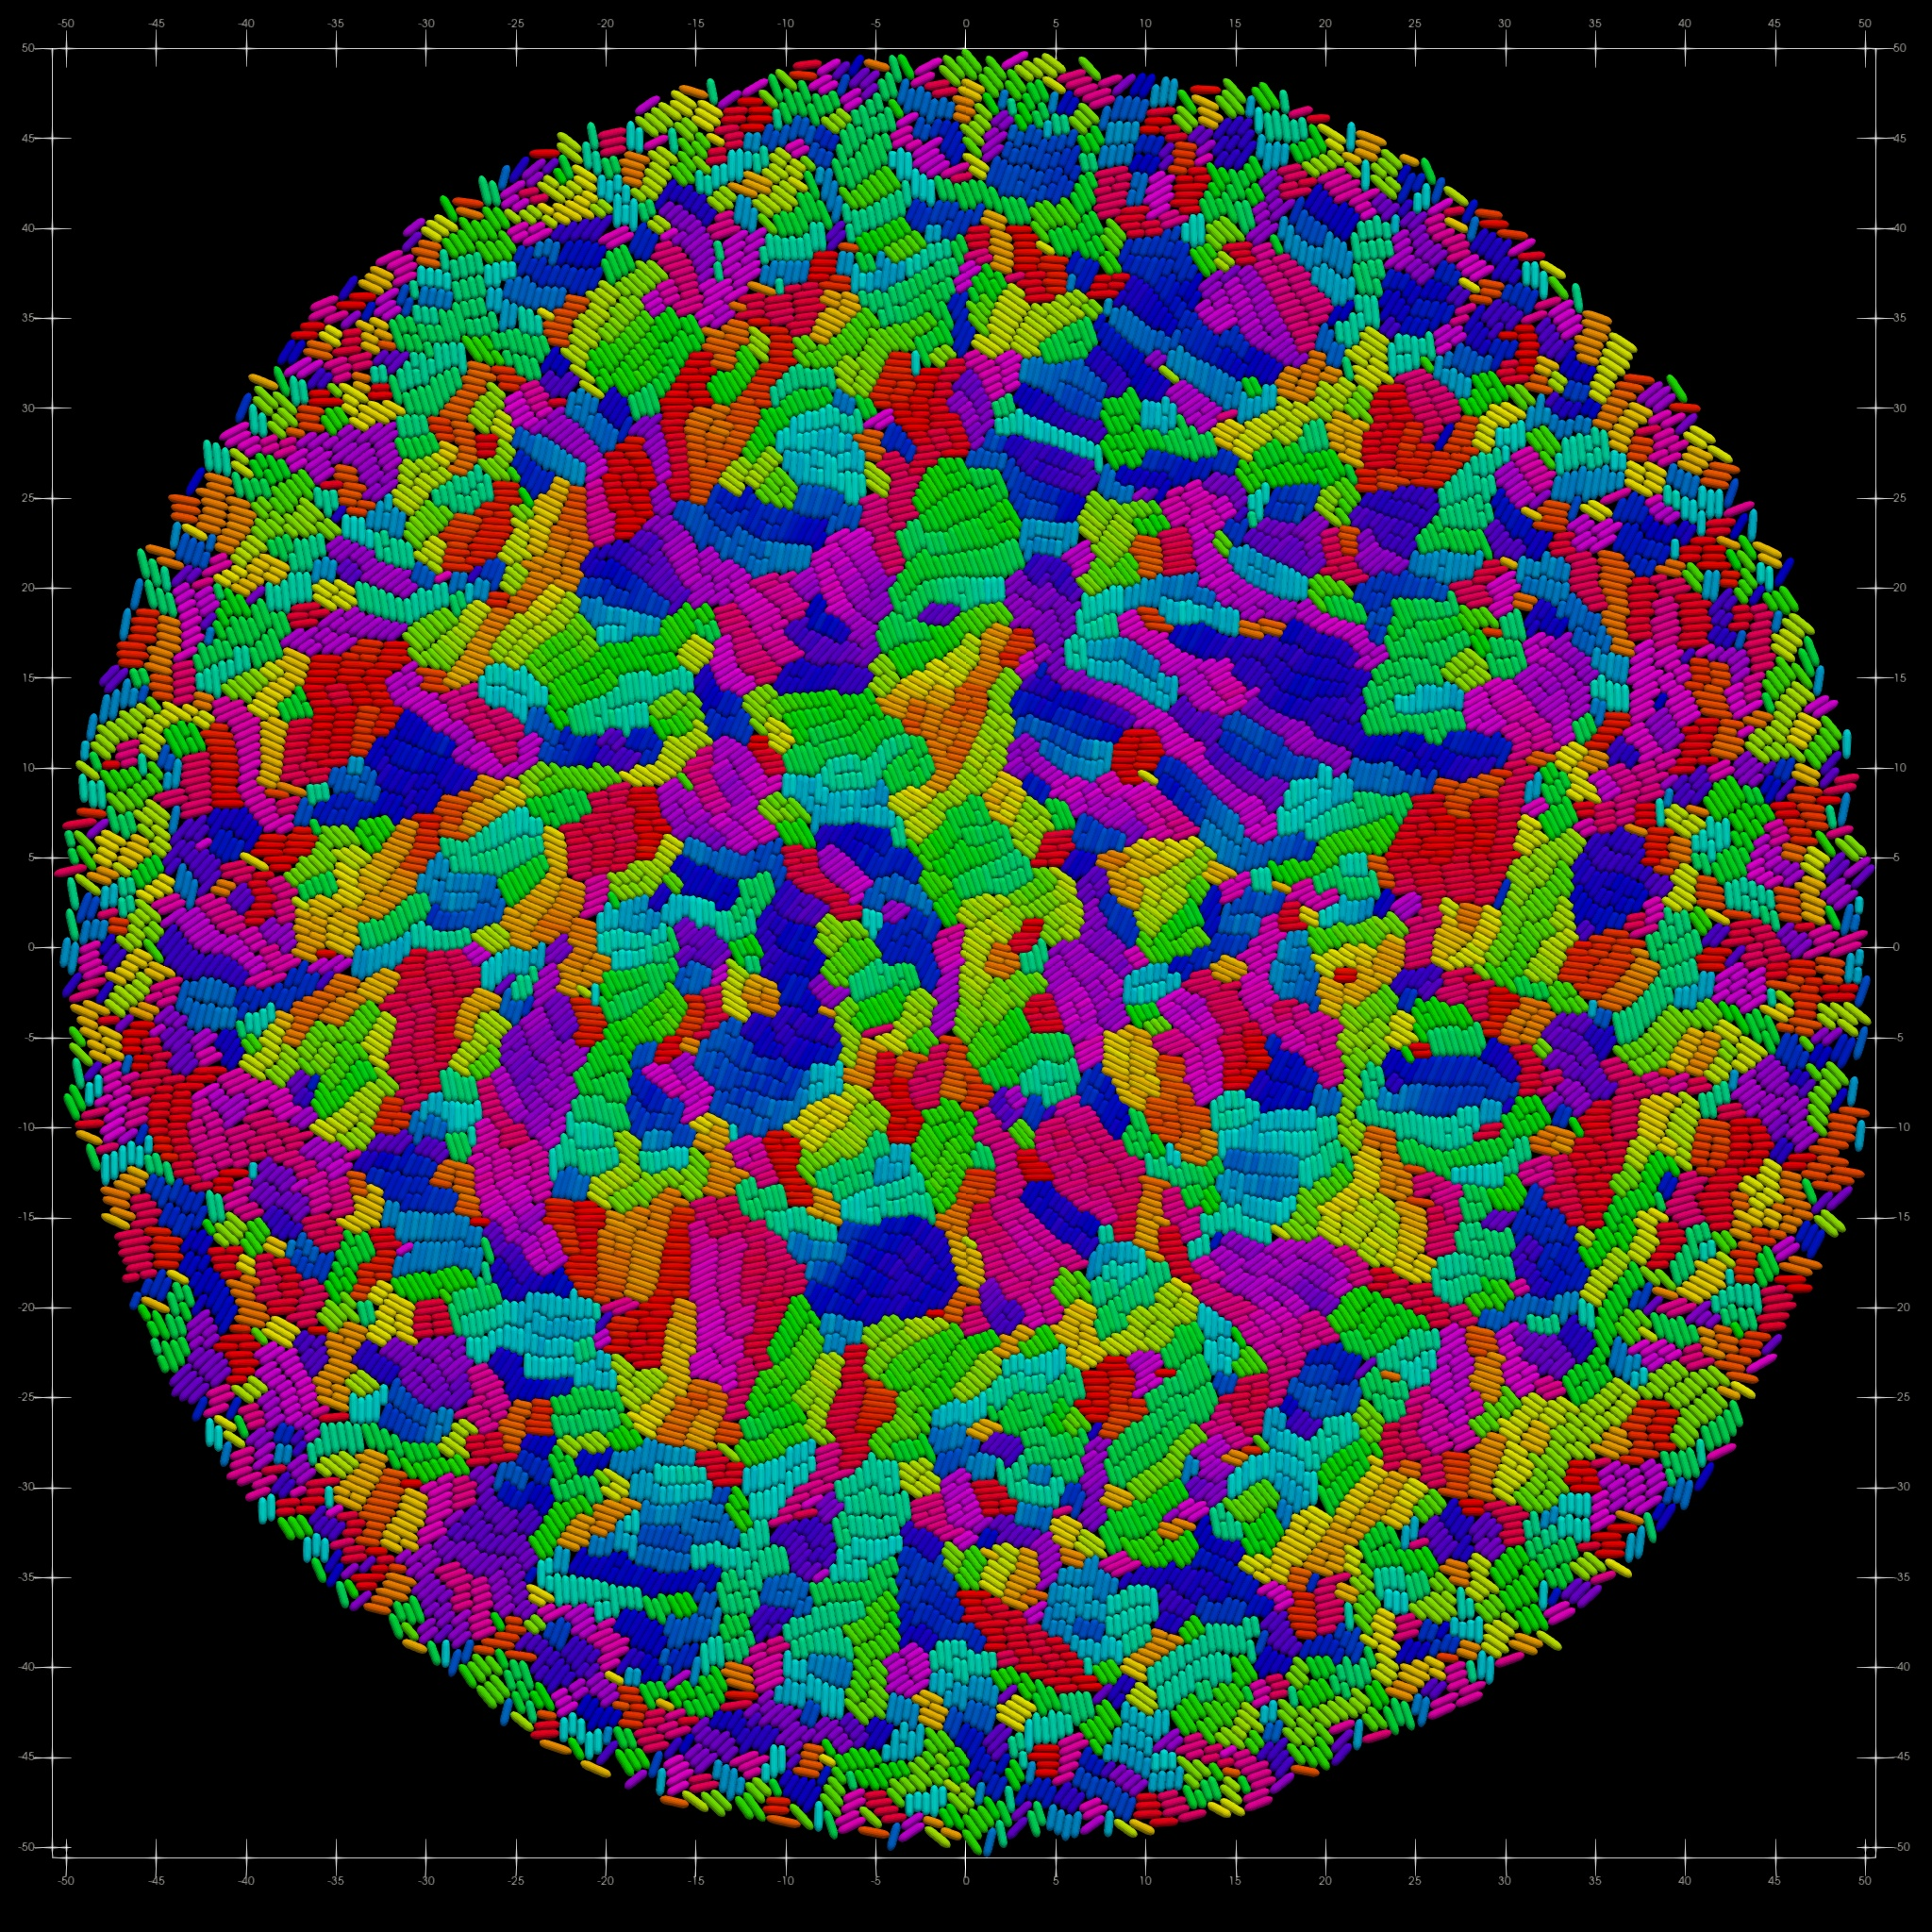
\includegraphics[width=\linewidth]{figures/orientation_comparisons/r50_soft_e-2.jpeg}
        \caption{Orientation pattern for the soft model at $R \approx 50$.}
        \label{fig:packing_hard}
    \end{subfigure}
    \begin{subfigure}[b]{0.49\columnwidth}
        \centering
        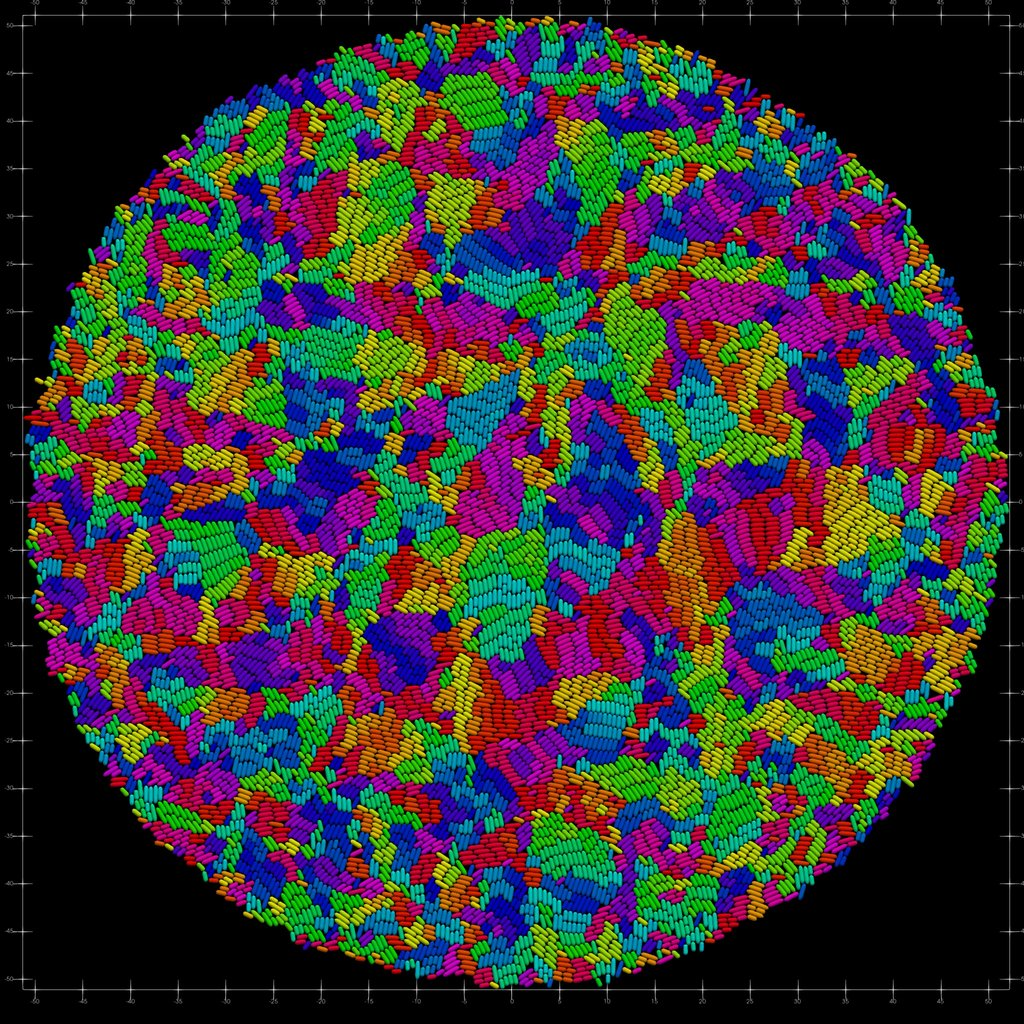
\includegraphics[width=\linewidth]{figures/orientation_comparisons/r50_hard_e-2.jpeg}
        \caption{Orientation pattern for the hard model at $R \approx 50$.}
        \label{fig:packing_soft}
    \end{subfigure}
    \caption{Comparison of orientation patterns for small colonies ($R \approx 50$) using the soft and hard collision models. Both models produce similar microdomain structures, closely matching experimental observations~\cite{You2018}.}
    \label{fig:orientation_comparison_small}
\end{figure}

However the differences between the two models become more pronounced as the colony grows larger or the stress sensitivity parameter $\lambda$ decreases. As shown in \autoref{fig:orientation_comparison}, the hard model tends to produce distinct and similar patches of aligned cells for all values of $\lambda$, whereas the soft model often results in elongated, unrealistic, bundles of aligned, densely packed cells. This artefact, is directly caused by the soft model not being able to prevent overlaps completely, causing the interior of the colony to become unrealistically dense.

Therfore, the soft model is not suitable for studying microdomain formation in large colonies or at low stress sensitivities, but is a viable and easier-to-implement alternative studying macroscopic pattern formation in smaller colonies of up to radius $R \approx 50$, such as those presented in~\cite{You2018}.

The hard model's strict non-overlapping constraints prevent cells from clustering too closely, leading to a highly realistic structure at all colony sizes, clearly resembling experimental observations.



\clearpage
\newpage



\section{Computational Performance}

Both models reproduce the observed patterns, but their computational requirements differ substantially. The hard collision model requires solving a gradient-based optimization problem at each time step, whereas the soft collision model relies on inexpensive direct force calculations. This creates a trade-off between per-step cost, maximum stable time step, and overall simulation time. In the following sections, we analyze these aspects in detail.

\subsection{Critical Time Step}

The soft collision model is cheaper per interaction but typically requires smaller integration time steps to maintain numerical stability due to the stiffness of the repulsive forces. In contrast, the hard collision model can often operate with larger time steps since it enforces non-overlap constraints directly, although its per-step cost is significantly higher because of the global optimization problem.

\autoref{fig:simulation_time_vs_dt} shows the maximum stable time step $\Delta t$ for both models during a simulation. The optimal time is determined by \autoref{alg:adaptive_dt}, which adjusts $\Delta t$ based on the median particle velocity to ensure stability. The hard collision model stabilizes around ${\Delta t}_{\text{hard}} \approx 3 \cdot 10^{-4} h$, while the soft model steadily decreases, reaching ${\Delta t}_{\text{soft}} \approx 1 \cdot 10^{-5} h$ at the end. The ratio ${\Delta t}_{\text{hard}}/{\Delta t}_{\text{soft}} \approx 30$ indicates that the hard model can take roughly 30 times larger steps than the soft model in dense colonies, requiring fewer total steps to reach the same physical time.

Interestingly, for the hard model with $\lambda=10^{-2}$, the maximum stable time step increases over time. This occurs because particles in the colony interior stop growing, reducing the median particle velocity $u_m$ and allowing larger steps (\autoref{eq:cfl_dt}). The soft model does not exhibit this effect, as repulsive forces always permit some overlap and sporadic motion. This theory is supported by observing that even for the soft model, the maximum stable time step increases with higher $\lambda$ values, which lead to more immobile interior cells.

\begin{figure}[H]
    \centering
    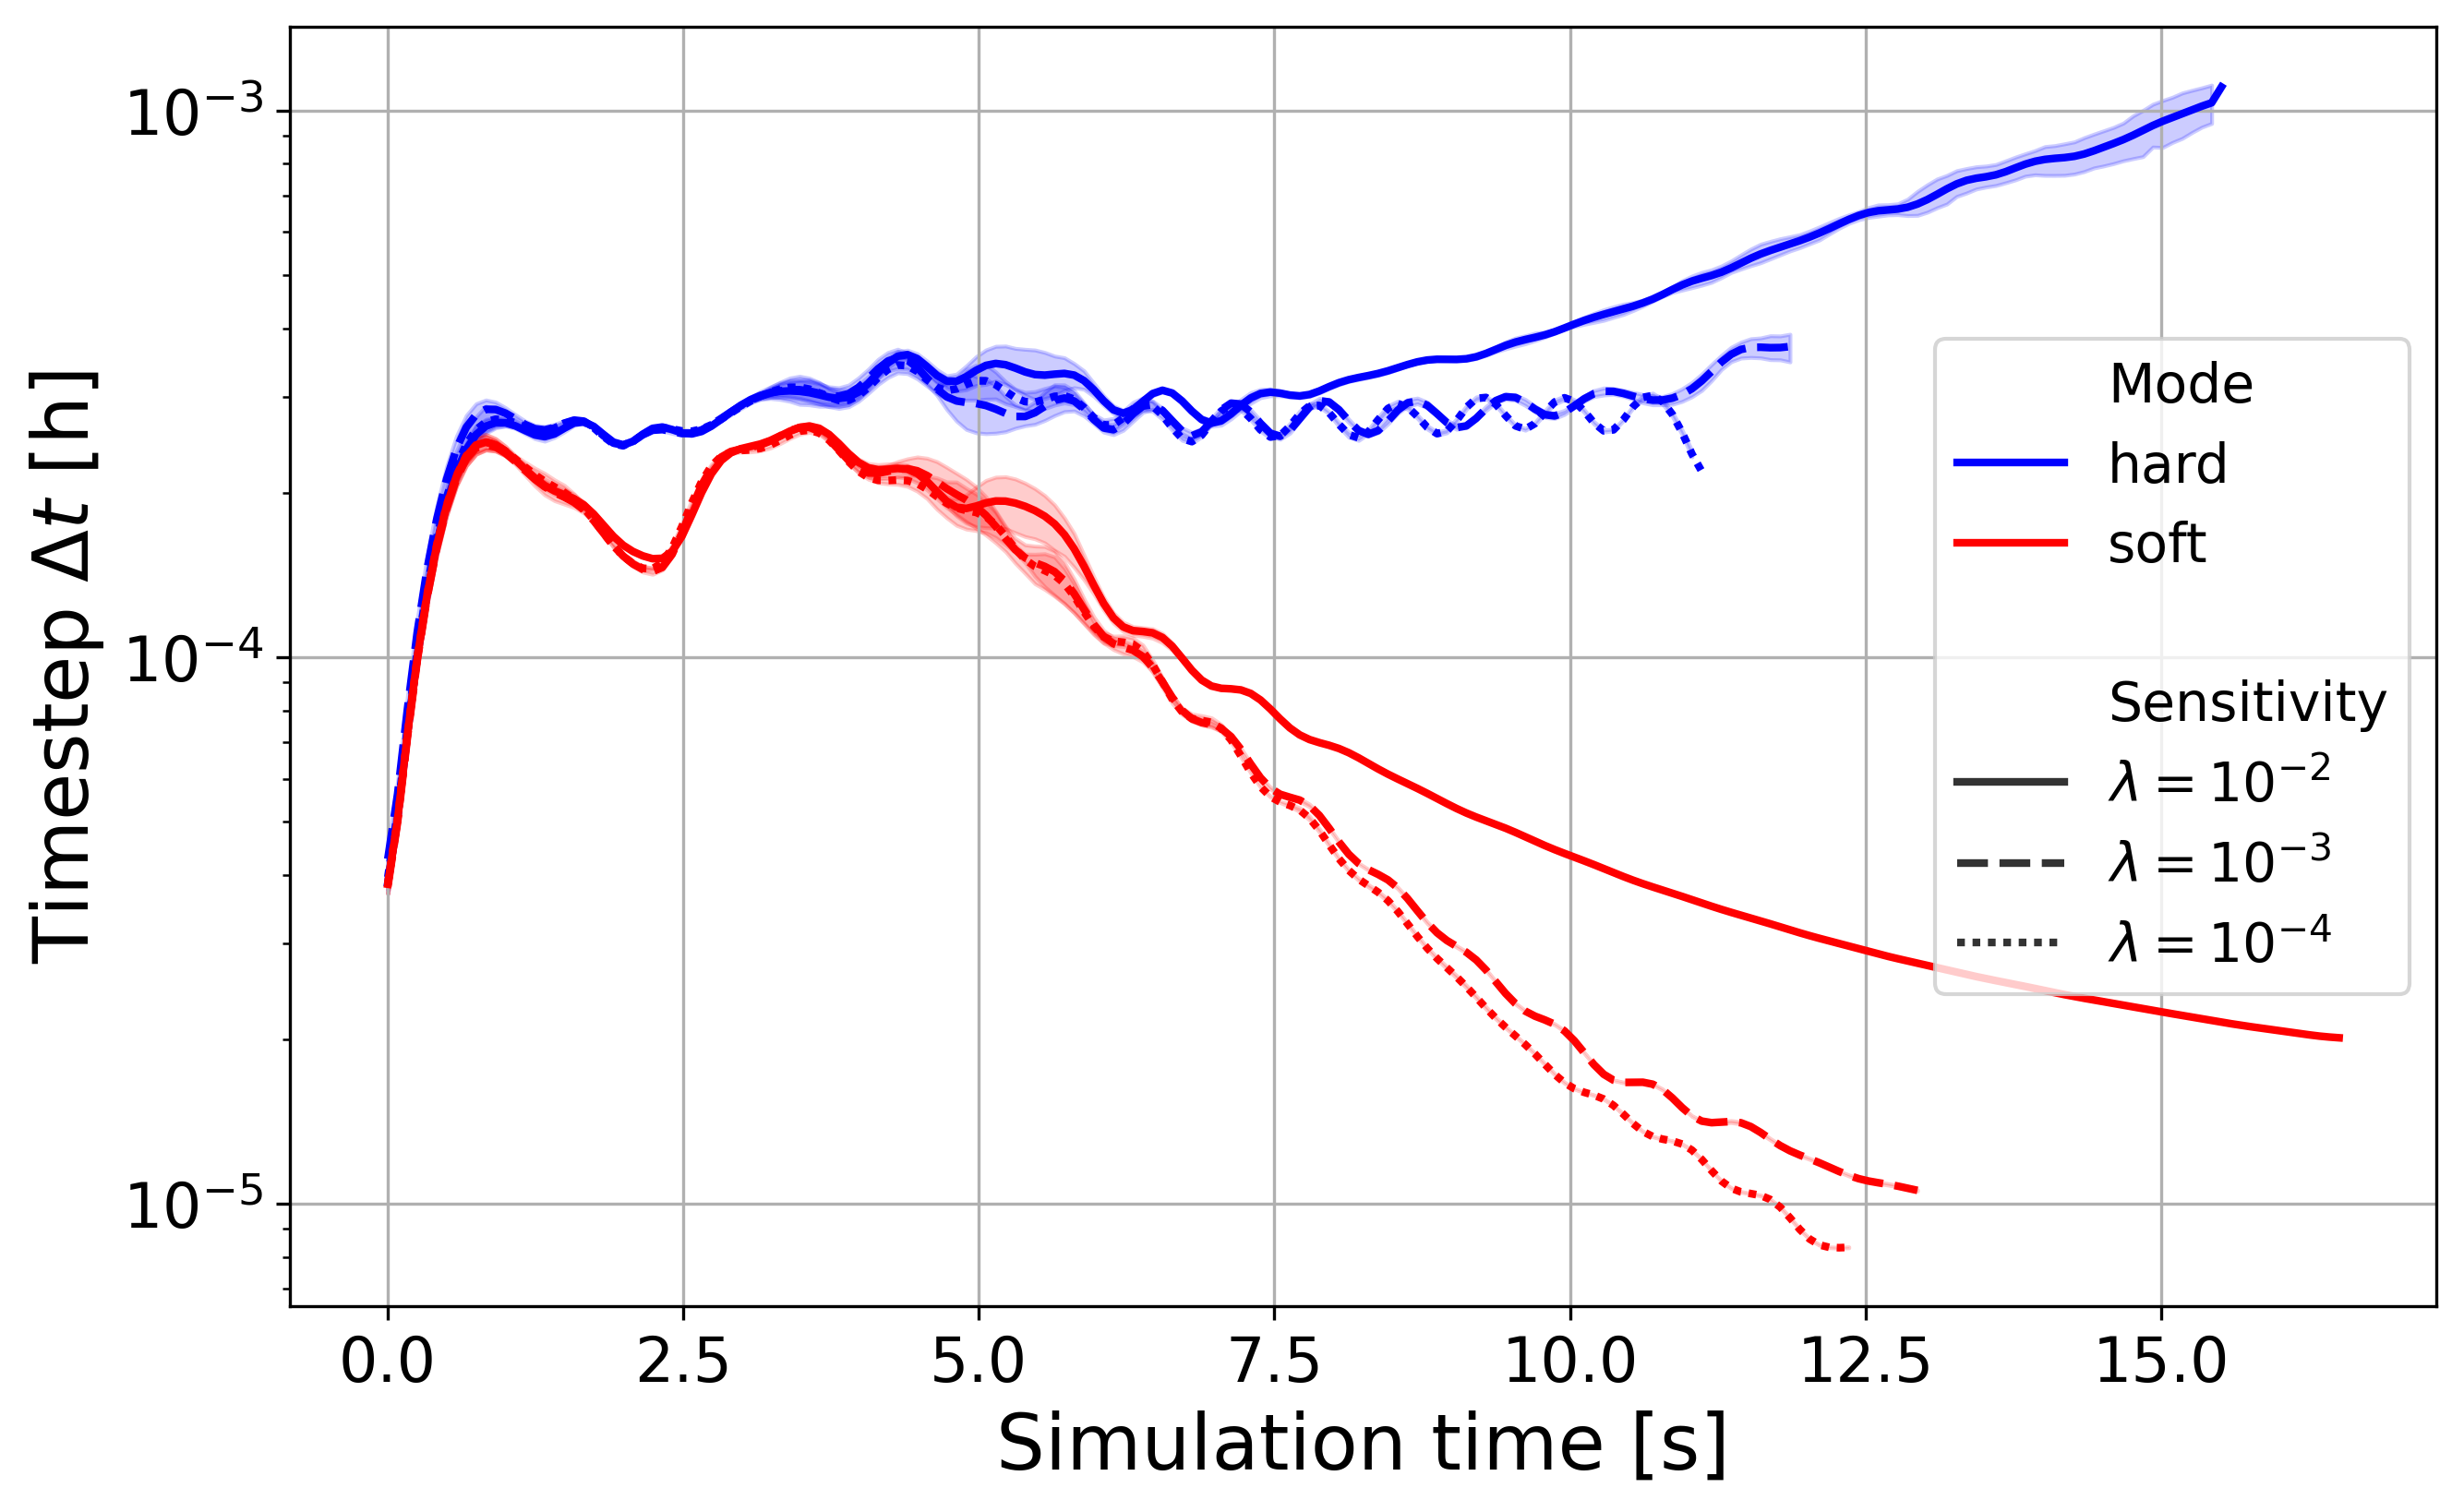
\includegraphics[width=\linewidth]{figures/comparison_plots/combined_simulation_time [s]_vs_dt.png}
    \caption{Adaptive timestep $\Delta t$ over simulation time for both collision models. The hard model stabilizes around ${\Delta t}_{\text{hard}} \approx 3 \cdot 10^{-4} h$, while the soft model decreases to ${\Delta t}_{\text{soft}} \approx 1 \cdot 10^{-5} h$.} \label{fig:simulation_time_vs_dt}
\end{figure}


\subsection{Strong Scaling}

To assess the parallel performance of the hard and soft simulation models, we analyze runtime and speedup as a function of CPU cores. Strong scaling tests start from a single particle and grow the colony to a radius of 100, revealing how efficiently each model utilizes additional cores.

At lower CPU counts ($\text{ranks}< 2^4$), the hard model is roughly 1.5x faster than the soft model (\autoref{fig:runtime_hard_soft}), likely due to its ability to take larger time steps. As core counts increase, both models converge to similar runtimes, indicating that parallelization and communication overhead dominate. Speedup analysis (\autoref{fig:speedup_hard_soft}) shows the soft model scales smoothly up to 20x for 112 ranks, while the hard model exhibits a dip at intermediate core counts, limiting its speedup to 10 before reaching a maximum of 17. This suggests that the hard model's global optimization step introduces additional communication overhead that affects scalability.

\begin{figure}[H]
    \centering
    \begin{subfigure}[b]{1\linewidth}
        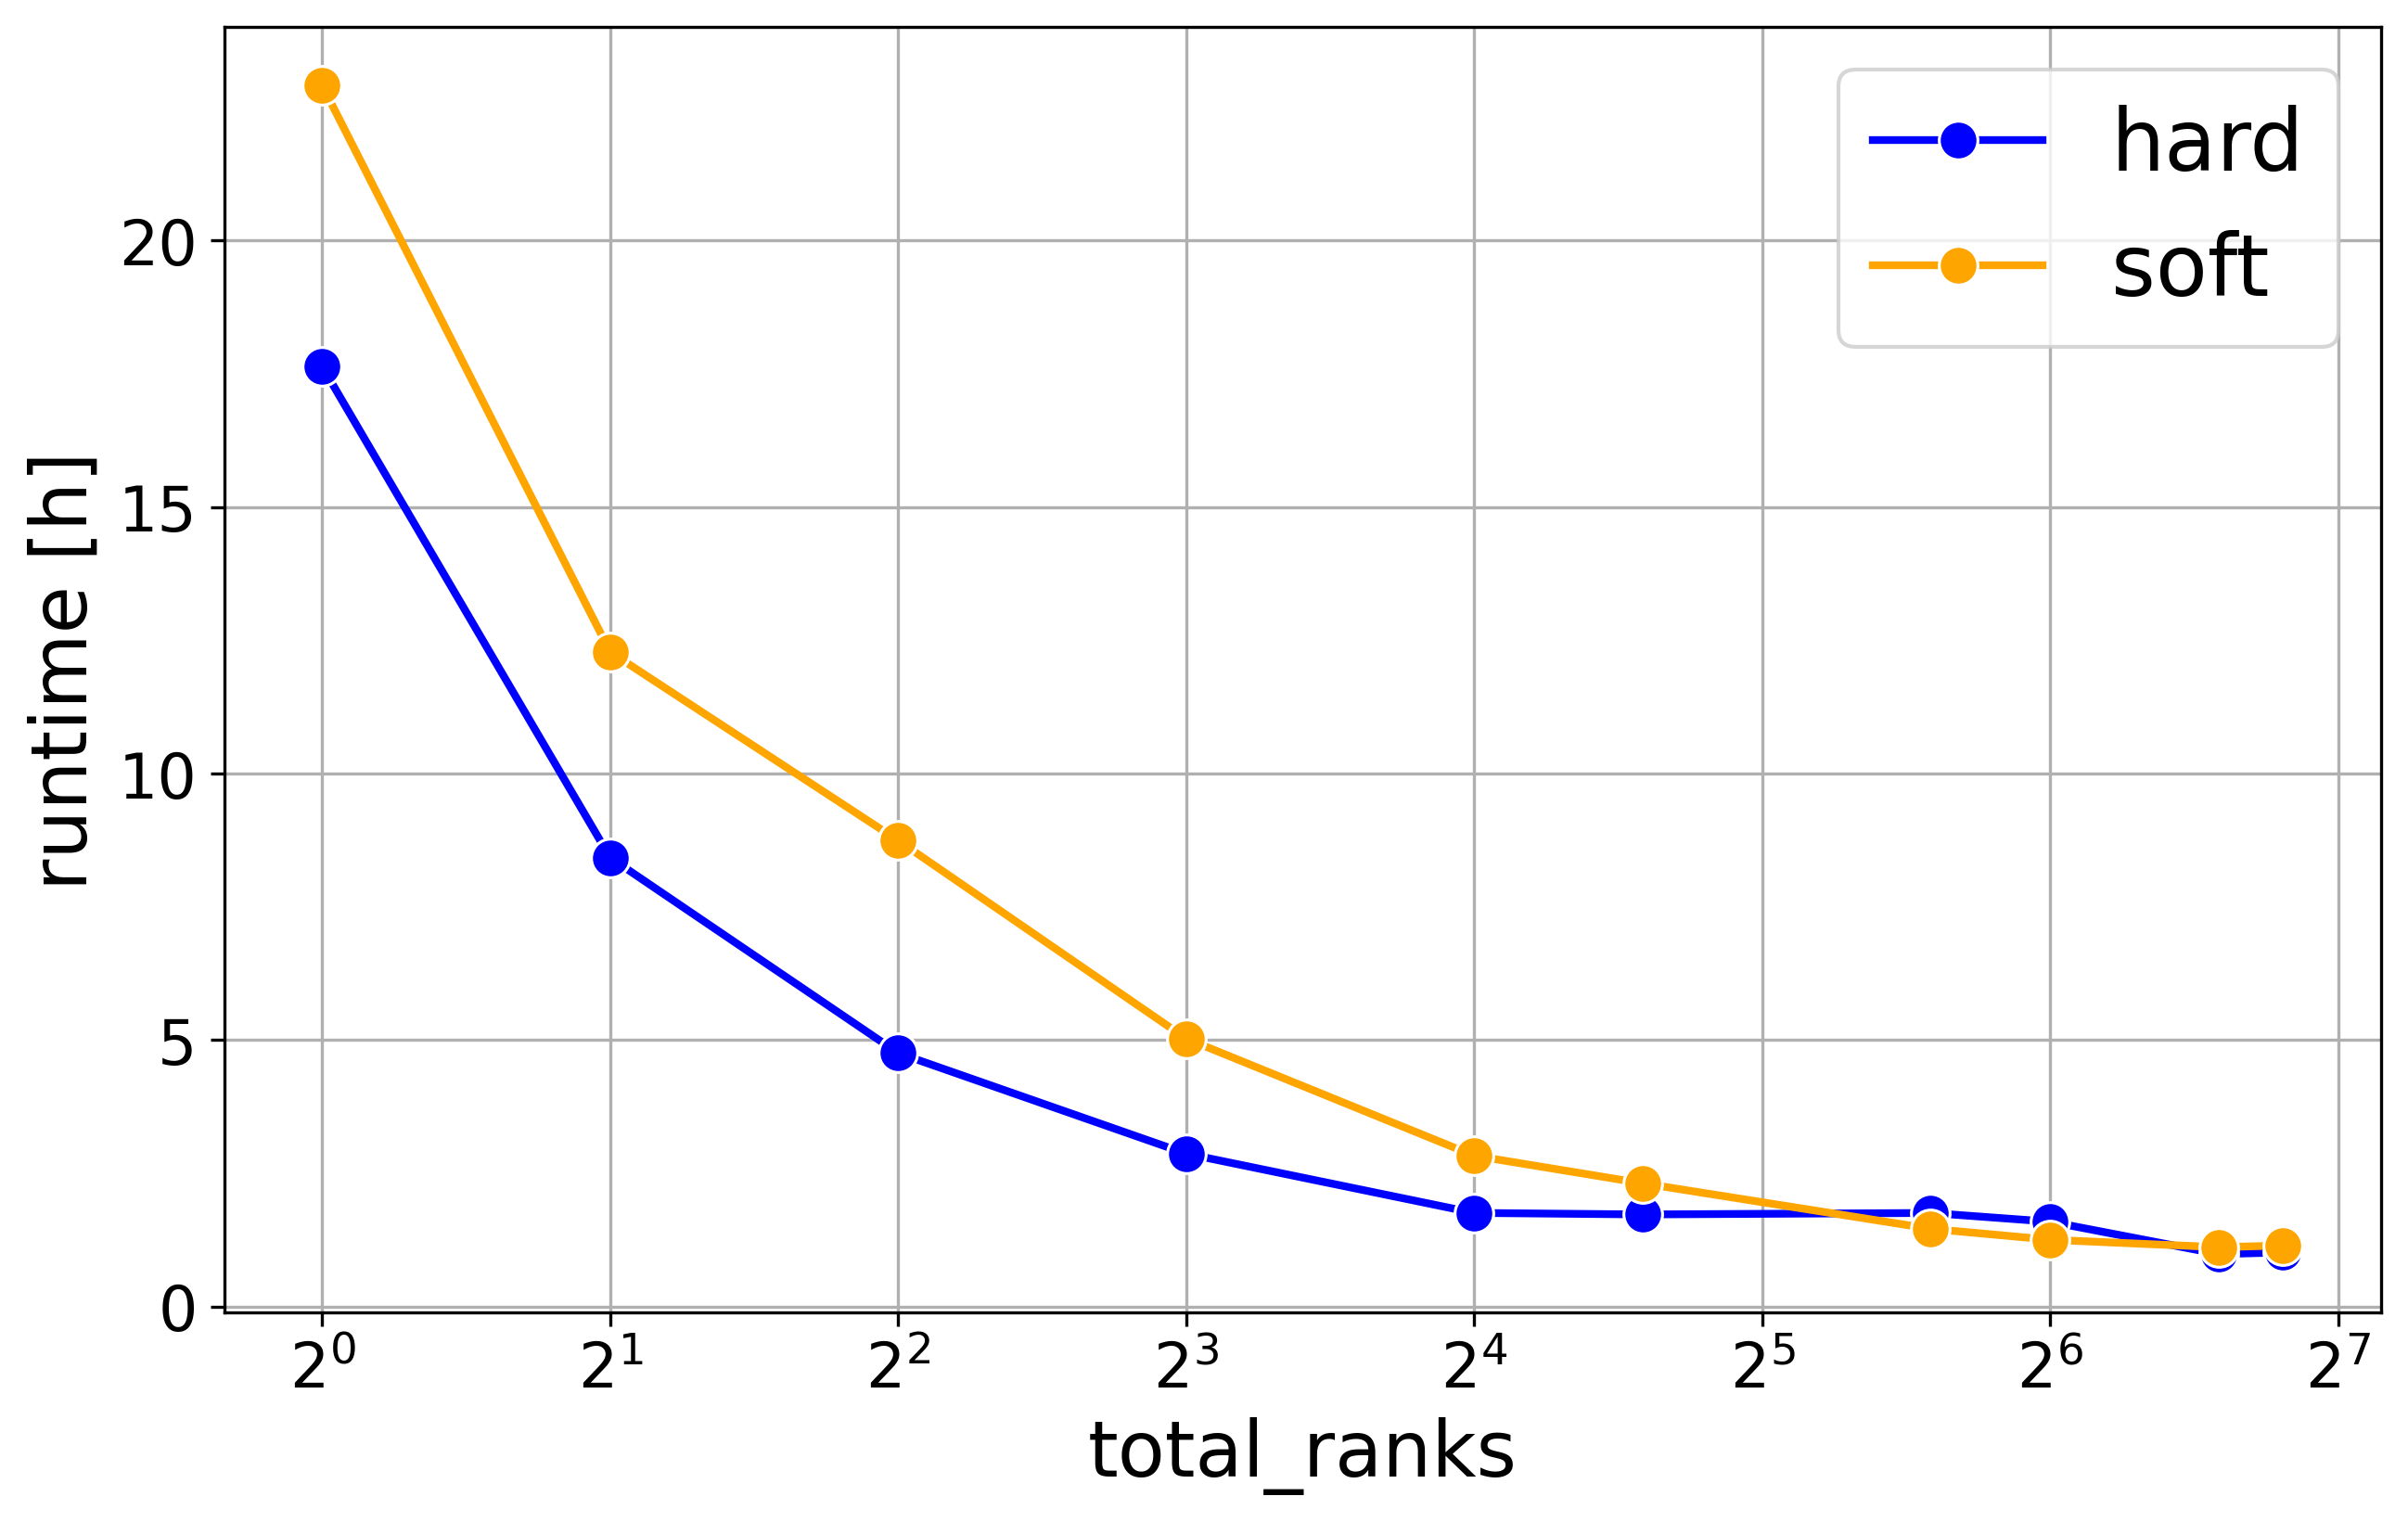
\includegraphics[width=\linewidth]{figures/runtimes/strong_scaling_hard_soft.png}
        \caption{Runtime vs CPU cores. For lower CPU counts, the hard model is about 1.5x faster than the soft model. For higher CPU counts, both models converge to similar runtimes.}
        \label{fig:runtime_hard_soft}
    \end{subfigure}

    \vspace{0.5cm}  % adds vertical space between the subfigures

    \begin{subfigure}[b]{1\linewidth}
        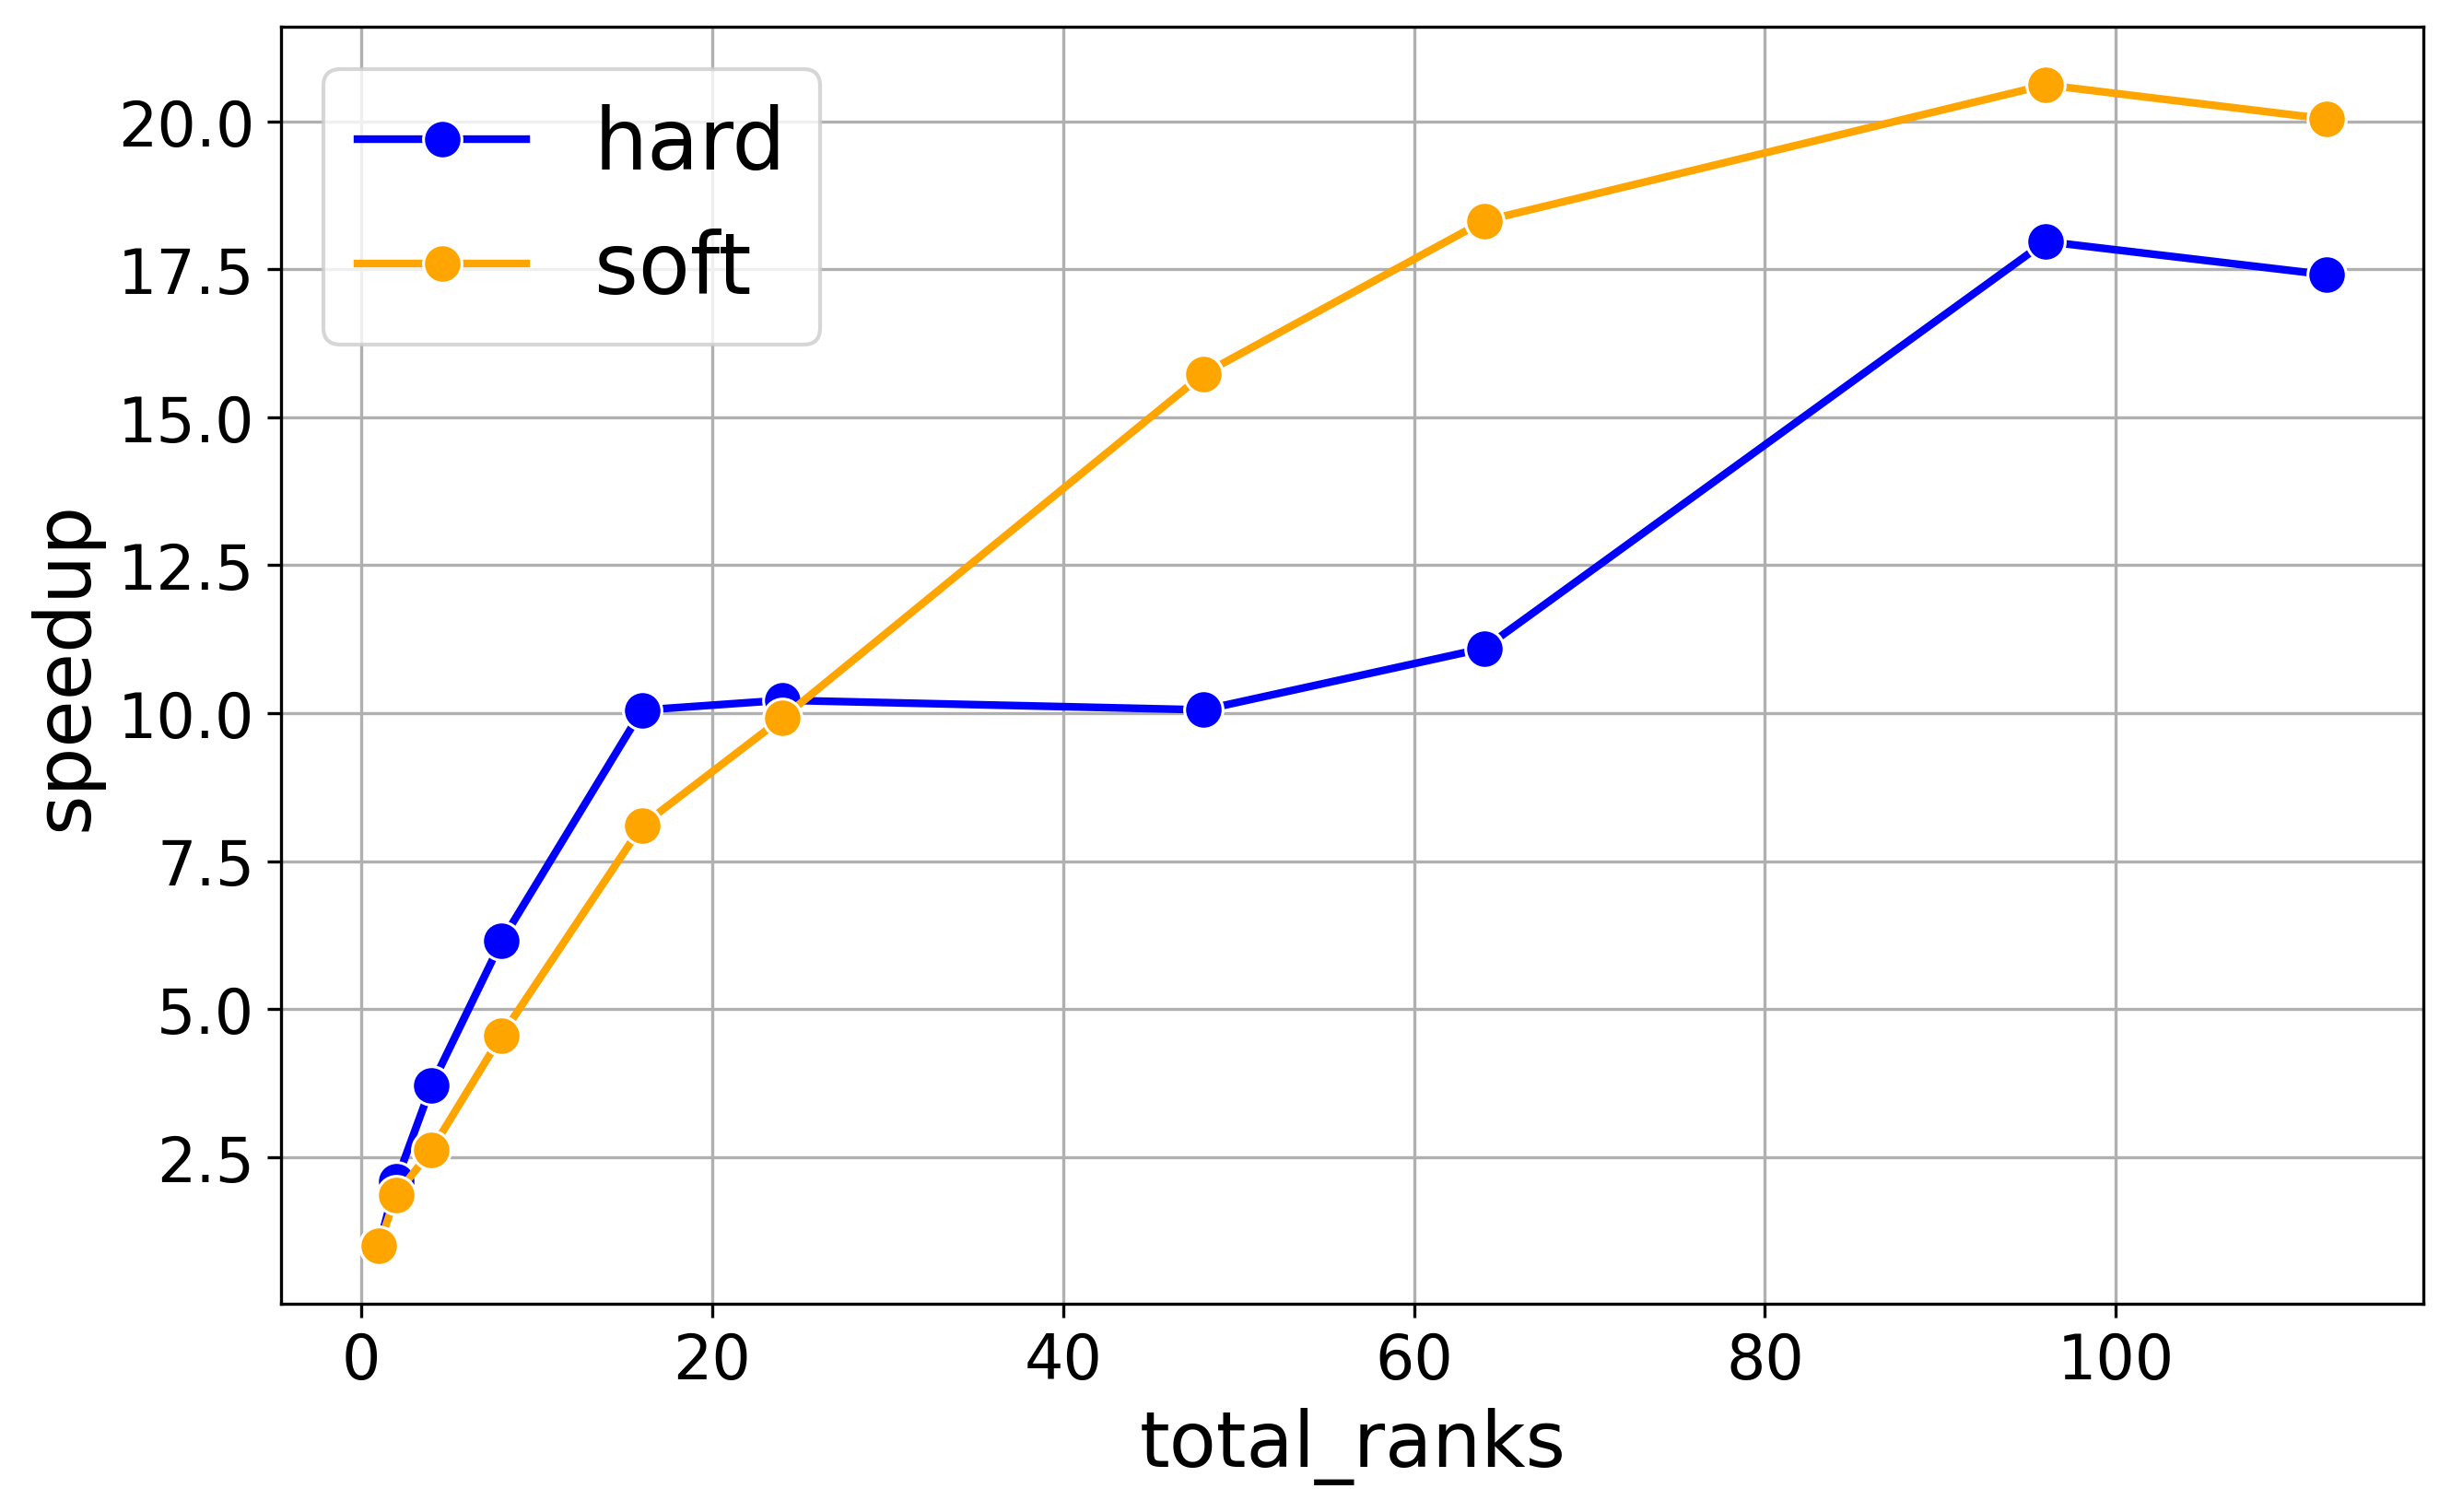
\includegraphics[width=\linewidth]{figures/runtimes/strong_scaling_efficiency_hard_soft.png}
        \caption{Speedup vs CPU cores. The soft model scales smoothly up to a speedup of 20 for 112 ranks. The hard model shows a dent in the middle, limiting speedup to 10 for intermediate CPU counts and reaching a maximum of 17.}
        \label{fig:speedup_hard_soft}
    \end{subfigure}

    \caption{Strong scaling comparison of the hard and soft models.}
\end{figure}

\subsection{Runtime and Scalability Analysis}
\label{sec:complexity_scalability}

This section delves deeper into the computational performance of both collision models by examining the walltime per particle during simulations.

As shown in \autoref{fig:walltime_per_particle}, the per-particle walltime remains approximately constant across each model but is substantially lower for the soft model. This difference arises because the soft model requires only a single force evaluation per particle, whereas the particles in the hard model contribute to global effects. \autoref{fig:walltime_per_particle} also reveals subtle temporal trends: walltime decreases slightly as particle number increases, likely due to improved load balance from domain decomposition, which allows computational cores to process particles more efficiently. Conversely, walltime increases modestly over time, presumably because each particle contributes progressively to global interactions that the solver must resolve.

A possible explanation for the hard model's increased walltime is the higher number of constraints it generates. Each ReLCP iteration introduces new constraints to resolve overlaps, leading to a denser constraint matrix. \autoref{fig:num_constraints} highlights this difference, showing that the soft model generates 6 constraints per particle (one per neighboring pair), while the hard model produces 21 constraints per particle due to the ReLCP procedure.


\begin{figure}[h]
    \centering
    \begin{subfigure}[b]{0.9\linewidth}
        \centering
        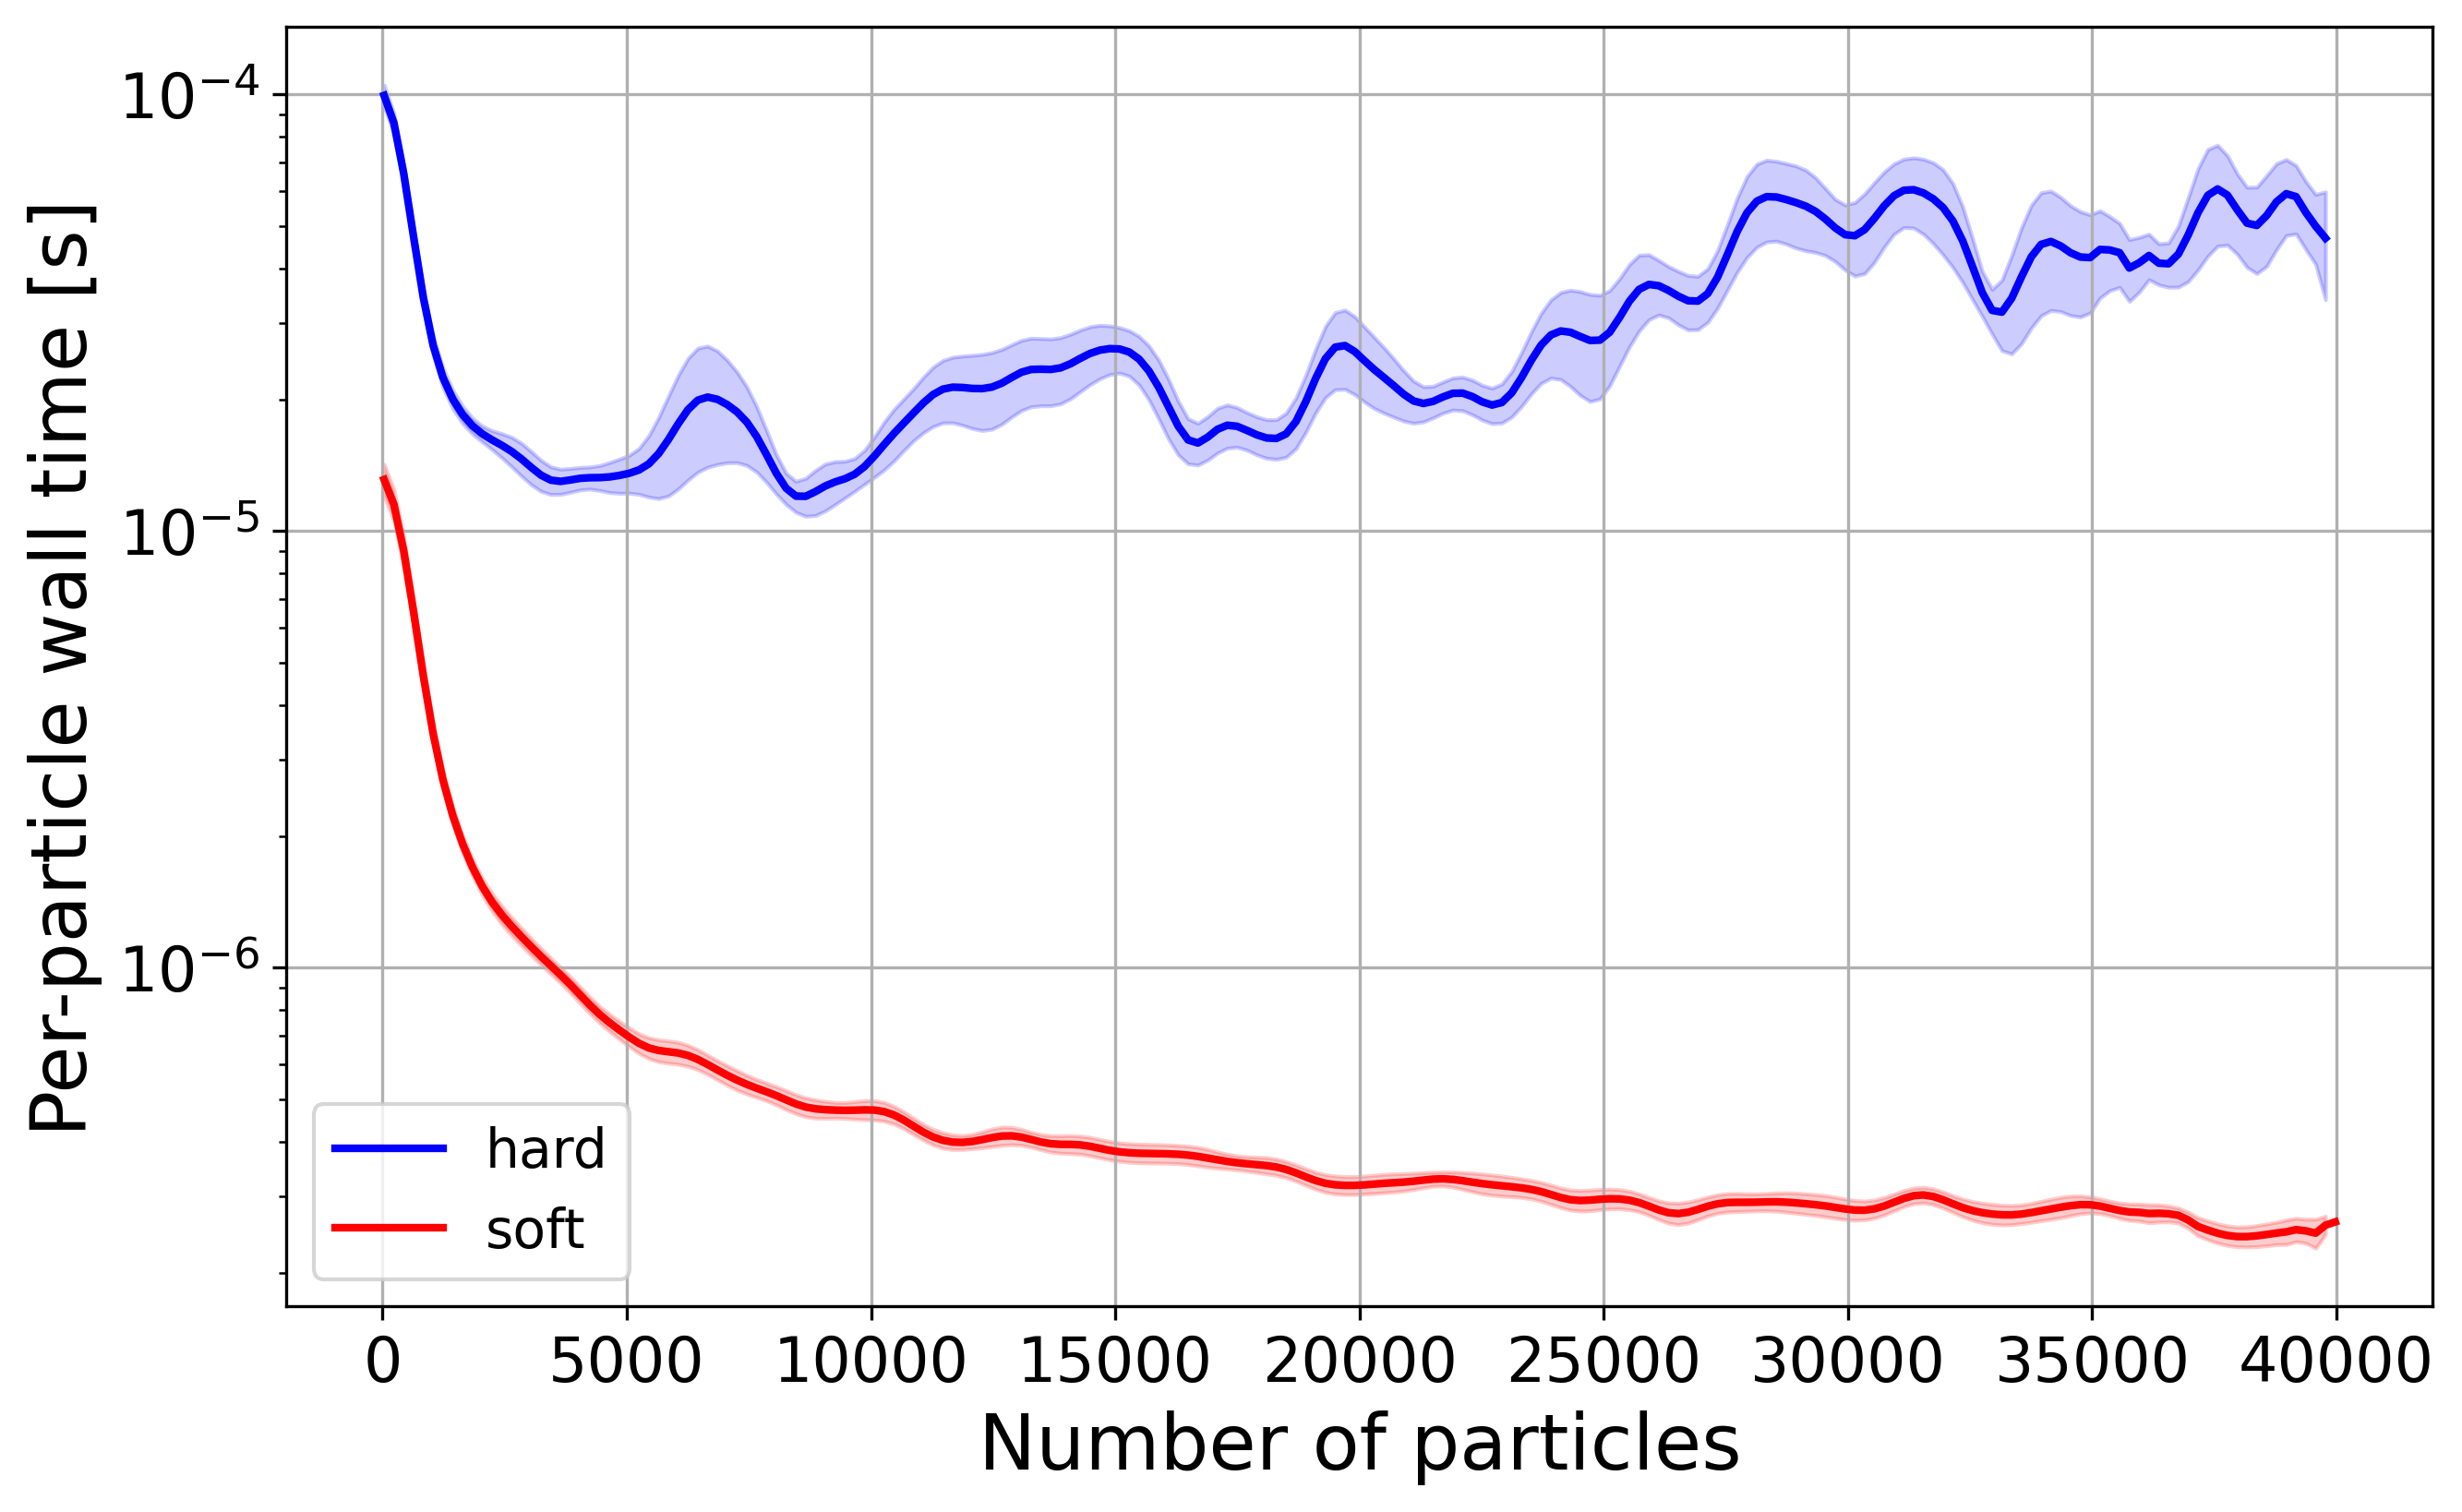
\includegraphics[width=\linewidth]{figures/comparison_plots/combined_num_particles_vs_wall_time_per_particle_with_fit.png}
        \caption{Per-particle walltime for both the hard and soft models with 112 ranks.}
        \label{fig:walltime_per_particle}
    \end{subfigure}


    \begin{subfigure}[b]{0.9\linewidth}
        \centering
        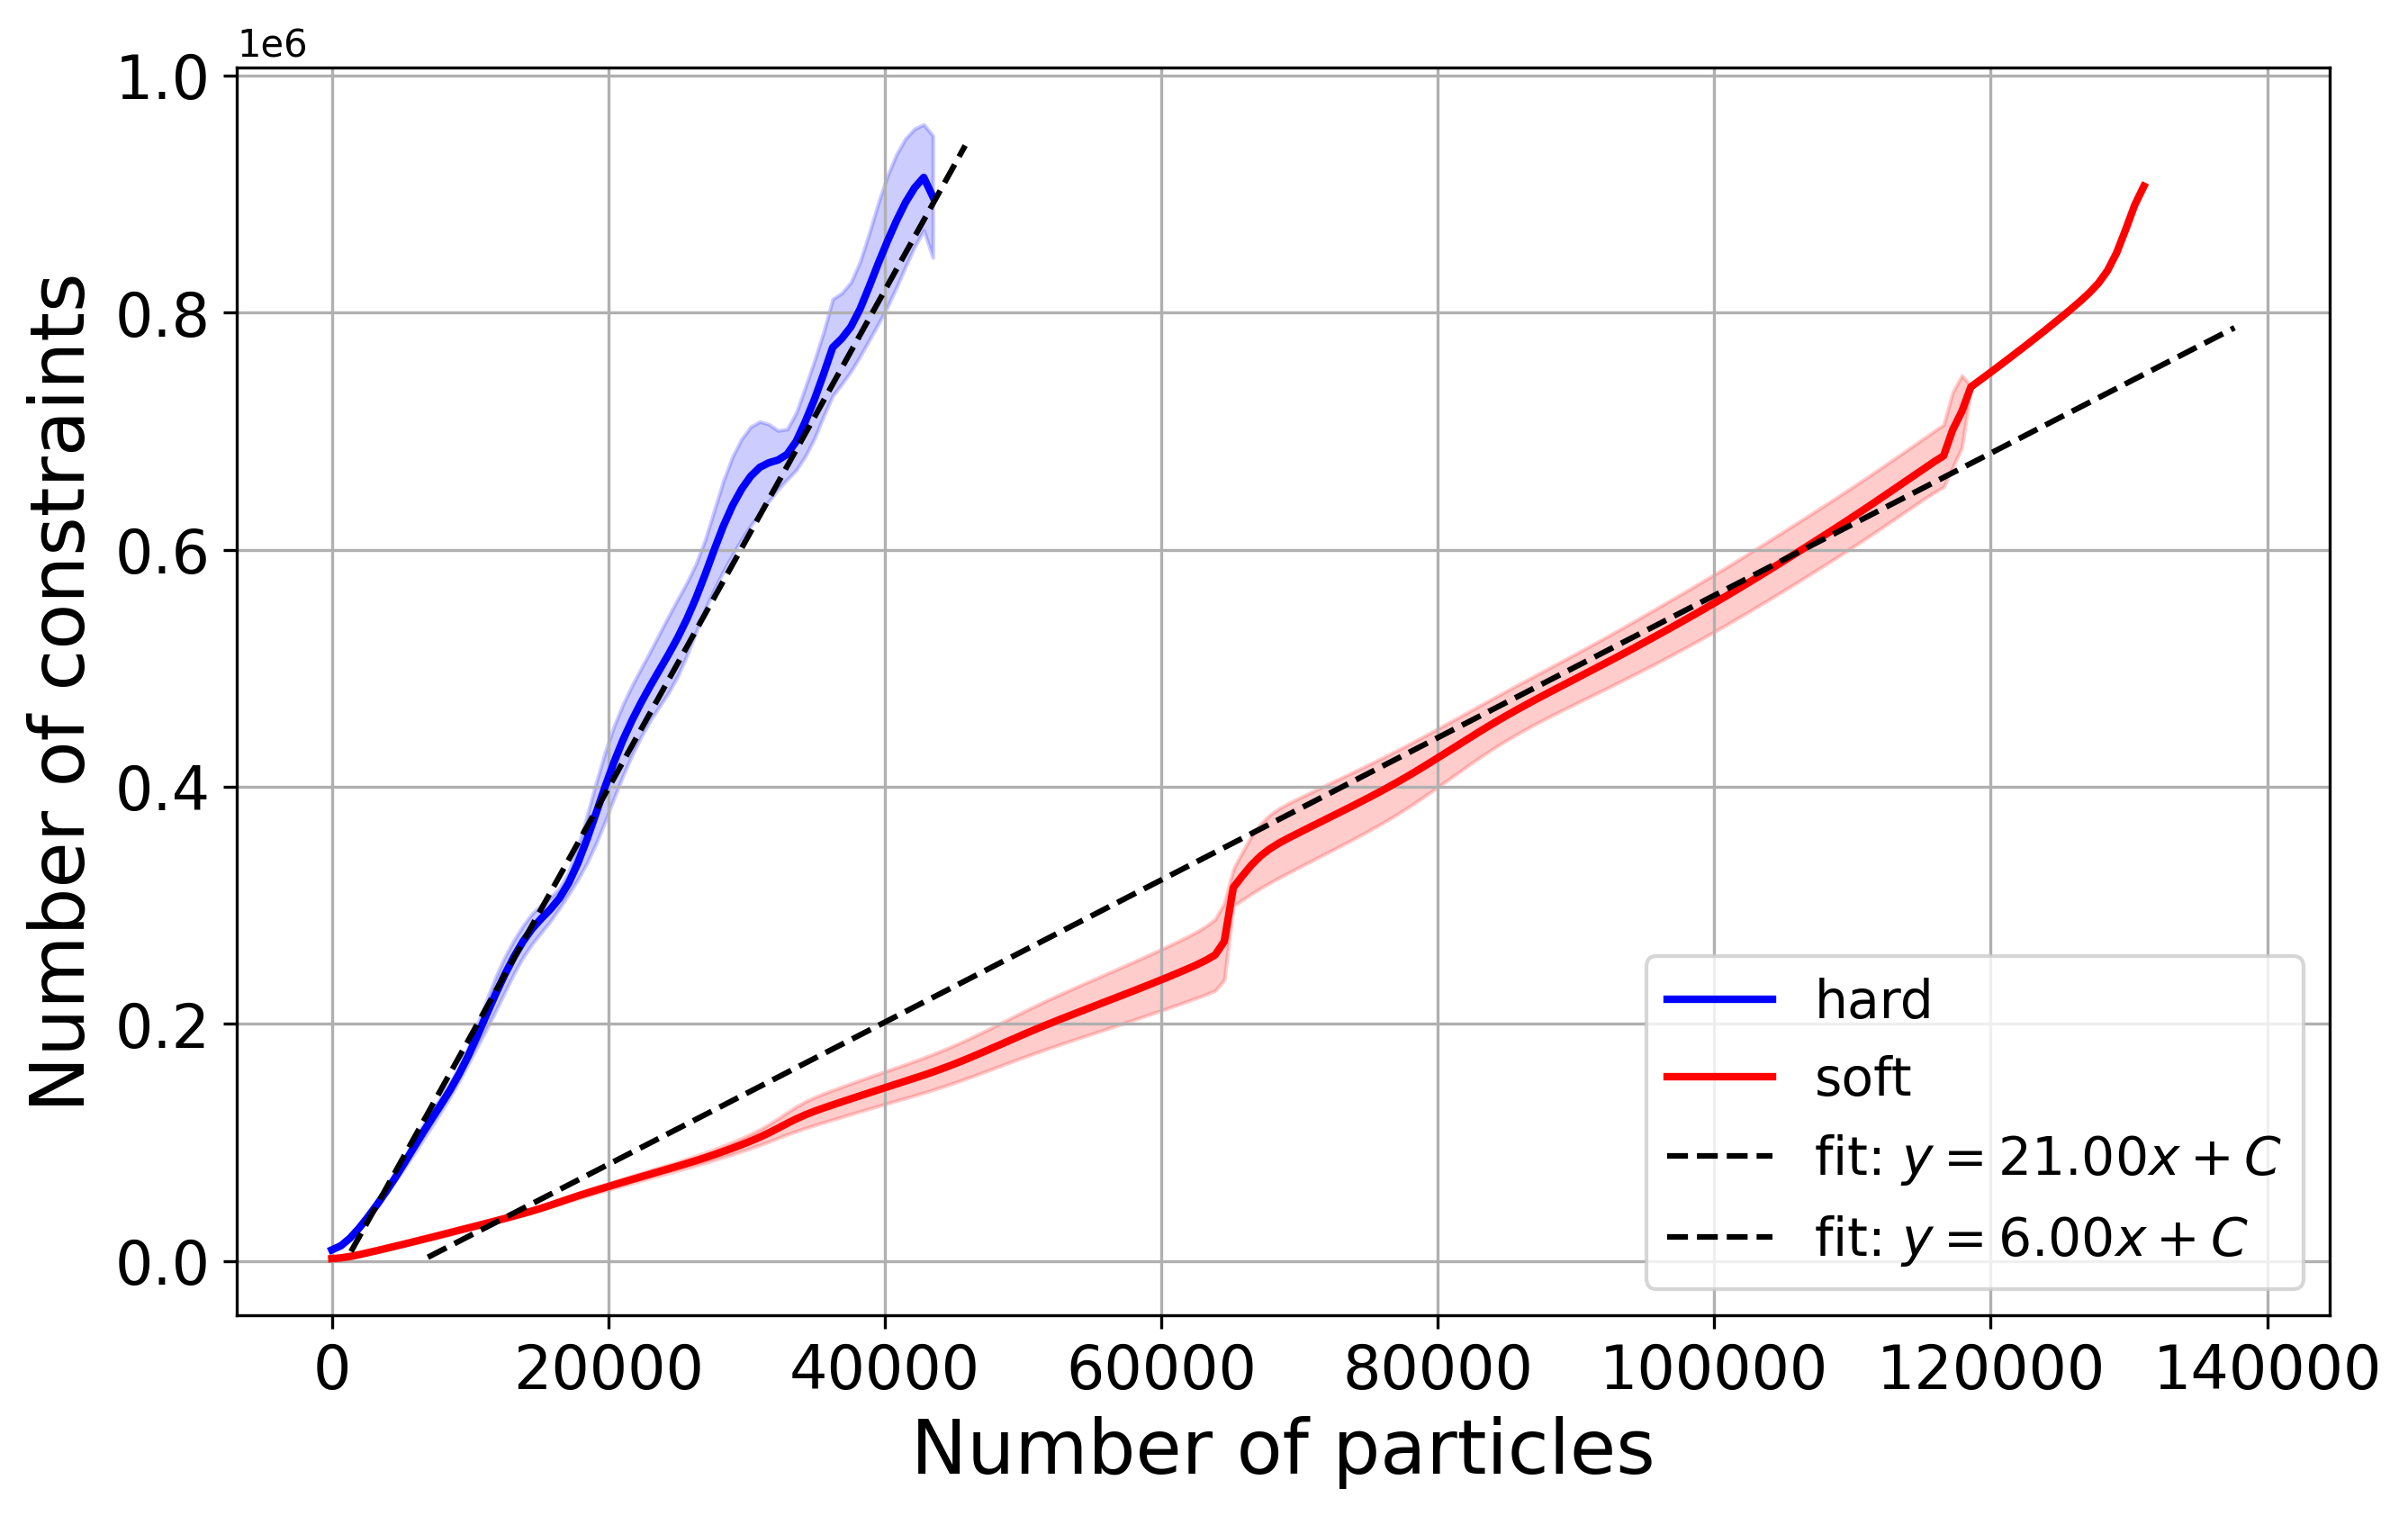
\includegraphics[width=\linewidth]{figures/comparison_plots/combined_num_constraints_vs_num_particles_with_fit.png}
        \caption{Number of constraints as a function of particle count $N$ for both models.}
        \label{fig:num_constraints}
    \end{subfigure}

    \caption{Comparison of simulation metrics for the hard and soft collision models with 112 ranks.}
    \label{fig:comparison_metrics}
\end{figure}




\newpage


\subsection{Insights into BBPGD Iterations}

The BBPGD algorithm used in the hard collision model to solve the constraint optimization problem is naturally the most costly component of the simulation. In later stages of the simulation, when the system is densely packed and many contacts need to be resolved, calls to this function, and the underlying matrix-vector operations associated with calculating the gradient, are reponsible for about 80\% of the total wall time.

It is thus crucial to understand how many BBPGD iterations are expected per time step and how this number scales with the system size. \autoref{fig:bbpgd_iterations_per_step_vs_num_particles} shows that the number of BBPGD iterations grows roughly linearly with the number of particles as $\text{bbpgd\_iterations} \approx  \frac{1}{72.3} N$.

The behavior of the BBPGD algorithm over a single time step is illustrated in \autoref{fig:bbpgd_residual}. In this iteration, the solver converges to the desired tolerance of $10^{-3}$ within about 2500 iterations, continuously decreasing the systems energy (see \autoref{eq:energy_function}) as shown in \autoref{fig:bbpgd_energy}.

For full simulations, \autoref{fig:bbpgd_iterations_histogram} shows a histogram of the number of total BBPGD iterations required per time step. This number includes extra BBPGD calls from the ReLCP procedure, which requires up to 6 iterations to fully resolve all overlaps~\cite{Weady2024SM}. The median number of iterations per time step is 470, with a long tail of more expensive steps that can require up to 30520 iterations in extreme cases. The typical number of iterations per time step is thus on the same order of magnitude as the observations in~\cite{Yan2019}, although our model is more complex due to the collision-growth coupling.



\begin{figure}[h]
    \centering
    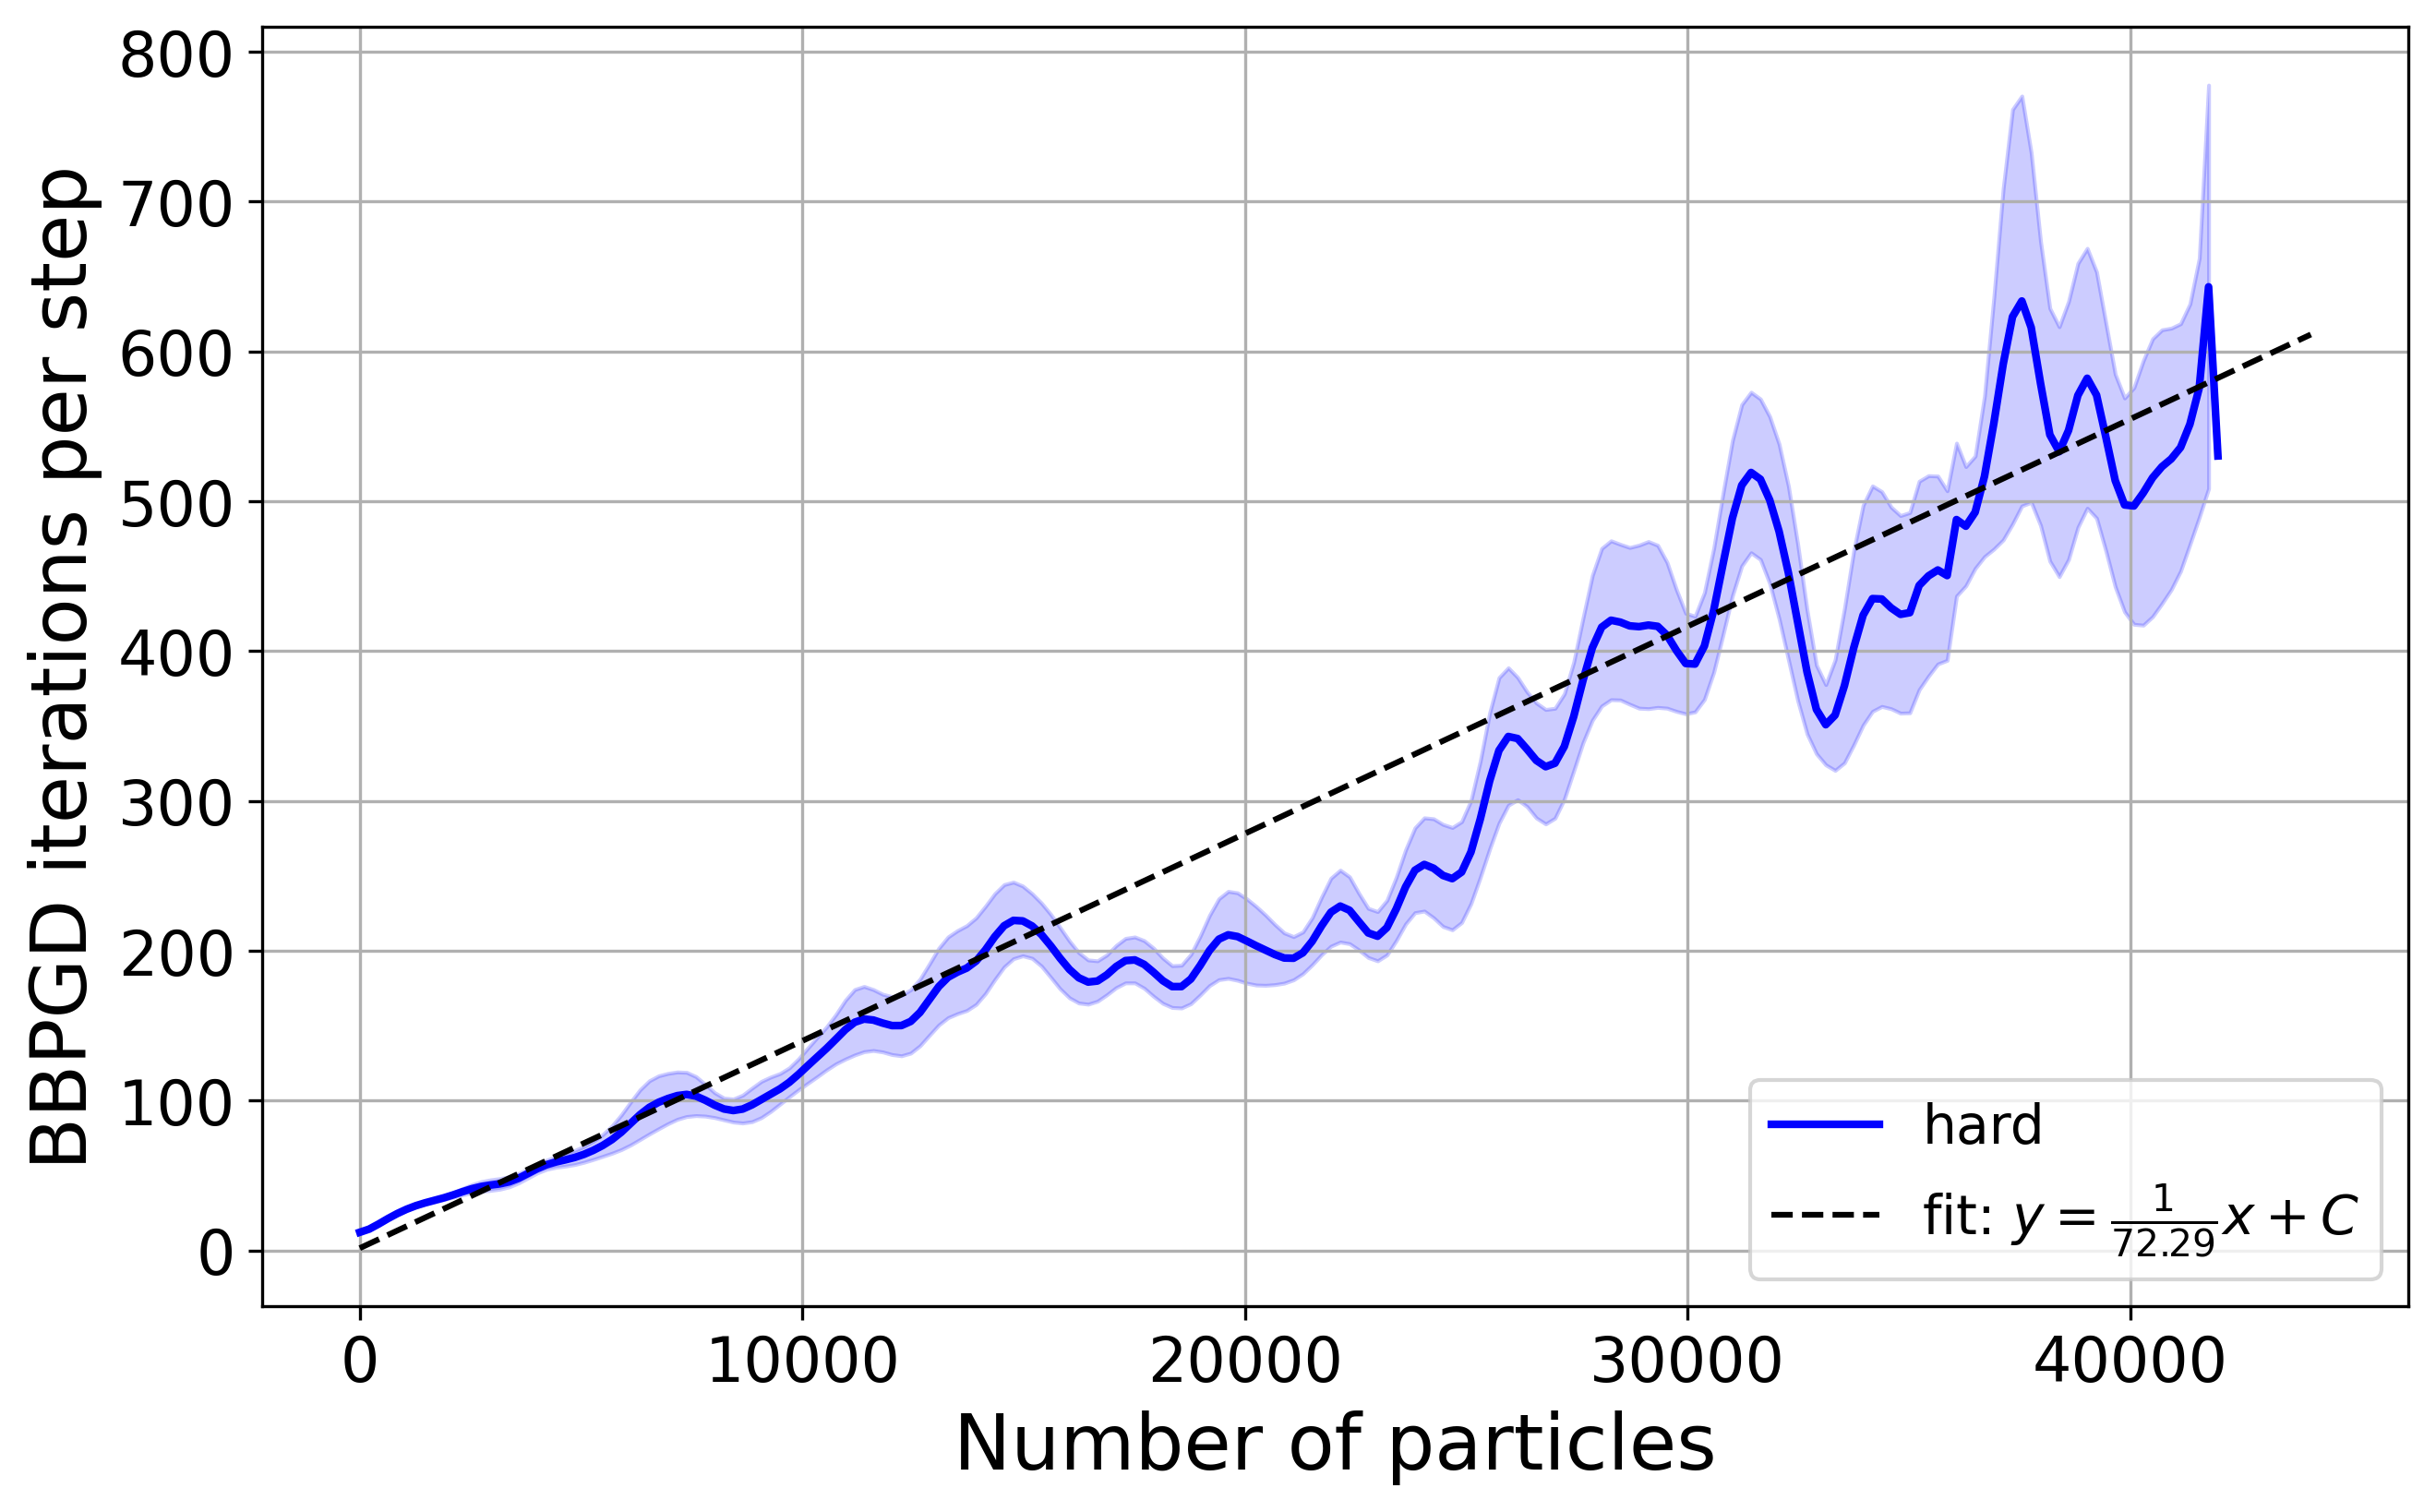
\includegraphics[width=\linewidth]{figures/comparison_plots/combined_bbpgd_iterations_per_step_vs_num_particles_with_fit.png}
    \caption{Number of BBPGD iterations per time step vs. number of particles. The number of BBPGD iterations grows roughly linearly as $\text{bbpgd\_iterations} \approx  \frac{1}{72.3} N$.}
    \label{fig:bbpgd_iterations_per_step_vs_num_particles}
\end{figure}

\begin{figure}[H]
    \centering
    \begin{subfigure}[b]{\linewidth}
        \centering
        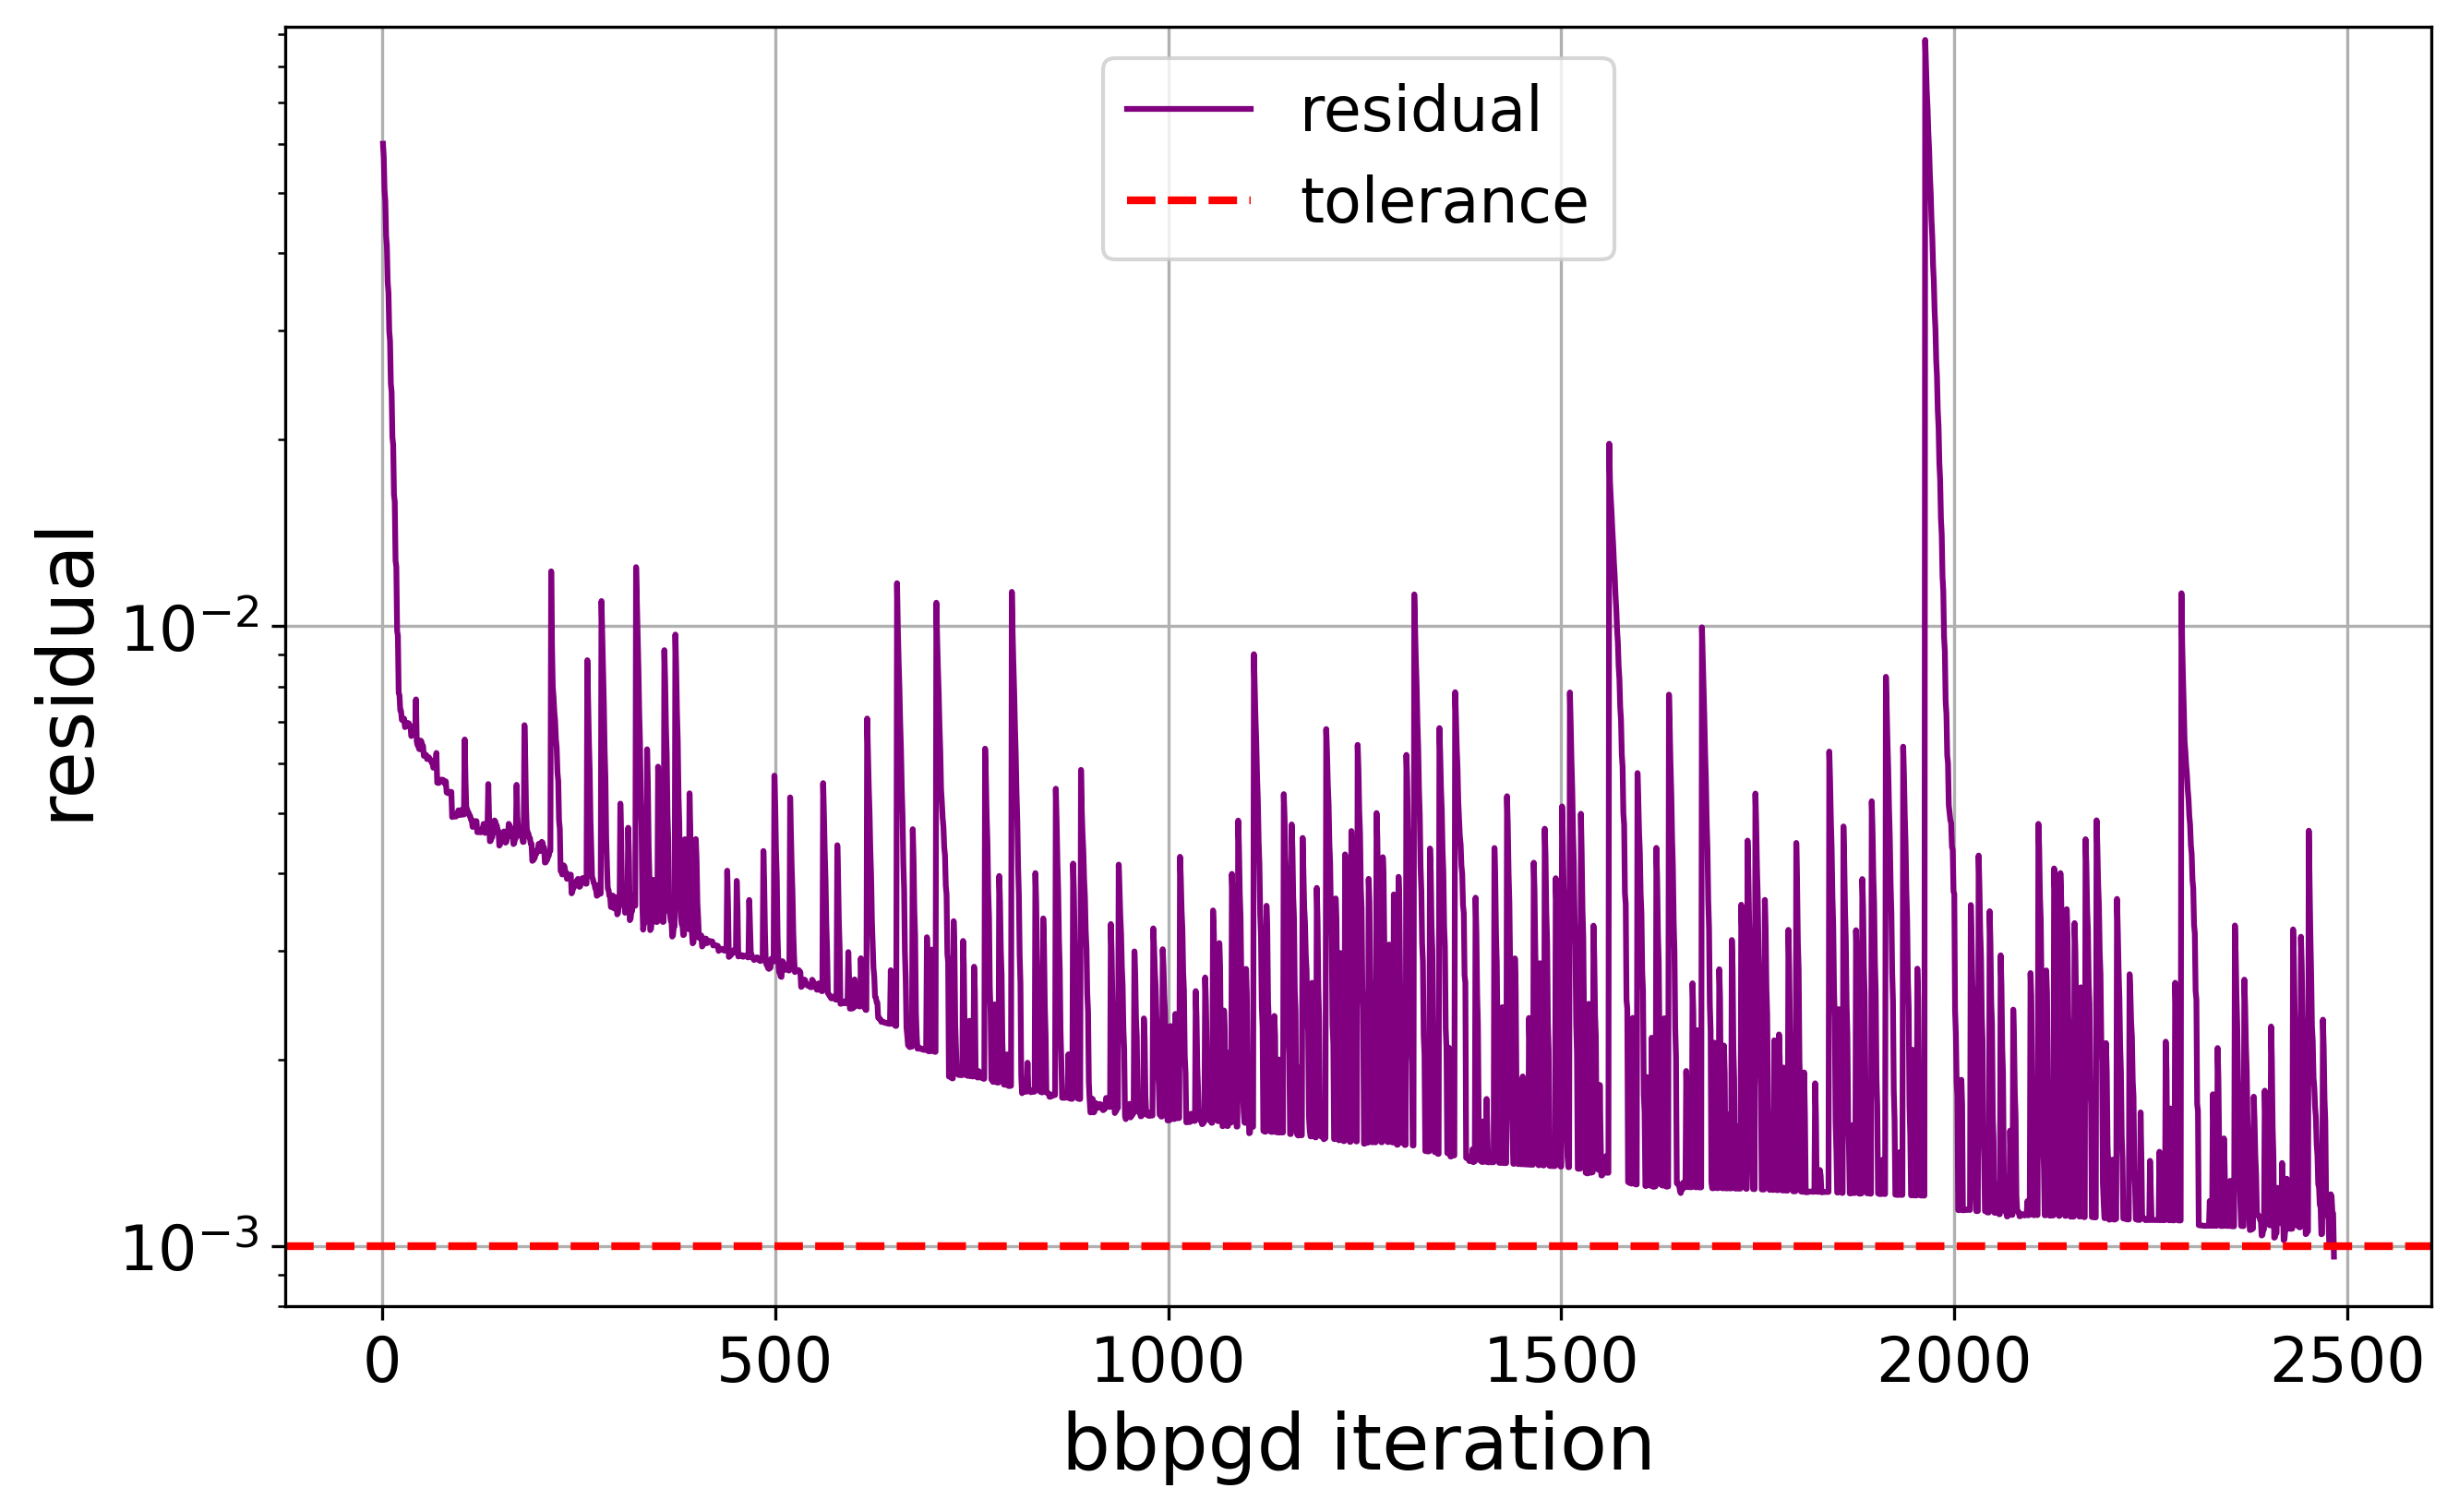
\includegraphics[width=\linewidth]{figures/comparison_plots/bbpgd_residual.png}
        \caption{BBPGD algorithm residuals over iterations for a single time step. The solver converges to the desired tolerance of $10^{-3}$ within about 2500 iterations.}
        \label{fig:bbpgd_residual}
    \end{subfigure}

    \vspace{1em}

    \begin{subfigure}[b]{\linewidth}
        \centering
        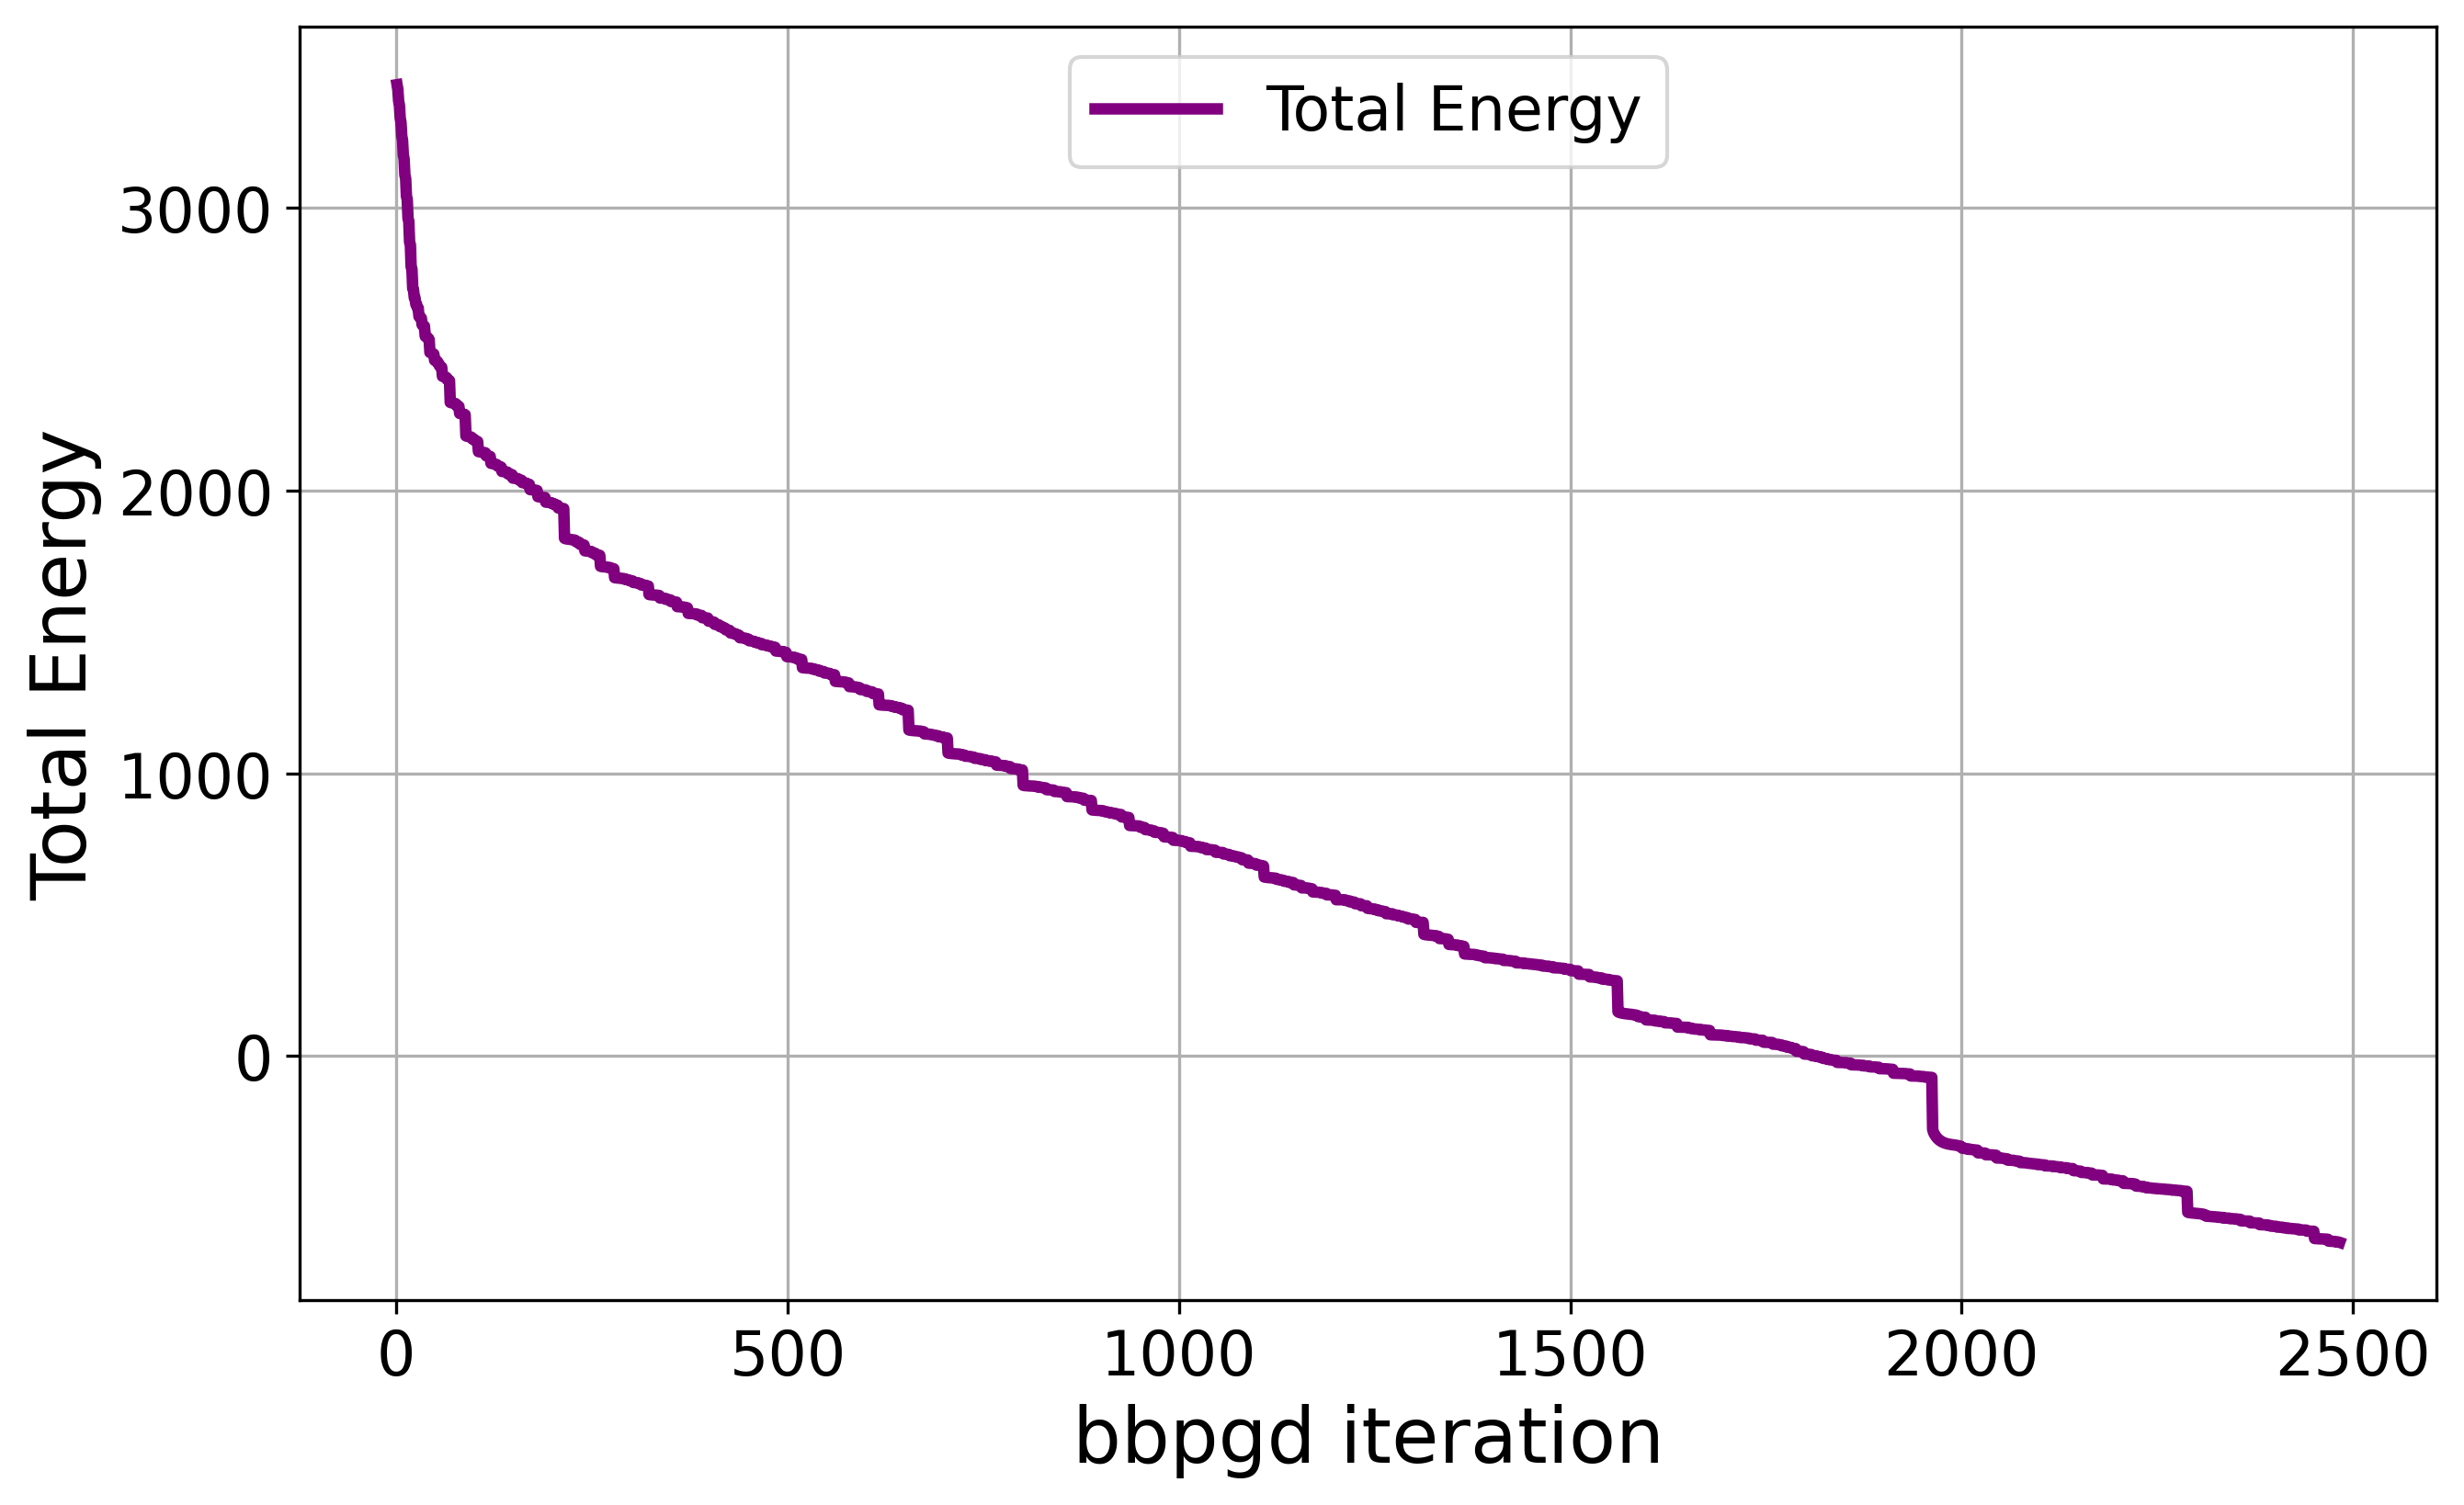
\includegraphics[width=\linewidth]{figures/comparison_plots/bbpgd_total_energy.png}
        \caption{System Energy value as described in \autoref{eq:energy_function} throughout the bbpgd algorithm. The energy decreases monotonically, confirming the convergence of the BBPGD method based on the projected gradient.}
        \label{fig:bbpgd_energy}
    \end{subfigure}

    \begin{subfigure}[b]{\linewidth}
        \centering
        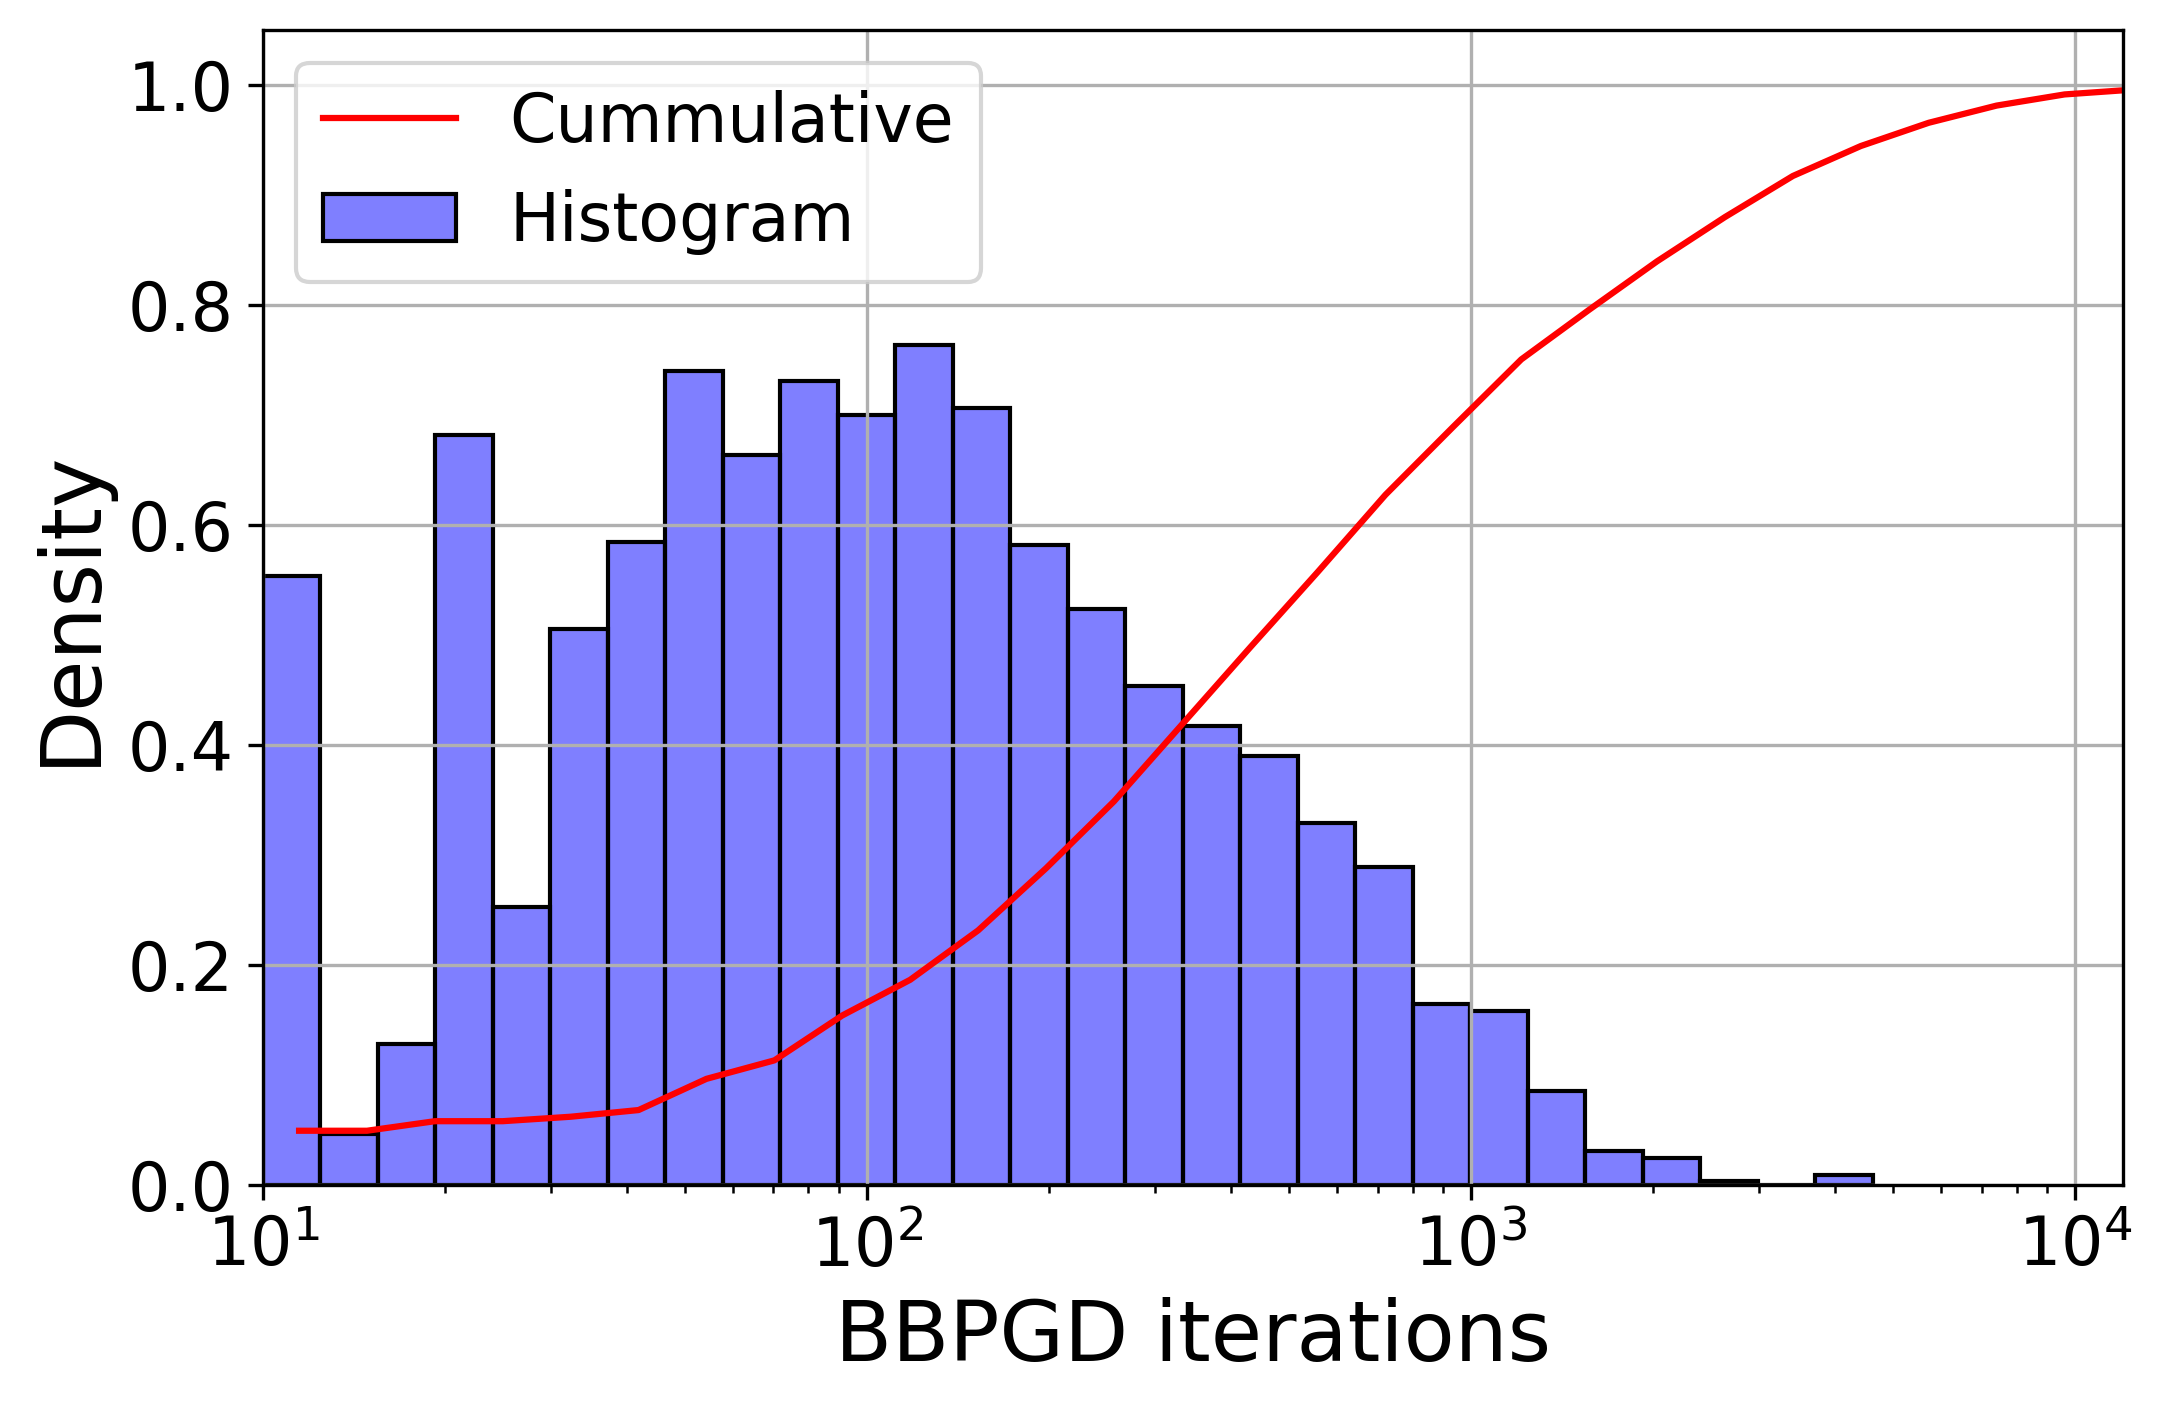
\includegraphics[width=\linewidth]{figures/comparison_plots/combined_bbpgd_iterations_histogram_cumulative.png}
        \caption{Histogram of BBPGD algorithm iterations per time step for simulations up to a colony radius of 100. The median number of iterations per time step is 470.}
        \label{fig:bbpgd_iterations_histogram}
    \end{subfigure}

    \caption{BBPGD algorithm behavior during a single time step and across a full simulation.}
\end{figure}

\clearpage
\newpage







\newpage
\clearpage

\section{Discussion}

\subsection{Model Selection Insights}

The choice between hard and soft collision models involves a clear trade-off between physical fidelity and computational efficiency.
The hard model enforces strict non-overlap, which can be useful for capturing precise mechanical interactions or stress distributions in densely packed cell populations. However, it comes at considerable computational cost, requiring iterative global solvers and limiting scalability to large systems or long simulations.

By contrast, the soft model uses continuous repulsive potentials to approximate collisions. This approach is computationally efficient and scalable, making it well-suited for exploring large colonies or wide parameter spaces.

Importantly, for many emergent pattern-formation scenarios—such as concentric ring formation—the exact enforcement of non-overlap seems less critical. Other factors, such as stress-dependent growth and a use of an adequate time step, appear to dominate the macroscopic behavior.

In this context, the soft model provides a realistic approximation of cellular interactions: biological cells are deformable, and mechanical interactions in vivo are rarely perfectly rigid. Indeed, recent studies~\cite{Khan_2024, Ghosh2015, SantosDiaz2025} suggest that finite stiffness or soft repulsive forces are sufficient to capture key structural and morphological features of growing bacterial colonies.

\subsection{Biological Relevance}

Our results indicate that the soft collision model successfully reproduces major emergent patterns despite its simplified mechanics. This aligns with the view that colony-level behaviors are robust to the details of individual cell interactions, provided that key features like stress-dependent growth are captured.

Furthermore, the soft model naturally represents continuous pressure and proximity effects, which are biologically more plausible than instantaneous, perfectly rigid constraints. This makes it a compelling choice for simulating biological systems where cells exhibit elasticity and deformability.

\section{Conclusion}

This paper demonstrates that a computationally efficient soft collision model can reproduce complex emergent patterns in proliferating cell collectives, including concentric rings observed in bacterial colonies.

While hard collision models offer exact non-overlap and may be valuable when studying precise mechanical stresses or jamming phenomena, they are computationally intensive and less scalable. Soft models, using finite repulsion to approximate contact interactions, achieve a realistic balance between biological plausibility and computational performance.

\newpage
\section{Future Work}

The current implementation provides a functional baseline for hard collision modeling, yet significant opportunities exist for performance optimization in the constraint solver.

\subsection{Hard Collision Model}
The present PETSc-based implementation of the ReLCP constraint solver faces computational bottlenecks that limit its scalability, primarily due to dynamic memory management strategies for constraint matrices and vectors. While an allocation factor mitigates frequent reallocations, sudden increases in collision events still trigger costly memory recopies. Furthermore, allocated memory is not reused between solver iterations, necessitating complete cleanup and reallocation at each time step.

Future work should focus on developing a more sophisticated memory management strategy that leverages PETSc's advanced features, such as memory pooling for constraint matrices and vectors, matrix preallocation routines with accurate nonzero pattern prediction, and incremental growth strategies to minimize MPI synchronization overhead.


\subsection{GPU Acceleration}

\cite{Tasora2008}

\subsection{Soft Collision Model}

Beyond optimizing the hard model's solver, a promising avenue is the acceleration of the soft model using advanced molecular dynamics techniques. Libraries like AutoPas~\cite{AutoPasGithub,Gratl2019,Newcome2023} offer a node-level auto-tuning framework specifically designed for particle simulations.AutoPas can dynamically select the optimal combination of algorithms (e.g., for particle interaction traversal and container data structures) tailored to the specific simulation scenario and underlying hardware architecture.

Integrating such a framework could automatically accelerate the computation of repulsive forces in the soft collision model, especially for large-scale colonies where efficient neighbor-search and force evaluation are critical.

\newpage

\balance
\bibliographystyle{IEEEtran}
\bibliography{literature}
\newpage
\nobalance



\onecolumn

\appendix

\renewcommand{\thefigure}{A\arabic{figure}}
\renewcommand{\thetable}{A.\arabic{table}}
\setcounter{figure}{0}
\setcounter{table}{0}

\begin{figure}[H]
    \makebox[\textwidth][c]{
        \centering

        \begin{tabular}{r M{0.36\textwidth} M{0.36\textwidth} }
             & Hard Model & Soft Model \\
            \orientationcomparisonrow{$\lambda=10^{-2}$}{-2}
            \orientationcomparisonrow{$\lambda=10^{-3}$}{-3}
            \orientationcomparisonrow{$\lambda=10^{-4}$}{-4}
        \end{tabular}
    }

    \caption{Comparison of orientation patterns at different stress sensitivities in the center of the colony. The color indicates the cells orientation, with similar colors representing similar angles. The hard model is able to maintain visible patches of aligned cells for all stress sensitivities, whereas the soft model tends to produce long bundles of densely packed particles for low stress sensitivies. This effect is caused by a lack of seperation forces causing cells in the center of the colony to pile up.}
    \label{fig:orientation_comparison}
\end{figure}

\newpage

\begin{figure}[p]
    \centering

    % % Lambda = 10^-2 comparison

    Growth Comparison $\lambda=10^{-2}$
    \begin{tabular}{r M{0.2\textwidth} M{0.2\textwidth} M{0.2\textwidth} M{0.2\textwidth}}
        \growthcomparisonrow{hard}{e-2}{0055}{0100}{0150}{0199}
        \growthcomparisonrow{soft}{e-2}{0055}{0100}{0150}{0200}
    \end{tabular}
    % Lambda = 10^-3 comparison

    Growth Comparison $\lambda=10^{-3}$
    \begin{tabular}{r M{0.2\textwidth} M{0.2\textwidth} M{0.2\textwidth} M{0.2\textwidth}}
        \growthcomparisonrow{hard}{e-3}{0052}{0100}{0150}{0198}
        \growthcomparisonrow{soft}{e-3}{0048}{0110}{0149}{0187}
    \end{tabular}

    % Lambda = 10^-4 comparison

    Growth Comparison $\lambda=10^{-4}$
    \begin{tabular}{r M{0.2\textwidth} M{0.2\textwidth} M{0.2\textwidth} M{0.2\textwidth}}
        \growthcomparisonrow{hard}{e-4}{0051}{0100}{0140}{0192}
        \growthcomparisonrow{soft}{e-4}{0048}{0105}{0134}{0198}
    \end{tabular}

    \caption{Comparison of pattern formation between hard and soft collision models at similar colony sizes. Each row shows the colony evolutions up to a maximum colony radius of 100. The color indicates the length of the cells (short cells are darker, longer cells are lighter). Clear concentric ring pattern are visible for both models at $\lambda = 10^{-3}$ confirming the results from~\cite{Weady2024}.}
    \label{fig:pattern_formation}
\end{figure}

\clearpage
\newpage
\twocolumn
\tableofcontents

\end{document}